\documentclass[aspectratio=169, handout]{beamer}
% \documentclass[aspectratio=169]{beamer}
\usetheme{boxes}
\usecolortheme{seagull}

% slide formatting
\setlength{\parskip}{\medskipamount} 
\setlength{\itemsep}{10pt}
\setbeamersize{text margin left=15mm,text margin right=15mm} 
\setbeamertemplate{footline}[frame number]
% \setbeamertemplate{page number in head/foot}[framenumber]
% https://tex.stackexchange.com/a/333684
% Posted by samcarter, modified by community
\setbeamertemplate{footline}{
  \hfill%
  \usebeamercolor[fg]{page number in head/foot}%
  \usebeamerfont{page number in head/foot}%
  \setbeamertemplate{page number in head/foot}[framenumber]%
  \usebeamertemplate*{page number in head/foot}\kern1em\vskip6pt%
}

\usepackage[style=authoryear]{biblatex}
\addbibresource{refs.bib}
\AtBeginBibliography{\footnotesize}
\usepackage[colorlinks=true, citecolor=gray]{hyperref}
% Color all text, parentheses, and notes in citations gray
\usepackage{xcolor}
\AtEveryCite{\color{gray}}
\AtEveryMultiCite{\color{gray}}

\usepackage{soul}
\definecolor{Light}{gray}{.90}
\sethlcolor{Light}

% Title %%%%%%%%%%%%%%%%%%%%%%%%%%%%%%%%%%%%%%%%%%%%%%%%%%%%%
\title{(ADA) Texture representation in the visual processing hierarchy}
\author{Al Xin, axin@andrew.cmu.edu}
\institute{Statistics Advisor: Rob Kass. External Advisor: Jenelle Feather (Psych and NI)}
\date{November 23, 2026} 

\usefonttheme[onlymath]{serif}
% Symbols %%%%%%%%%%%%%%%%%%%%%%%%%%%%%%%%%%%%%%%%%%%%%%%%%%%%%

\usepackage{amsthm}
\usepackage{amsmath}
\usepackage{amssymb}
\usepackage{amsfonts}

% New commands %%%%%%%%%%%%%%%%%%%%%%%%%%%%%%%%%%%%%%%%%%%%%%%%

% General mathematical symbols
% argmin help from egreg from tex.stackexchange.com/questions/5223
\newcommand{\R}{\mathbb{R}}
\newcommand{\onedim}{\mathbb{R}}
\newcommand{\ddim}{\mathbb{R}^d}
\newcommand{\kdim}{\mathbb{R}^k}

\newcommand{\eps}{\varepsilon}
\newcommand{\seq}[1]{\{ #1_{n} \}}
\newcommand{\bfs}[1]{\boldsymbol{ #1 }}

\DeclareMathOperator*{\sign}{sign}
\DeclareMathOperator*{\argmin}{arg\,min}
\DeclareMathOperator*{\argmax}{arg\,max}
\DeclareMathOperator*{\dist}{dist}
\DeclareMathOperator*{\diag}{diag}

% boldface
\newcommand{\bfX}{\mathbf{X}}
\newcommand{\bfx}{\mathbf{x}}
\newcommand{\bfY}{\mathbf{Y}}
\newcommand{\bfy}{\mathbf{y}}
\newcommand{\bfZ}{\mathbf{Z}}
\newcommand{\bfz}{\mathbf{z}}

% Sets
\newcommand{\setA}{\mathcal{A}}
\newcommand{\setB}{\mathcal{B}}
\newcommand{\setC}{\mathcal{C}}
\newcommand{\setF}{\mathcal{F}}
\newcommand{\rademacher}{\mathcal{R}}
\newcommand{\setP}{\mathcal{P}}

% General stats
\newcommand{\E}{\mathbb{E}}
\DeclareMathOperator*{\var}{Var}
\DeclareMathOperator*{\cor}{Corr}
\DeclareMathOperator*{\cov}{Cov}
\newcommand{\prob}{\mathbb{P}}

\newcommand{\indep}{\perp \!\!\! \perp}
\newcommand{\depen}{\cancel{\indep}}
\newcommand{\indic}{\mathbbm{1}}
\newcommand{\Xbar}{\overline{X}_n}
\newcommand{\Xsqbar}{\overline{X^2_n}}
\newcommand{\Xbarsq}{\overline{X}^2_n}
\newcommand{\Ybar}{\overline{Y}_n}
\newcommand{\lik}{\mathcal{L}}
\newcommand{\ton}[1]{#1_1, \dots, #1_n}
\newcommand{\fisher}{\mathcal{I}}
\newcommand{\sumn}{\sum_{i = 1}^n}
\newcommand{\prodn}{\prod_{i = 1}^n}

% Distributions
\newcommand{\hpp}{\textrm{HPP}}
\newcommand{\ipp}{\textrm{IPP}}
\newcommand{\geom}{\textrm{Geom}}
\newcommand{\iid}{\overset{\textrm{i.i.d.}}{\sim}}
\newcommand{\pois}{\textrm{Pois}}
\newcommand{\bern}{\textrm{Bern}}
\newcommand{\N}{\mathcal{N}}
\newcommand{\MVN}{\textrm{MVN}}
\newcommand{\unif}{\textrm{Unif}}
\newcommand{\binomial}{\textrm{Binom}}
\newcommand{\expo}{\textrm{Expo}}
\newcommand{\hgeom}{\textrm{HGeom}}

\newcommand{\todo}[1]{{\color{purple}#1}}
\newenvironment{todoblock}{\color{purple}}{}

\begin{document}

\begin{frame}
\titlepage
\end{frame}

\begin{frame}{Overview}
\begin{itemize}
    % \item Successive visual processing areas are thought to be responsive to higher-level image statistics. \pause
    \item Neural responses to visual textures provide evidence for how visual areas process information. \pause
    \item Few studies of visual textures include higher-level areas due to the sparseness of responses in areas like V4 and IT. \pause 
    \item We characterize regions by the separability of visual textures \pause
    \item Differences in the \hl{reliability} and \hl{sparsity} bias these measures \pause 
    \item After correcting for reliability, IT texture separability appears comparable to V4 \pause
    \item V4 and IT show better between-family separation and worse within-family sample separation compared to V1 and V2
\end{itemize}
\end{frame}

\section{Introduction}

\begin{frame}{Regions later in the visual hierarchy select for higher level features}
  \centering
  \only<1| handout:0>{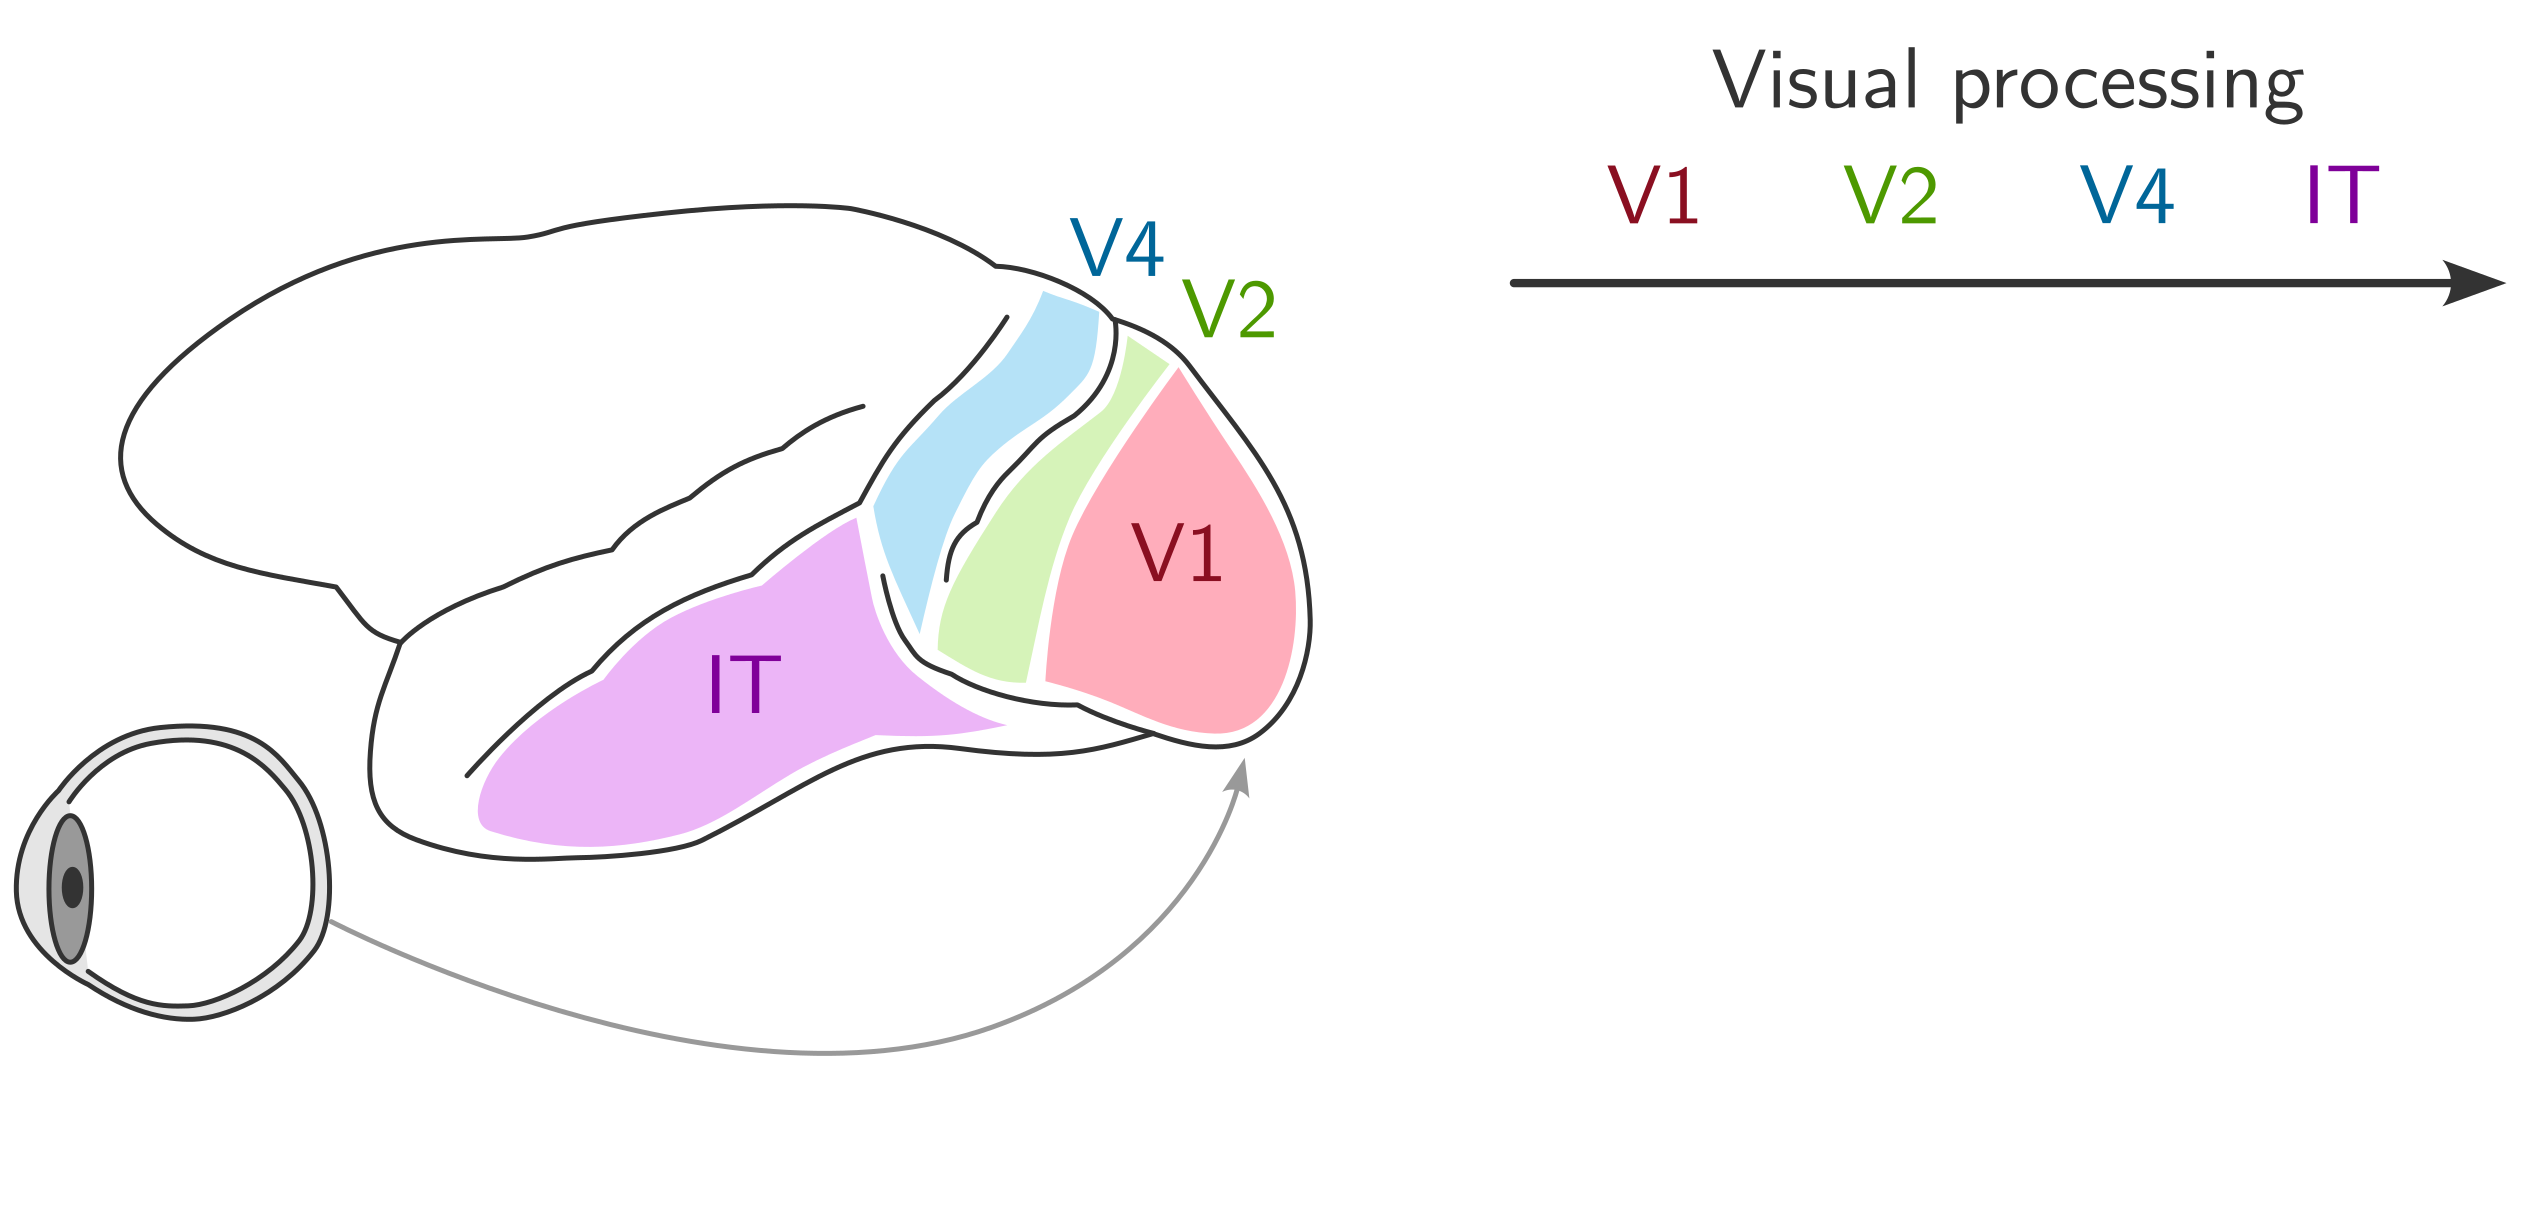
\includegraphics[width=\textwidth]{img/visual_regions-1.png}}
  \only<2| handout:0>{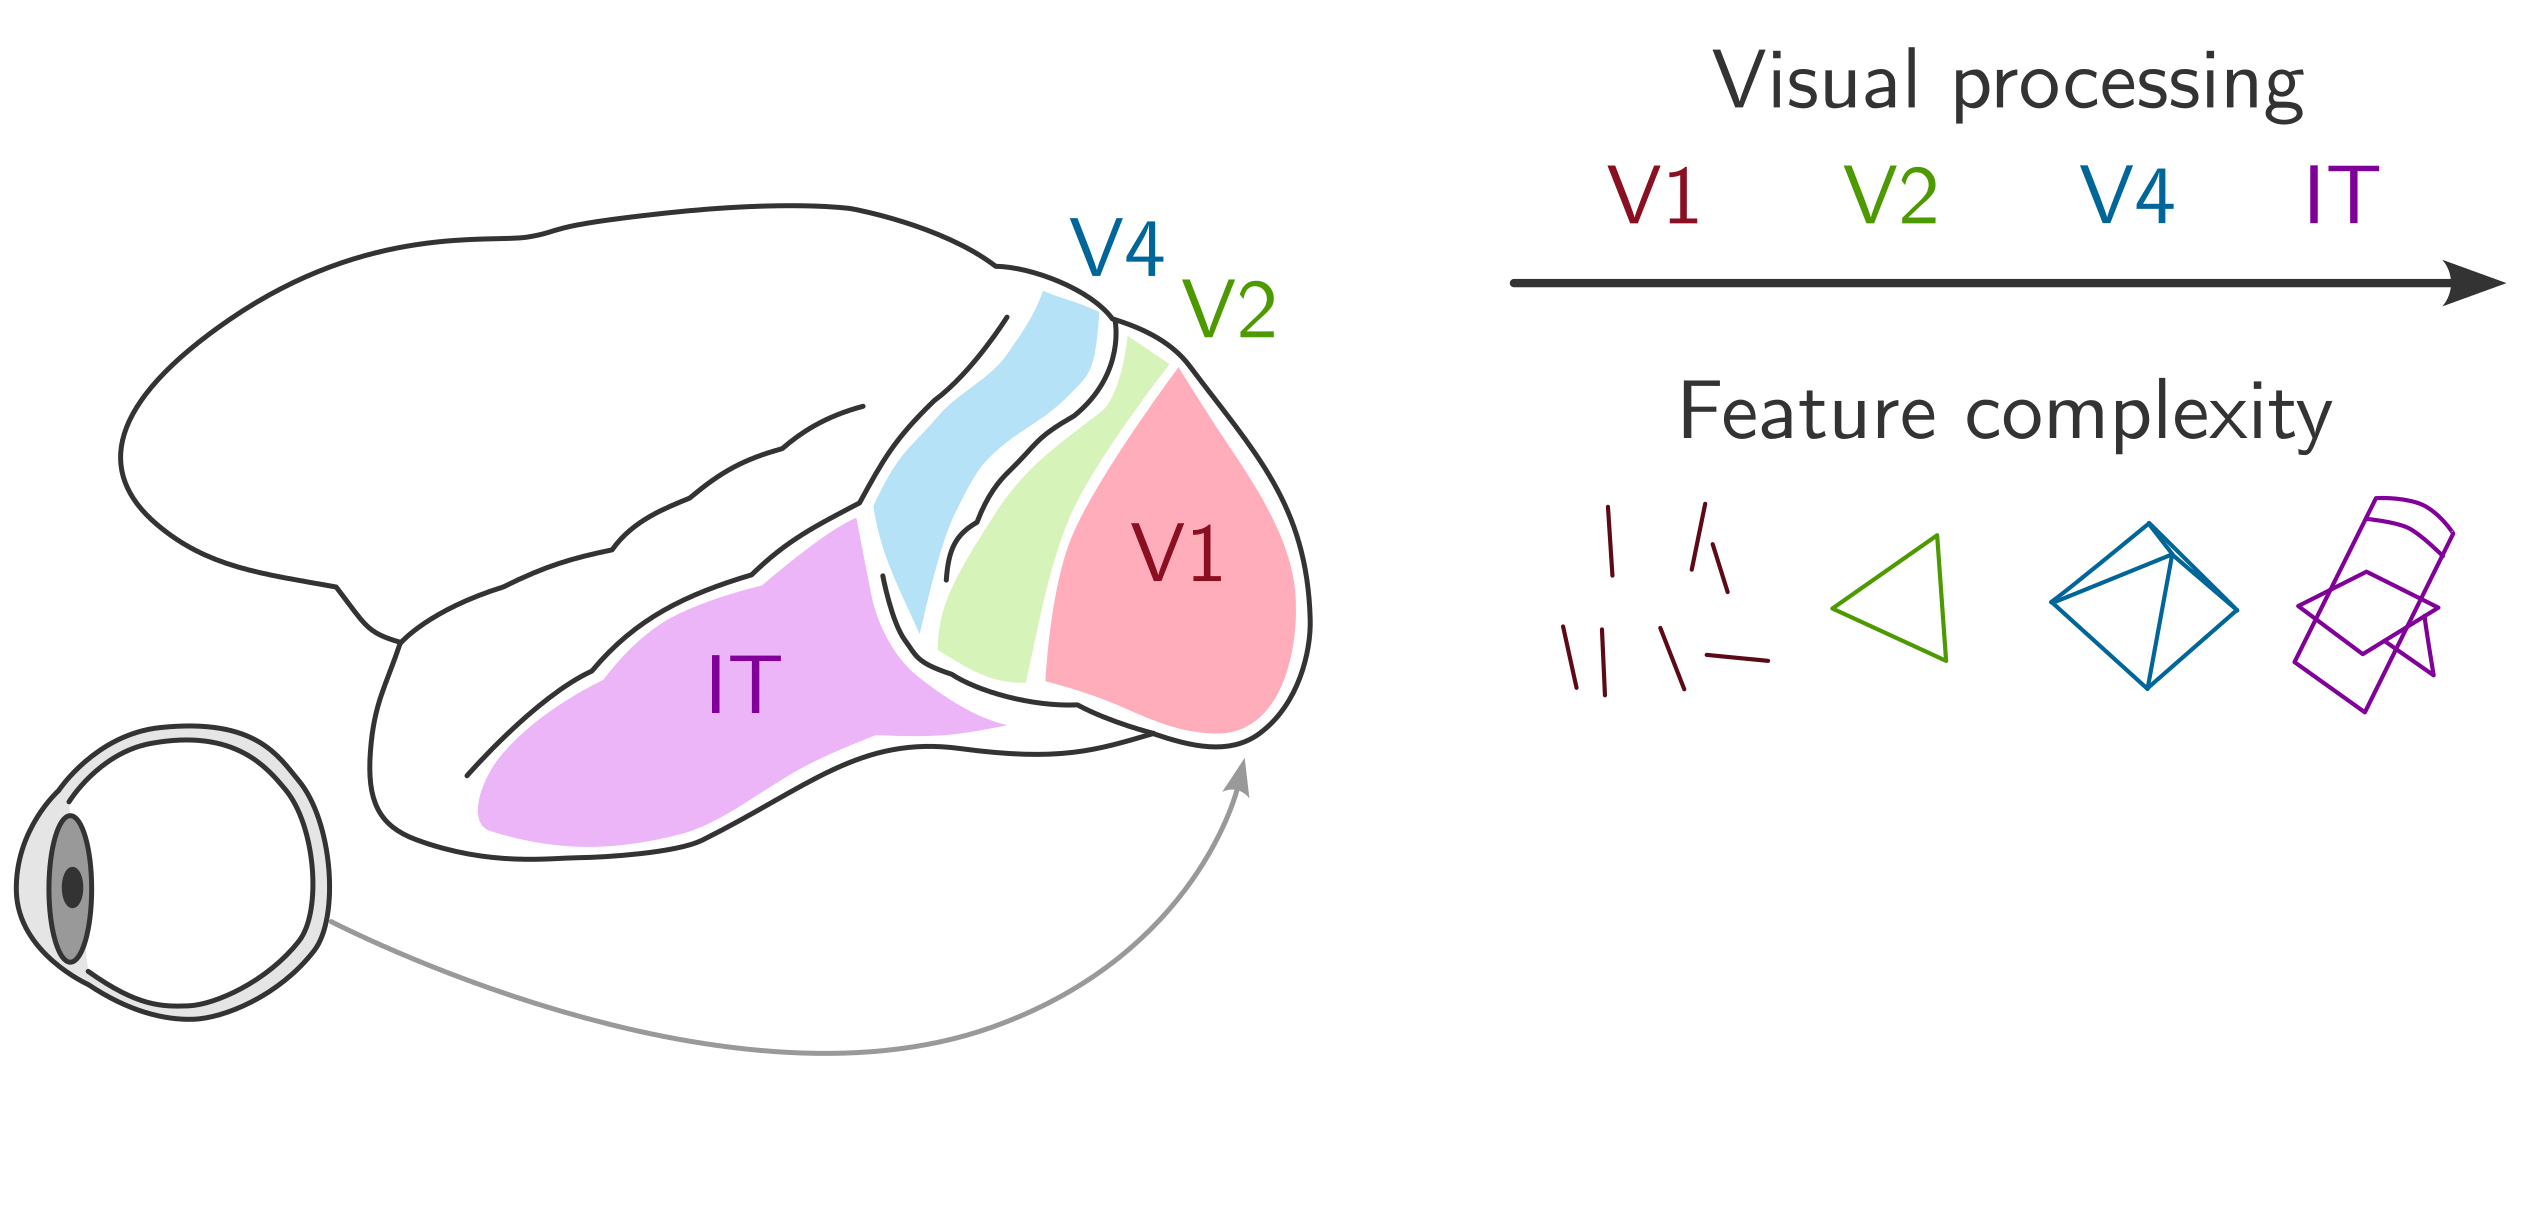
\includegraphics[width=\textwidth]{img/visual_regions-2.png}}
  \only<3| handout:1>{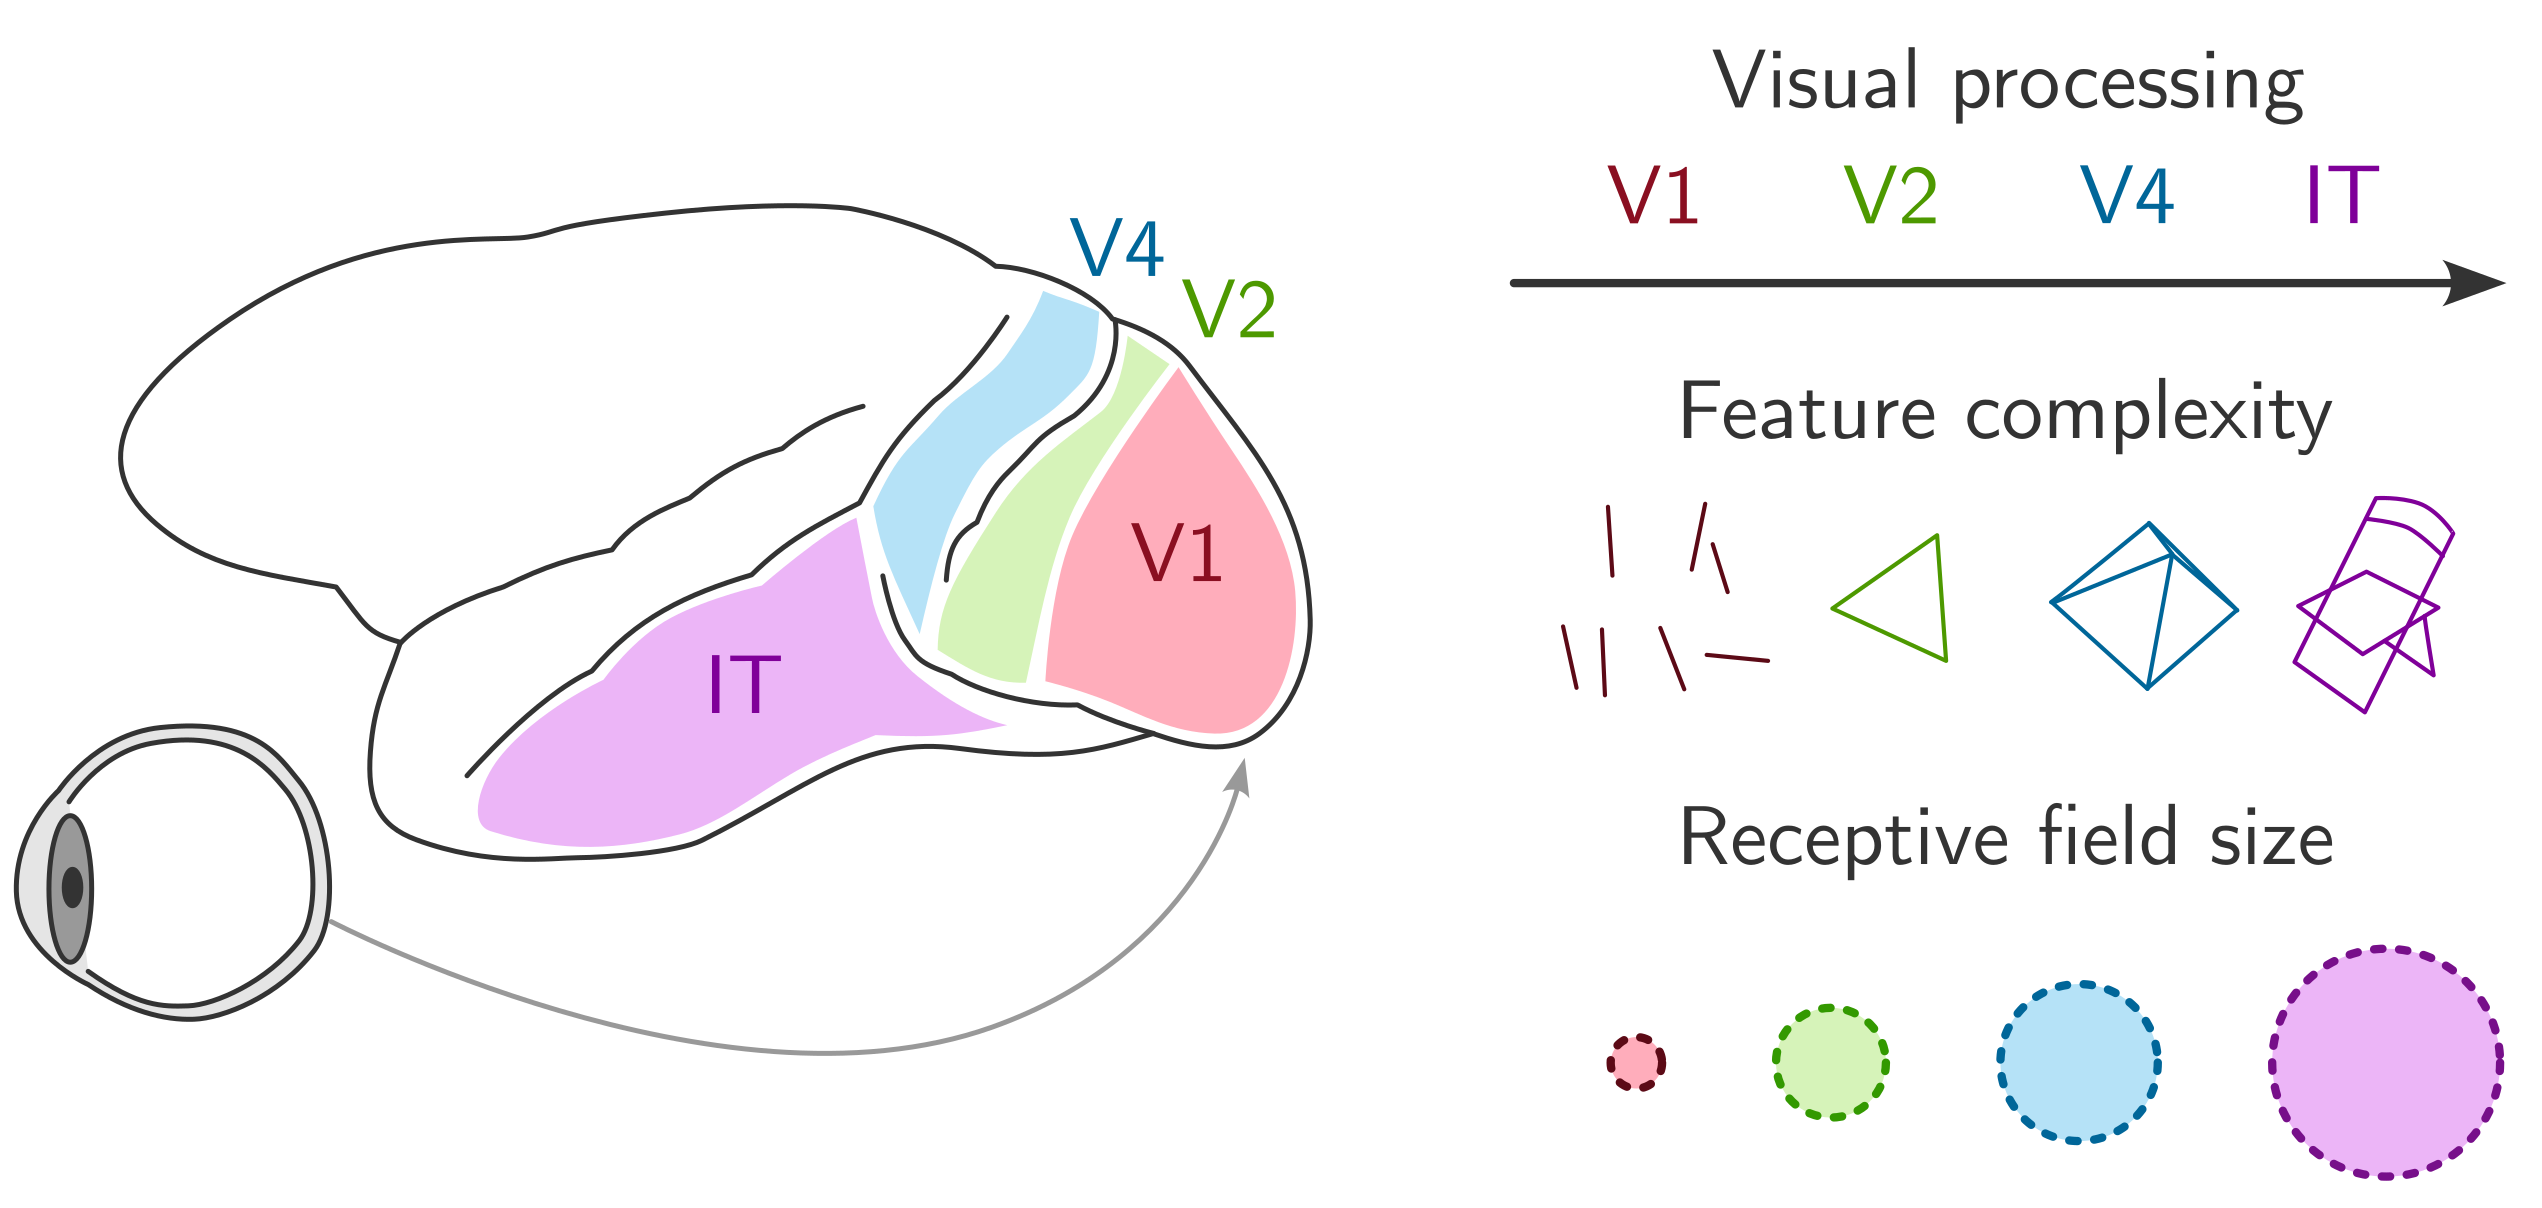
\includegraphics[width=\textwidth]{img/visual_regions-3.png}}
\end{frame}

\begin{frame}{Visual textures can be parameterized  based on higher order image statistics}
\vspace{20pt}
\begin{columns}
    \begin{column}{0.1\textwidth}
    \end{column}
    \begin{column}{0.9\textwidth}
        \centering
        \only<1| handout:0>{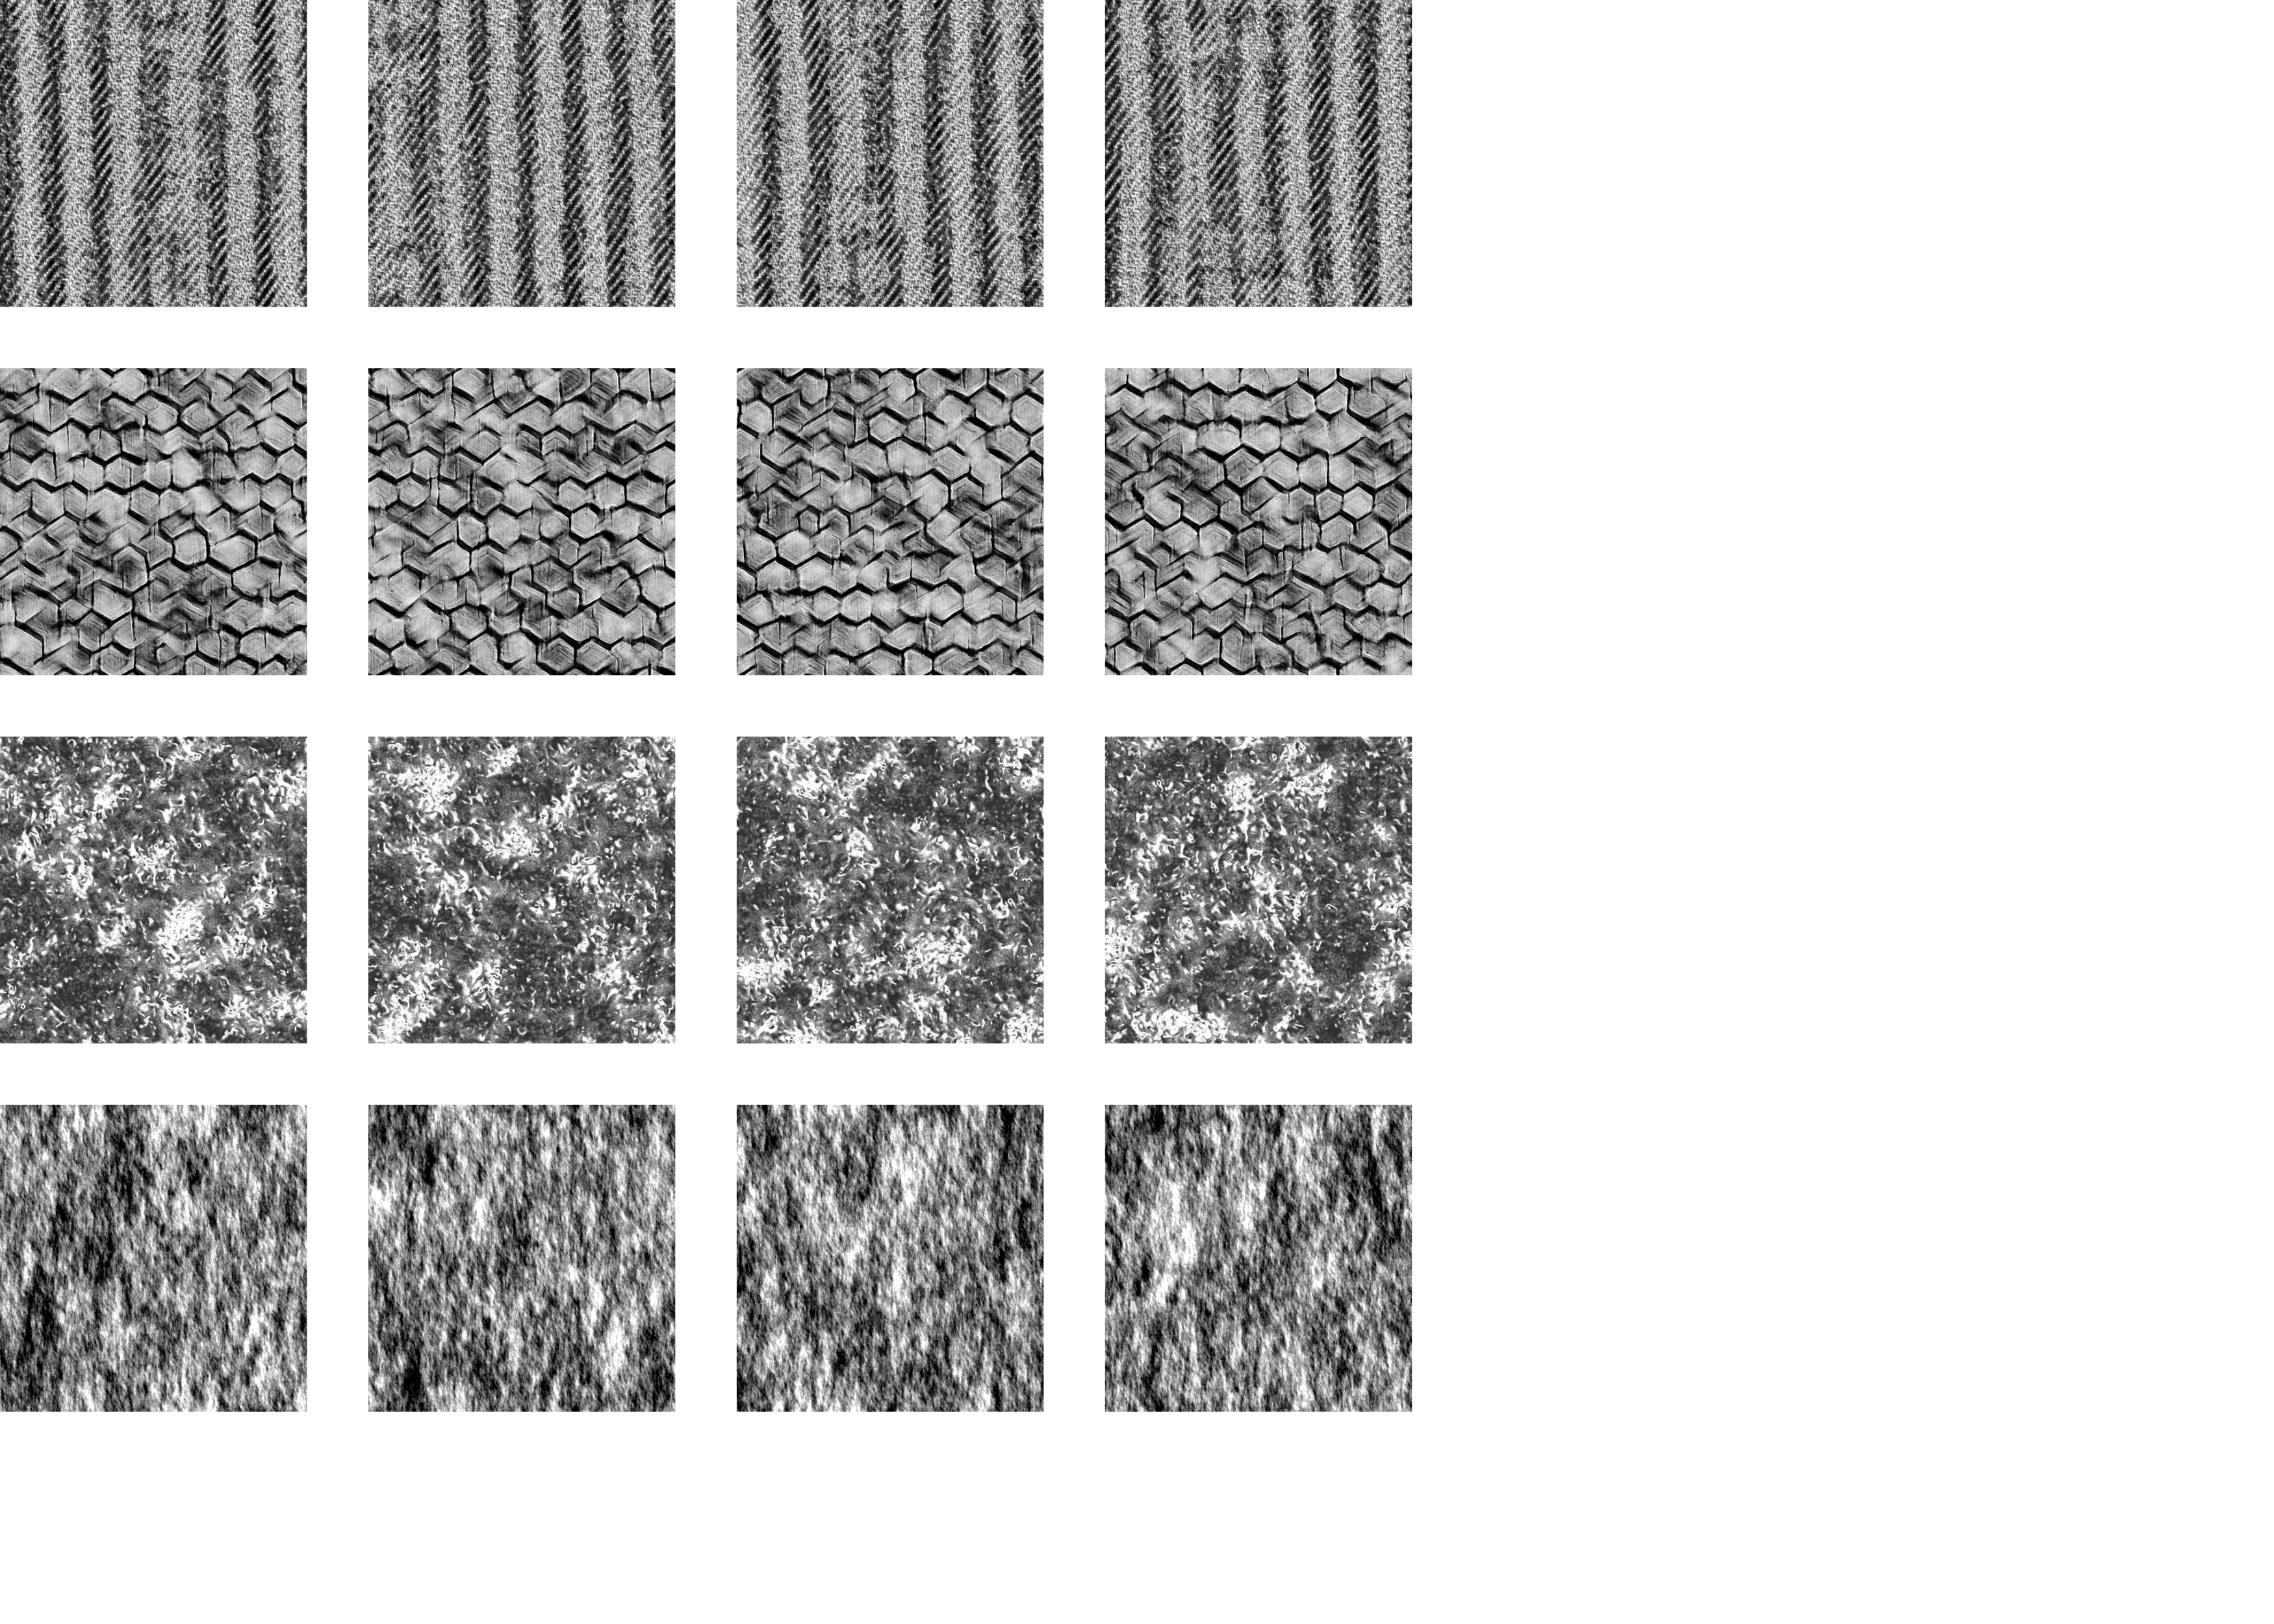
\includegraphics[width=0.8\textwidth]{img/texture_families-1.png}}
        \only<2| handout:0>{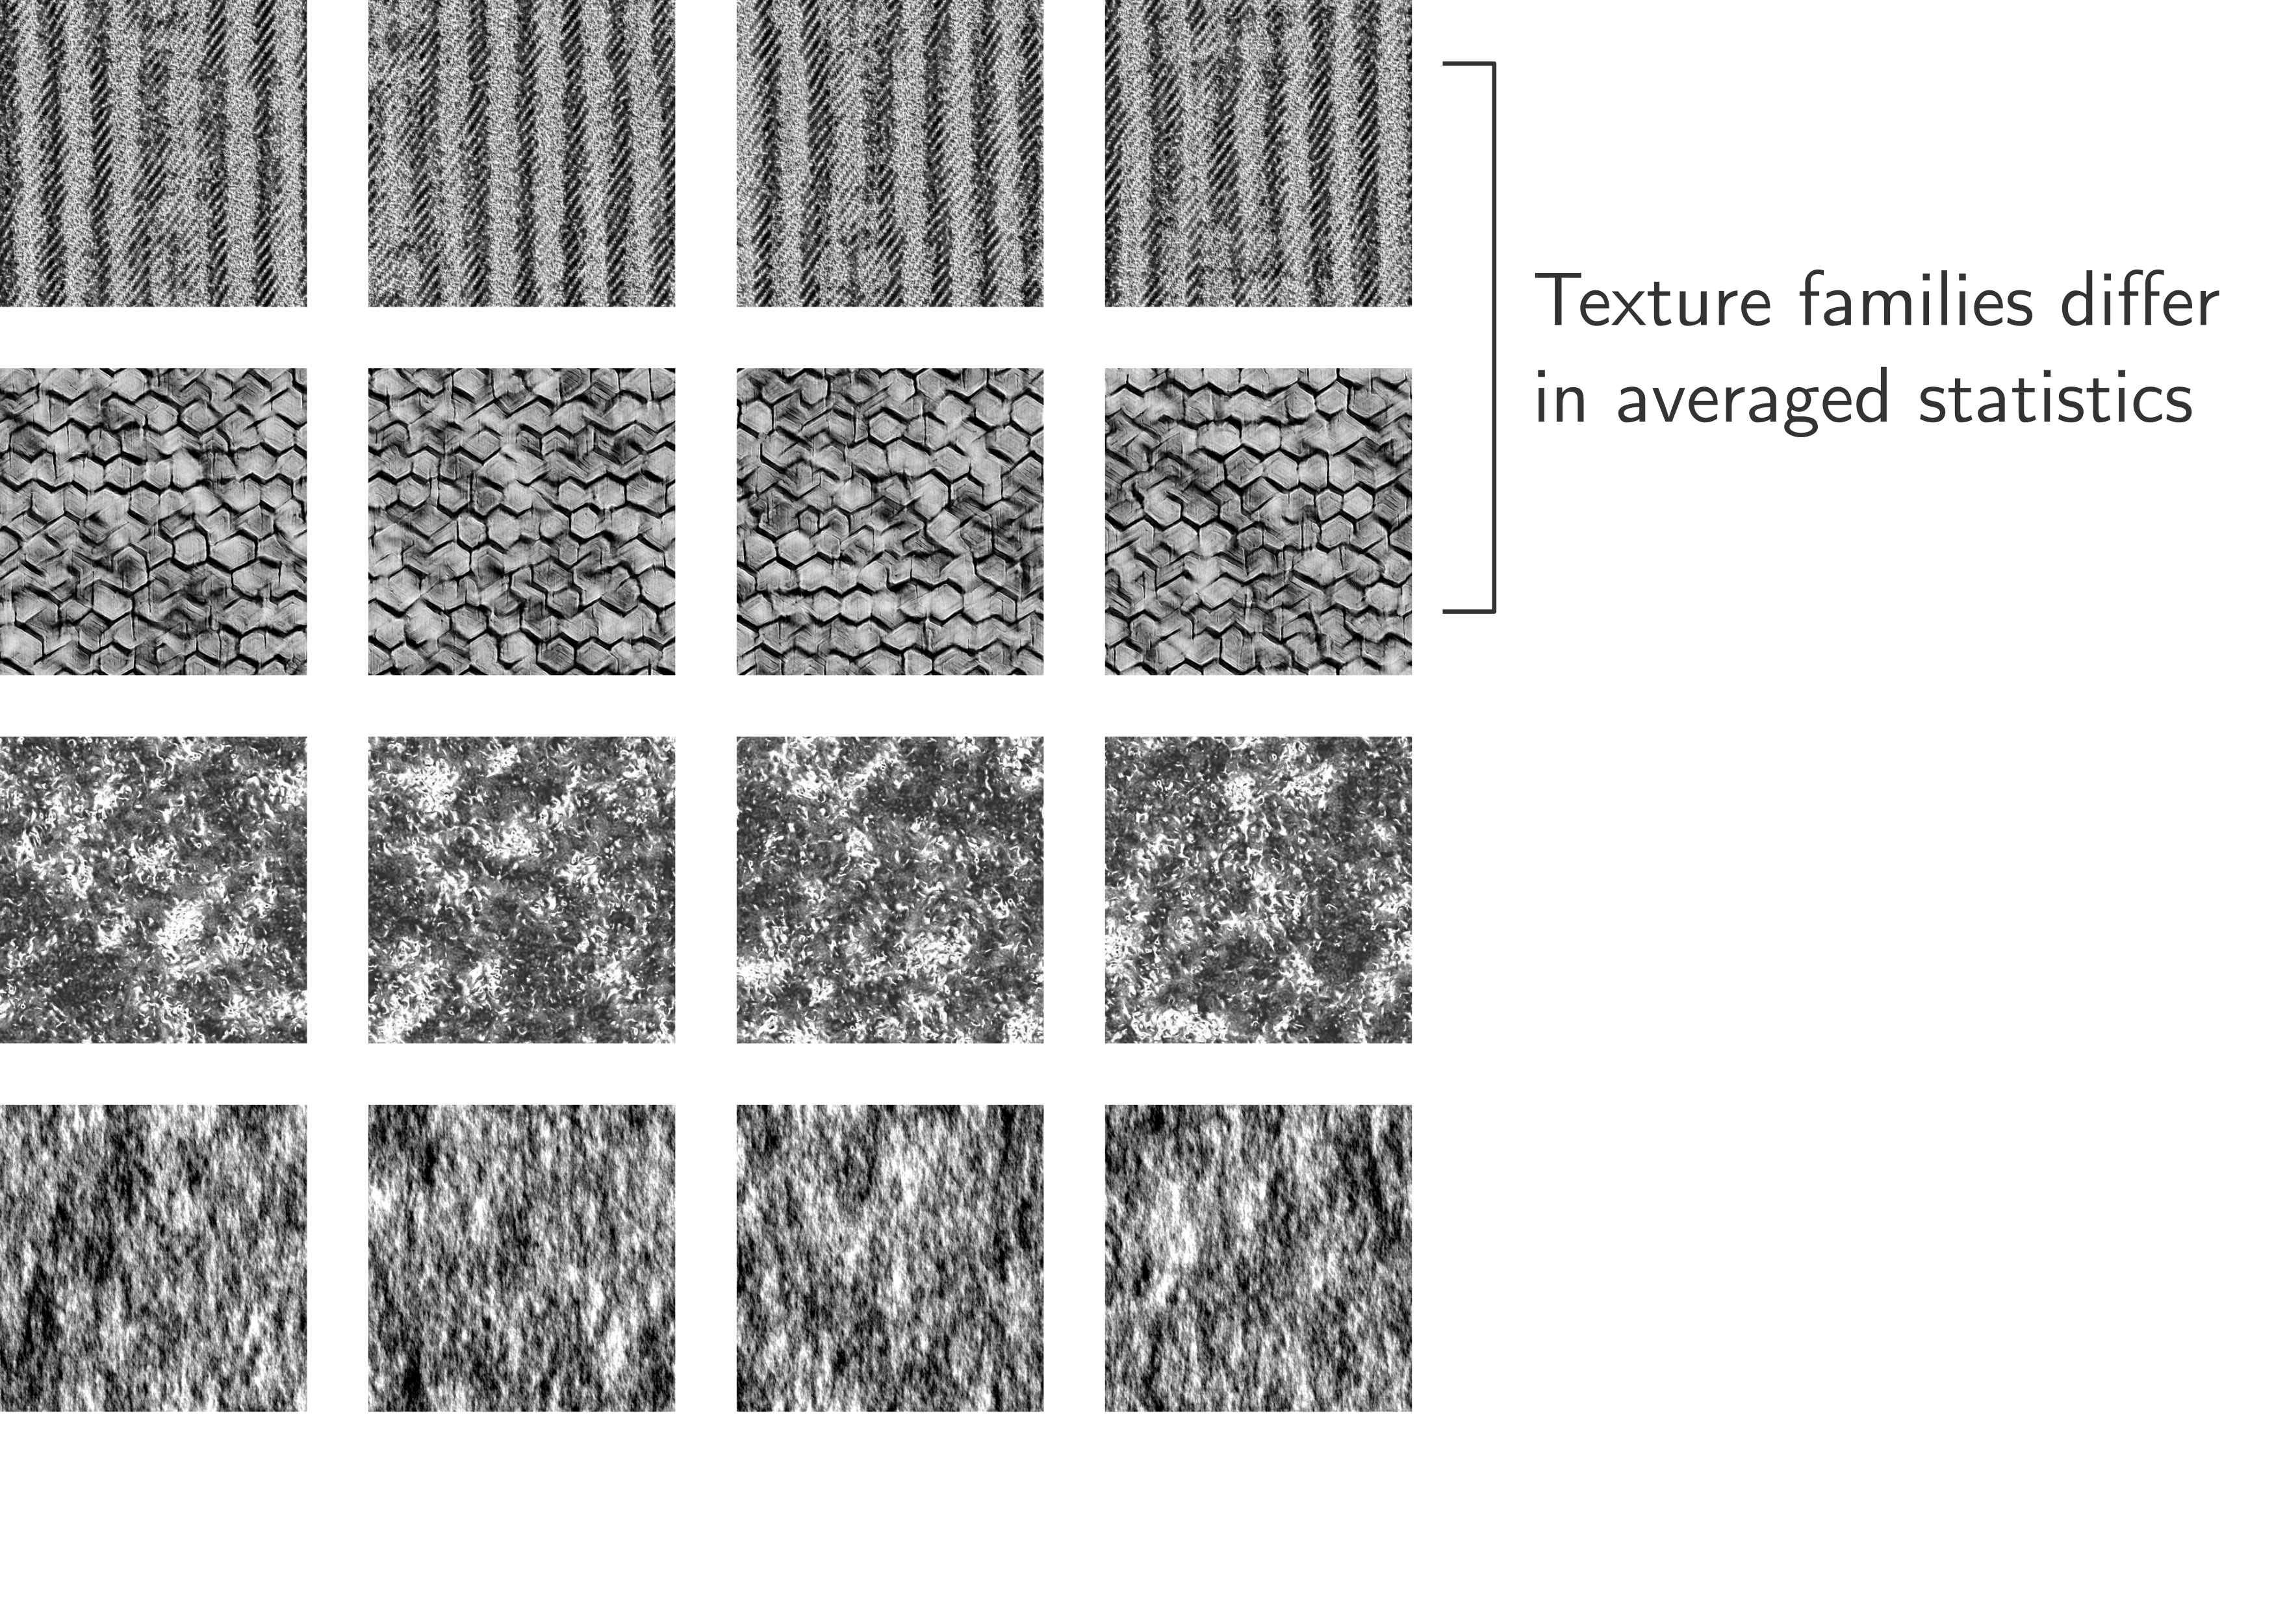
\includegraphics[width=0.8\textwidth]{img/texture_families-2.png}}
        \only<3| handout:1>{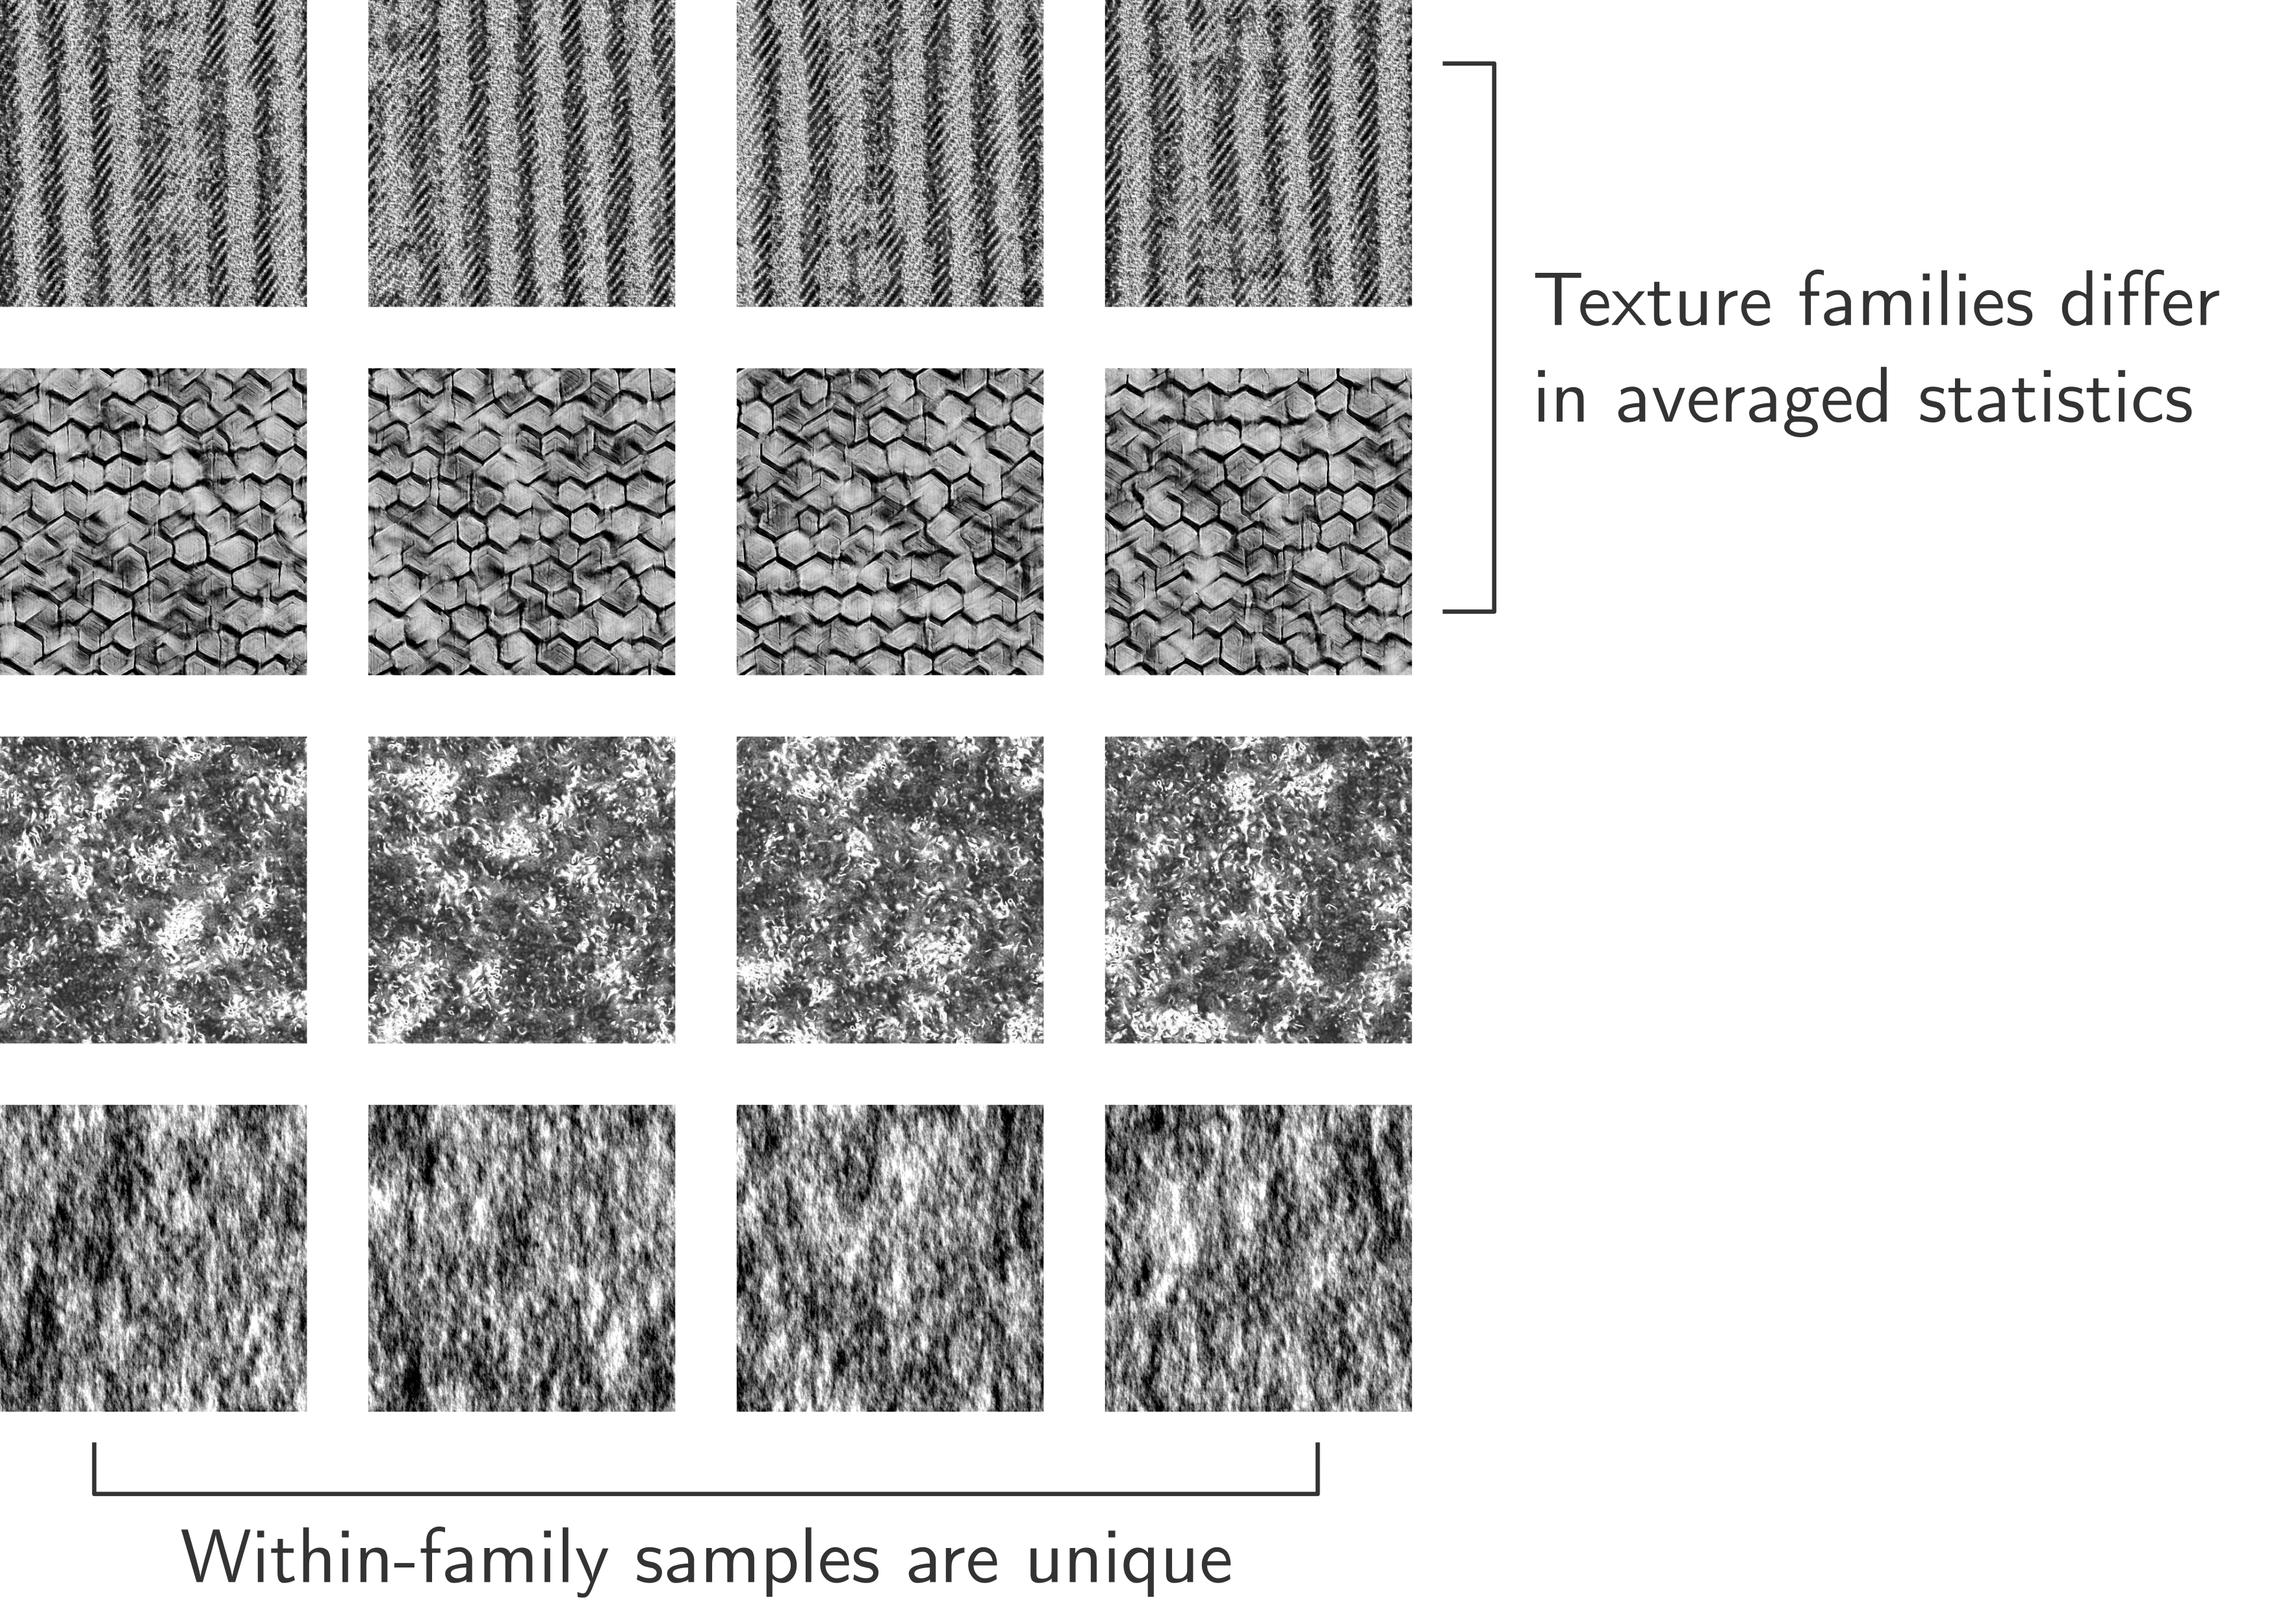
\includegraphics[width=0.8\textwidth]{img/texture_families-3.png}}
    \end{column}
\end{columns}
\end{frame}

\begin{frame}{Separation between families may trade off with separation of samples}
\vspace{10pt}
\centering
\begin{columns}
\begin{column}{0.4\textwidth}
    \centering
    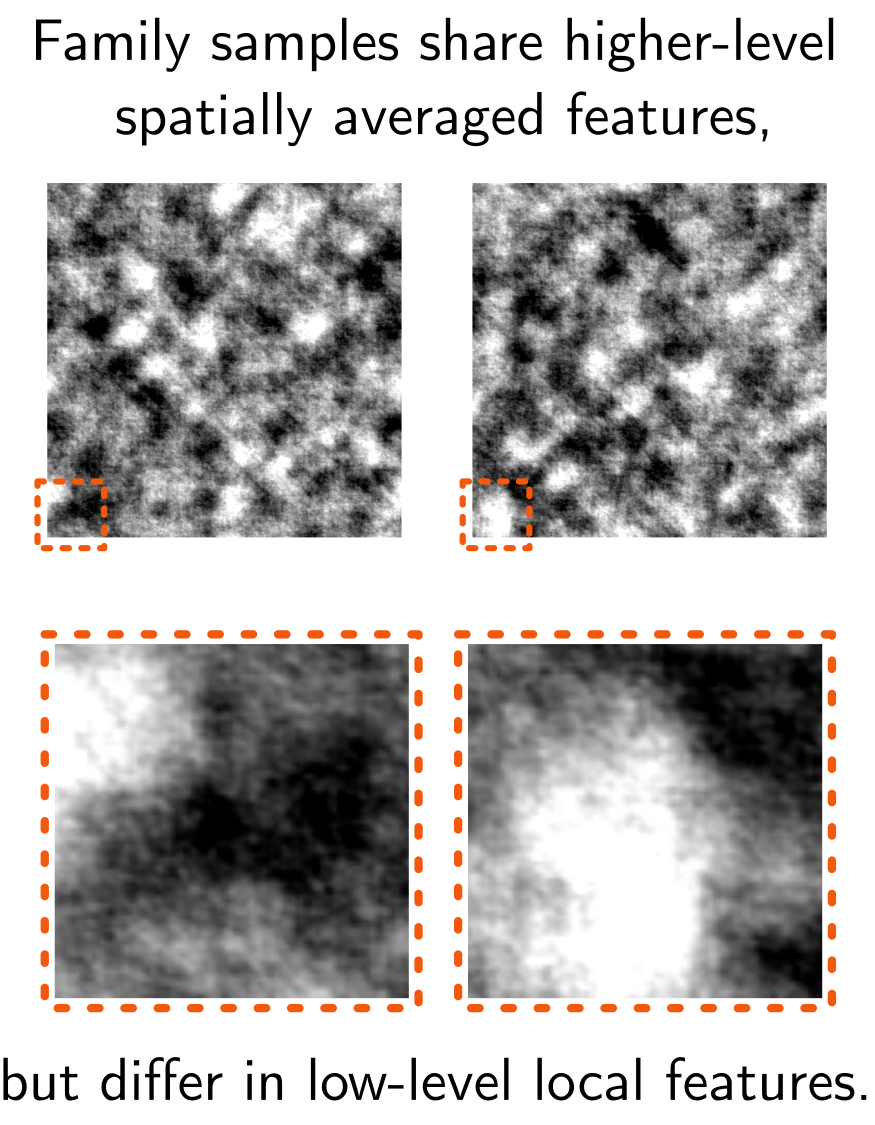
\includegraphics[width=\textwidth]{img/texture_samples-2.png} \pause 
\end{column}
\begin{column}{0.6\textwidth}
    \begin{center}
    We expect the following trends in separability: 
    
    \vspace{10pt}

    \centering 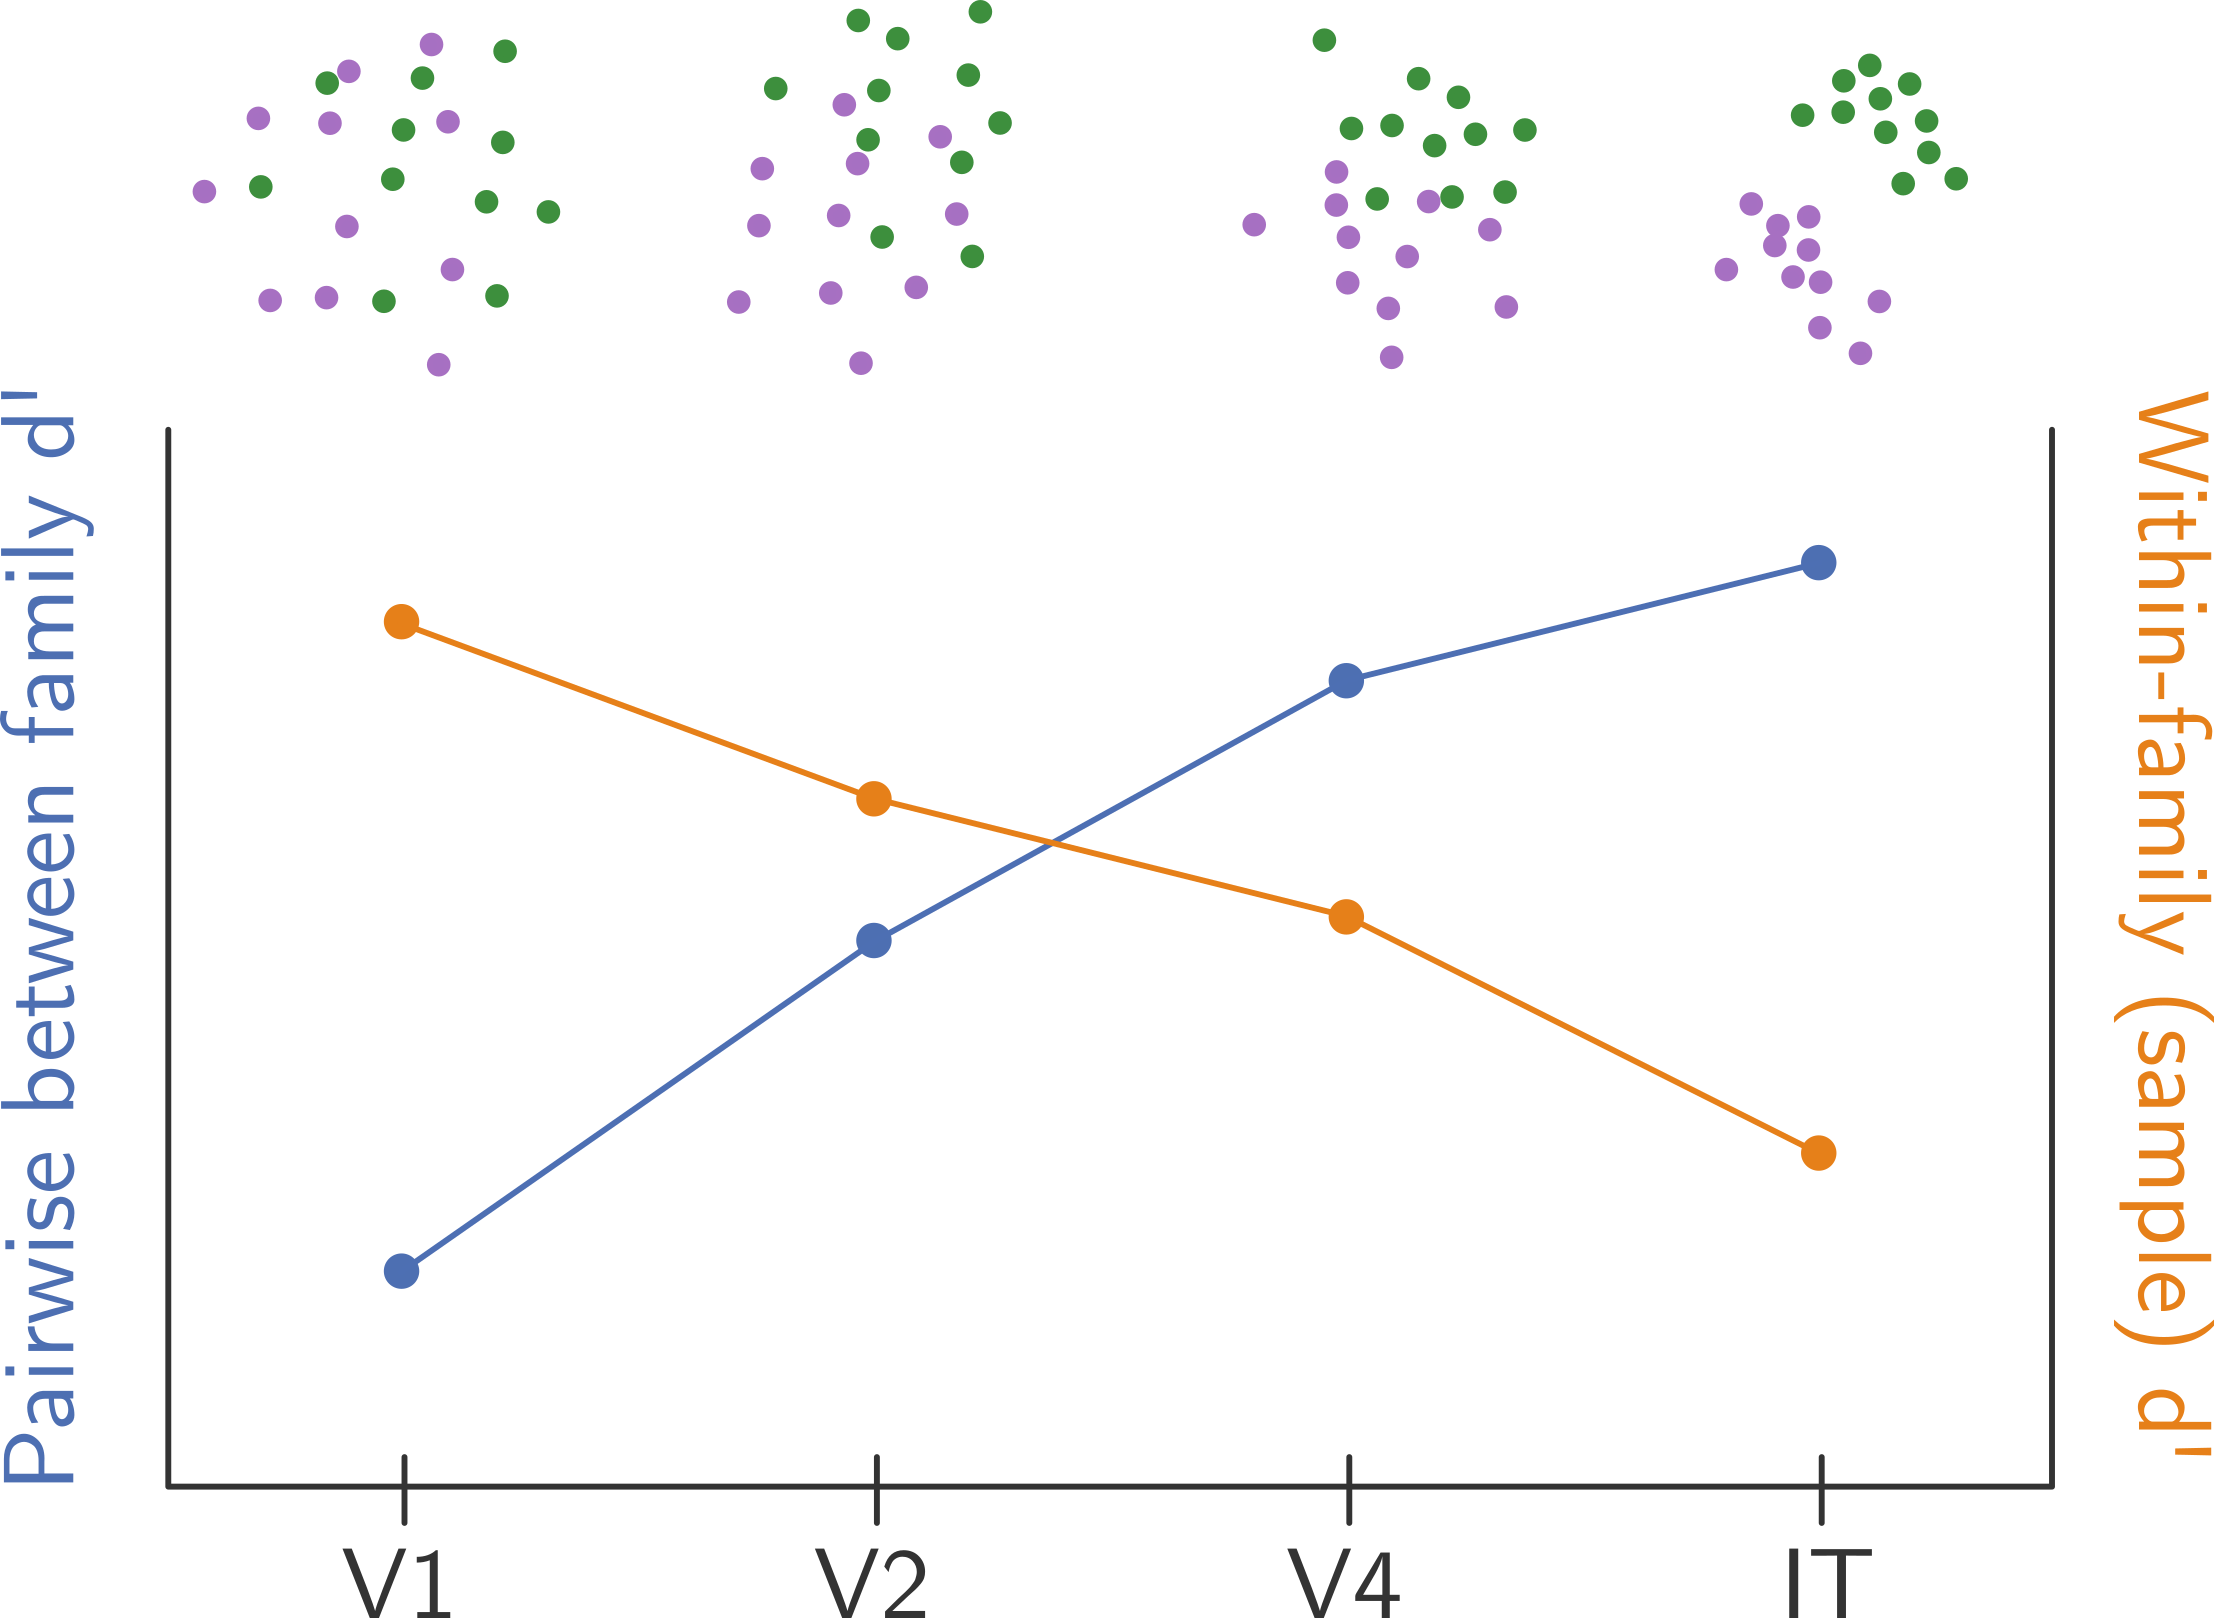
\includegraphics[width=0.6\textwidth]{img/proposed_results.png} \pause 
    \end{center}
    
    \begin{itemize}
    \item The expected trend has been shown in V2 vs. V1 and V4 vs. V2 \parencite{ziemba_selectivity_2016, okazawa_gradual_2017} \pause 
    \item Neither covers the entire hierarchy
\end{itemize}
\end{column}
\end{columns}
\end{frame}

\section{Data}

\begin{frame}{Six subjects were implanted with \( \approx \)two arrays each, producing uneven samples of multi-unit activations between regions}
  \centering
  \only<1| handout:0>{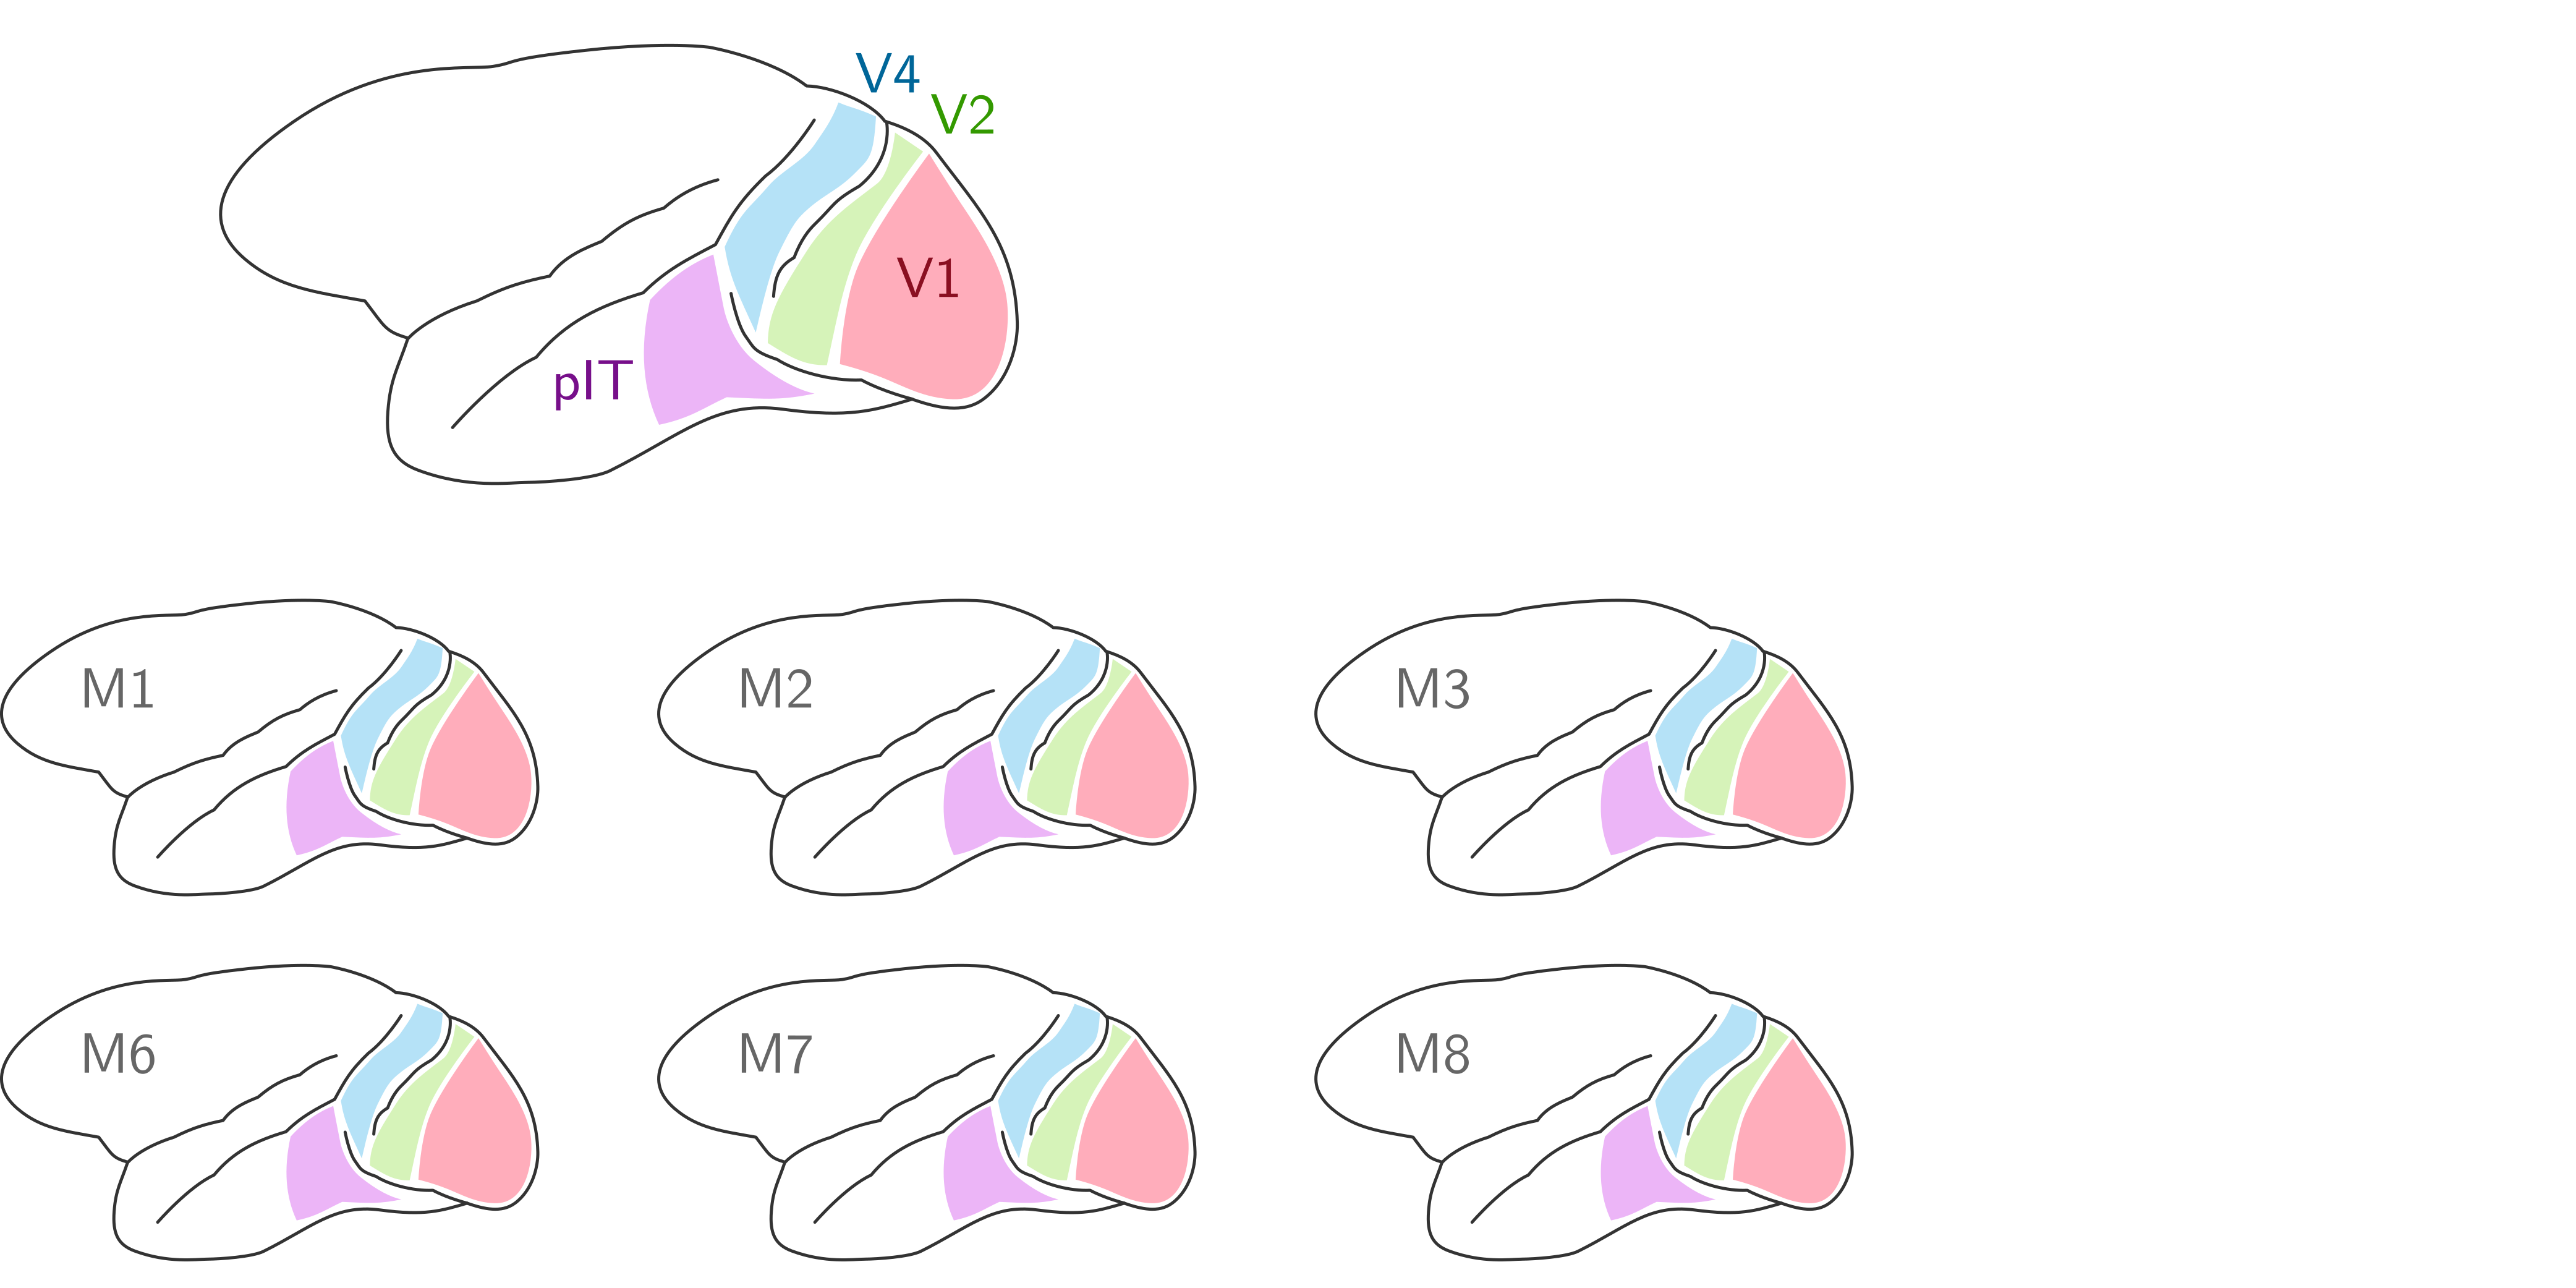
\includegraphics[width=\textwidth]{img/array_locations-1.png}}
  \only<2| handout:0>{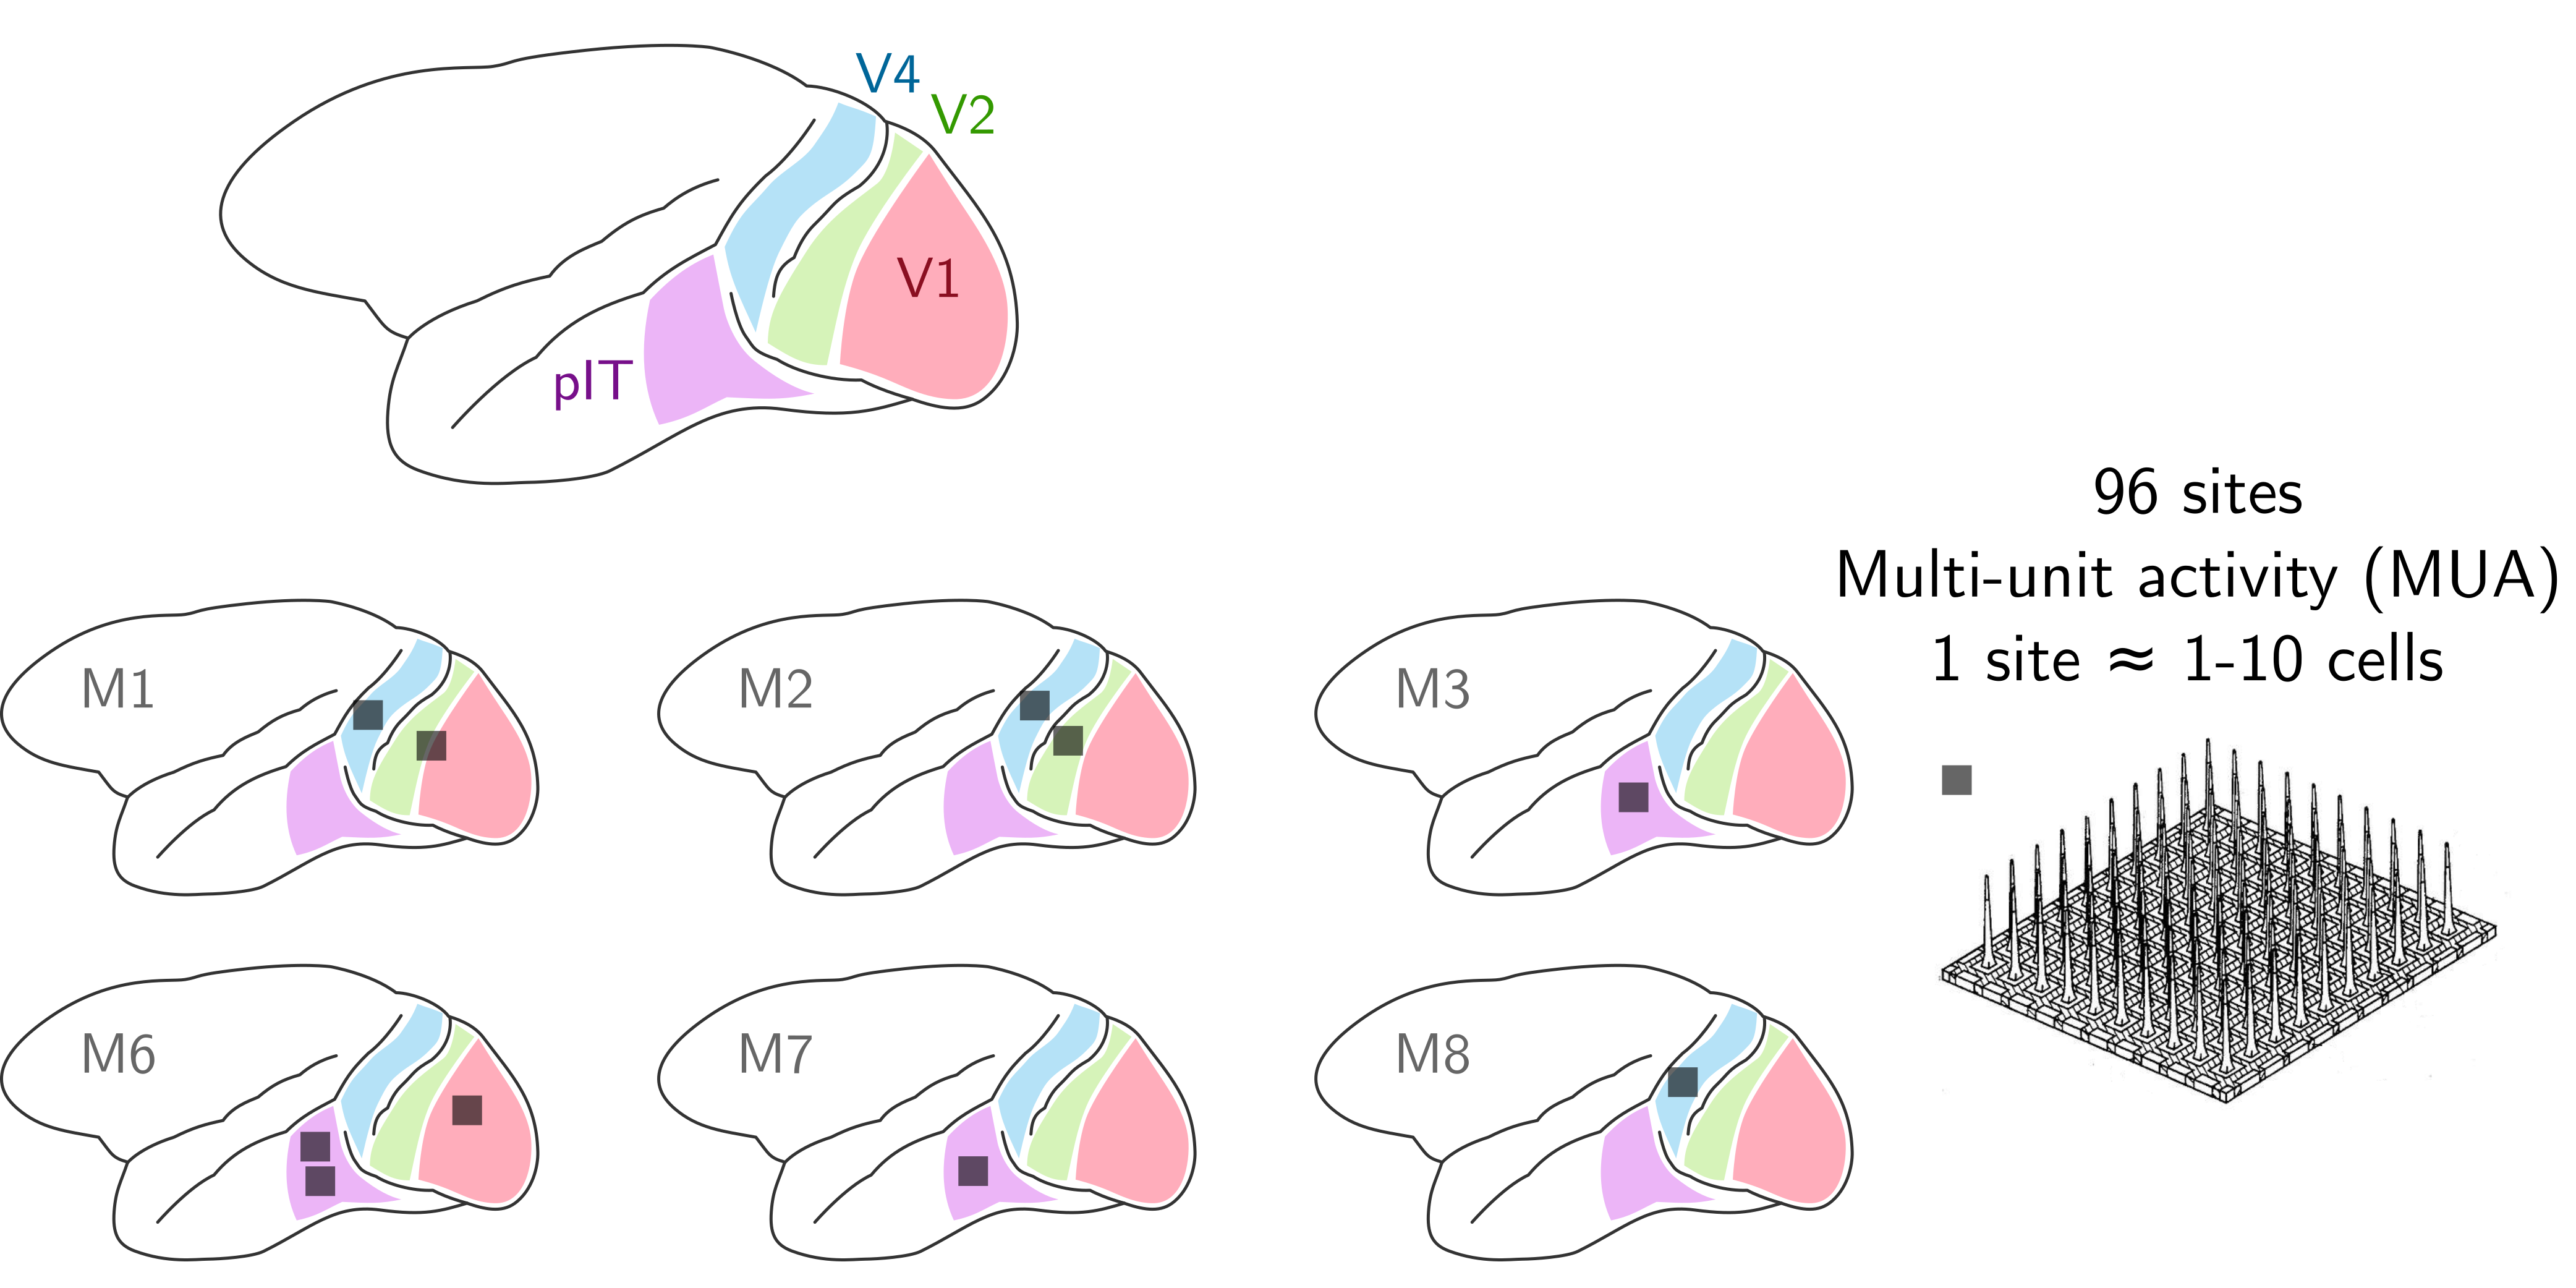
\includegraphics[width=\textwidth]{img/array_locations-2.png}}
  \only<3| handout:1>{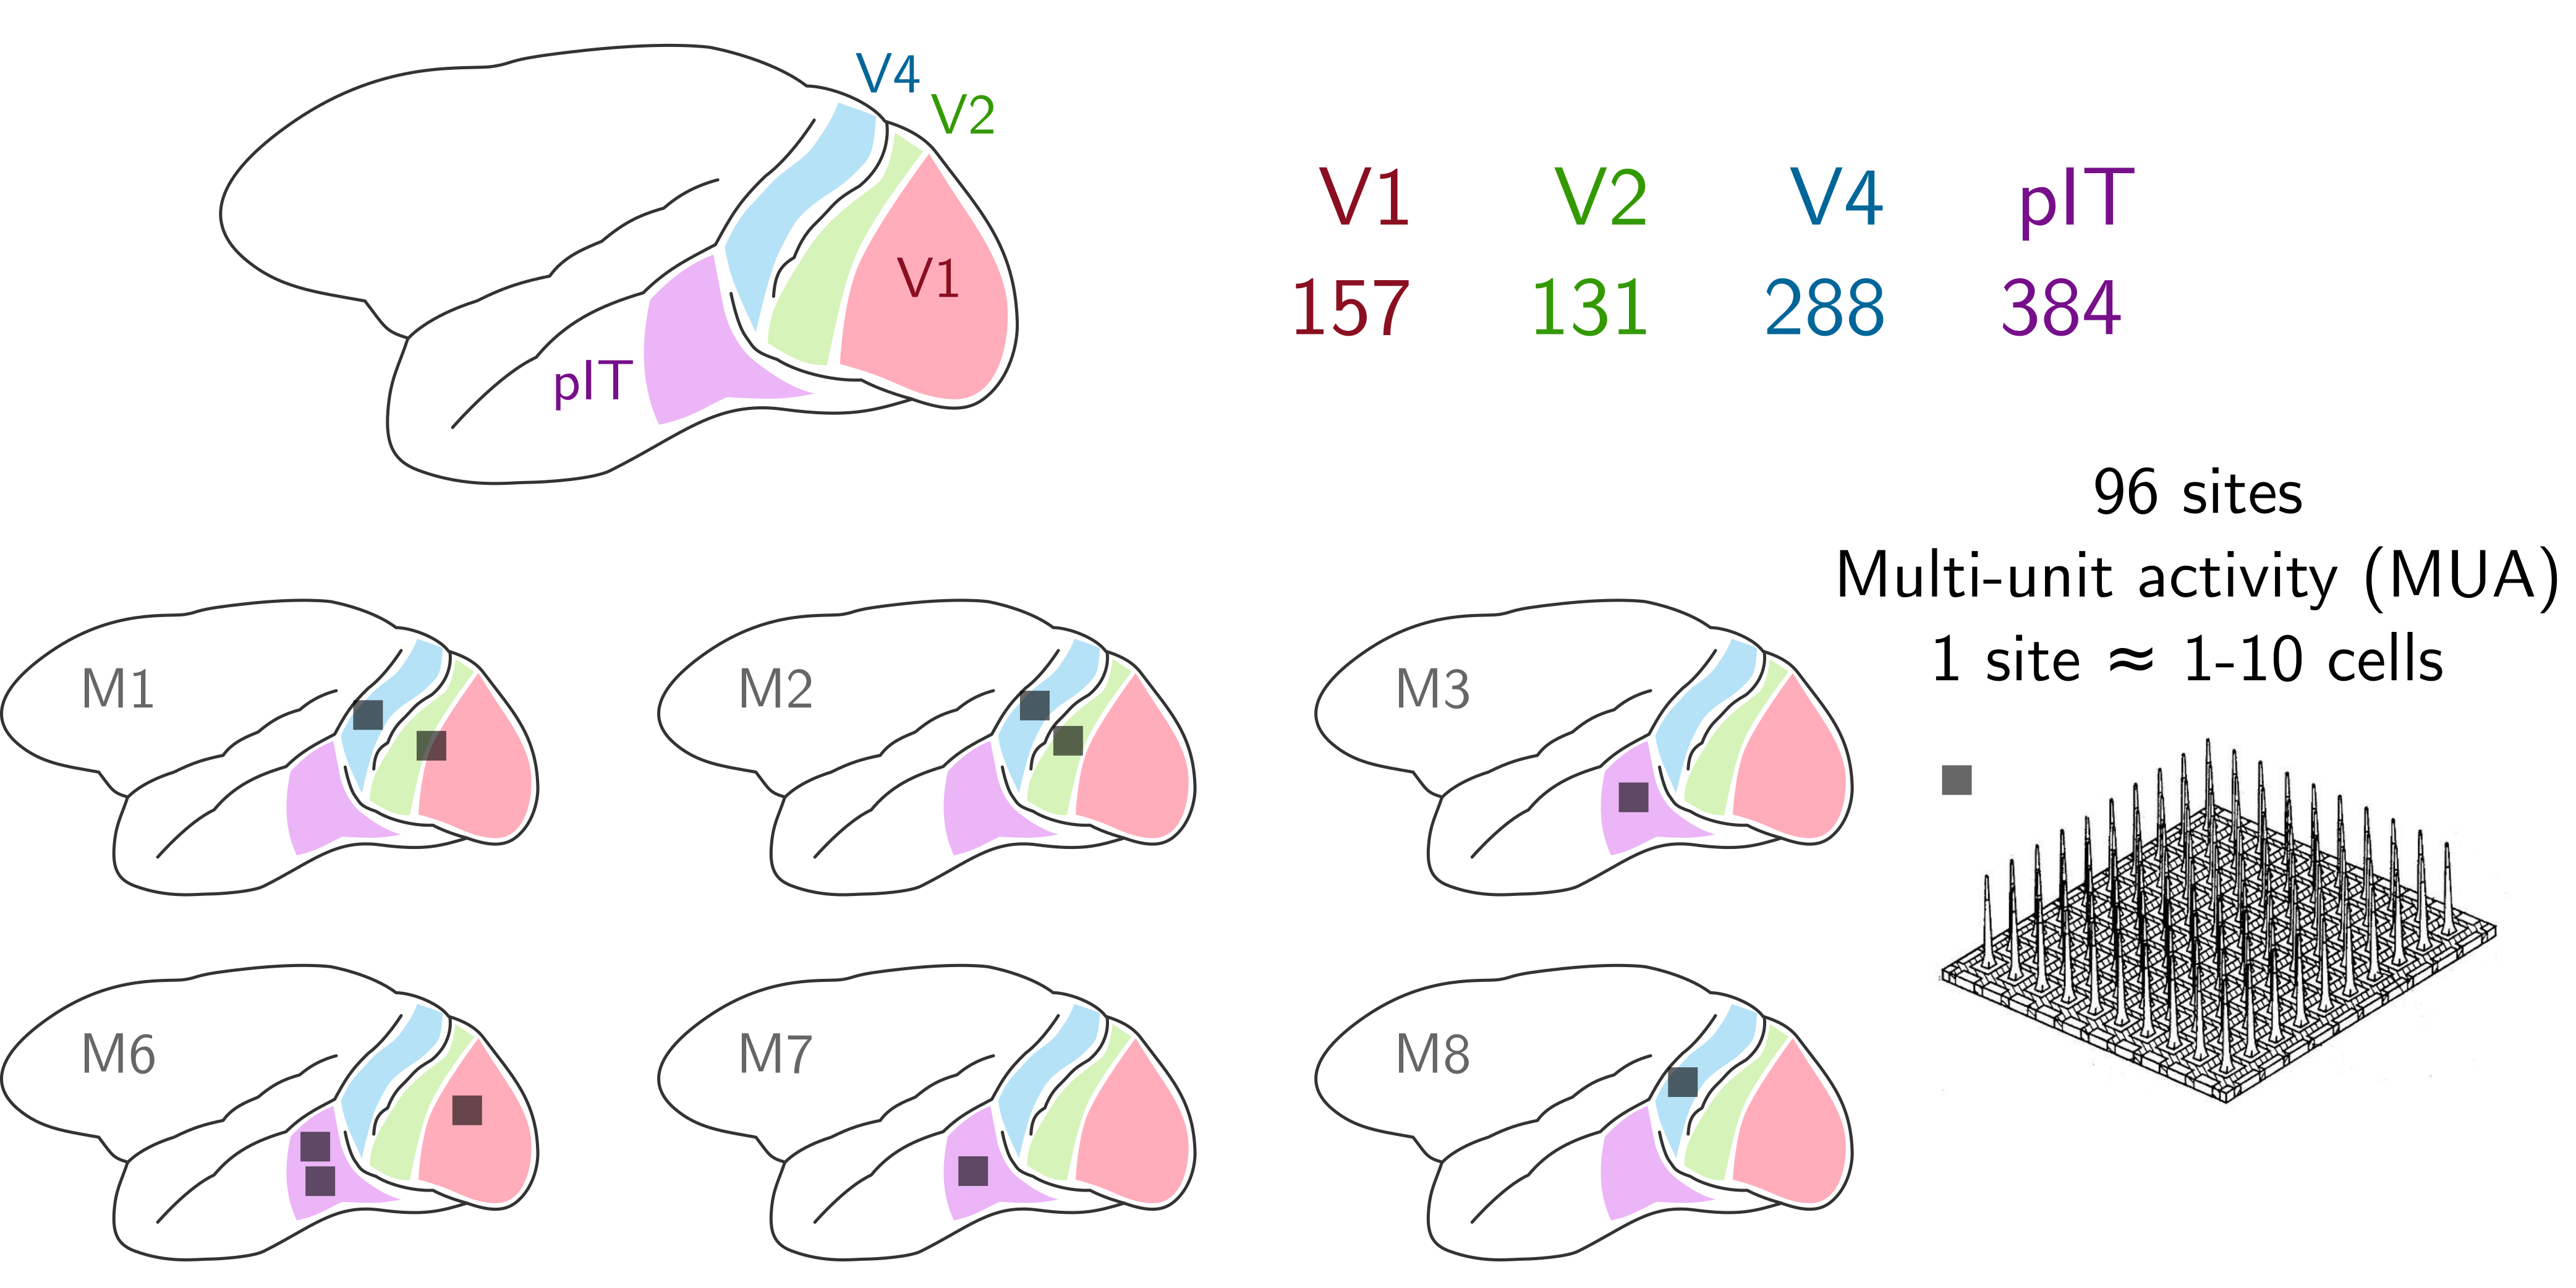
\includegraphics[width=\textwidth]{img/array_locations-3.png}}
\end{frame}

\begin{frame}{Neural recordings taken during passive fixation}

\centering
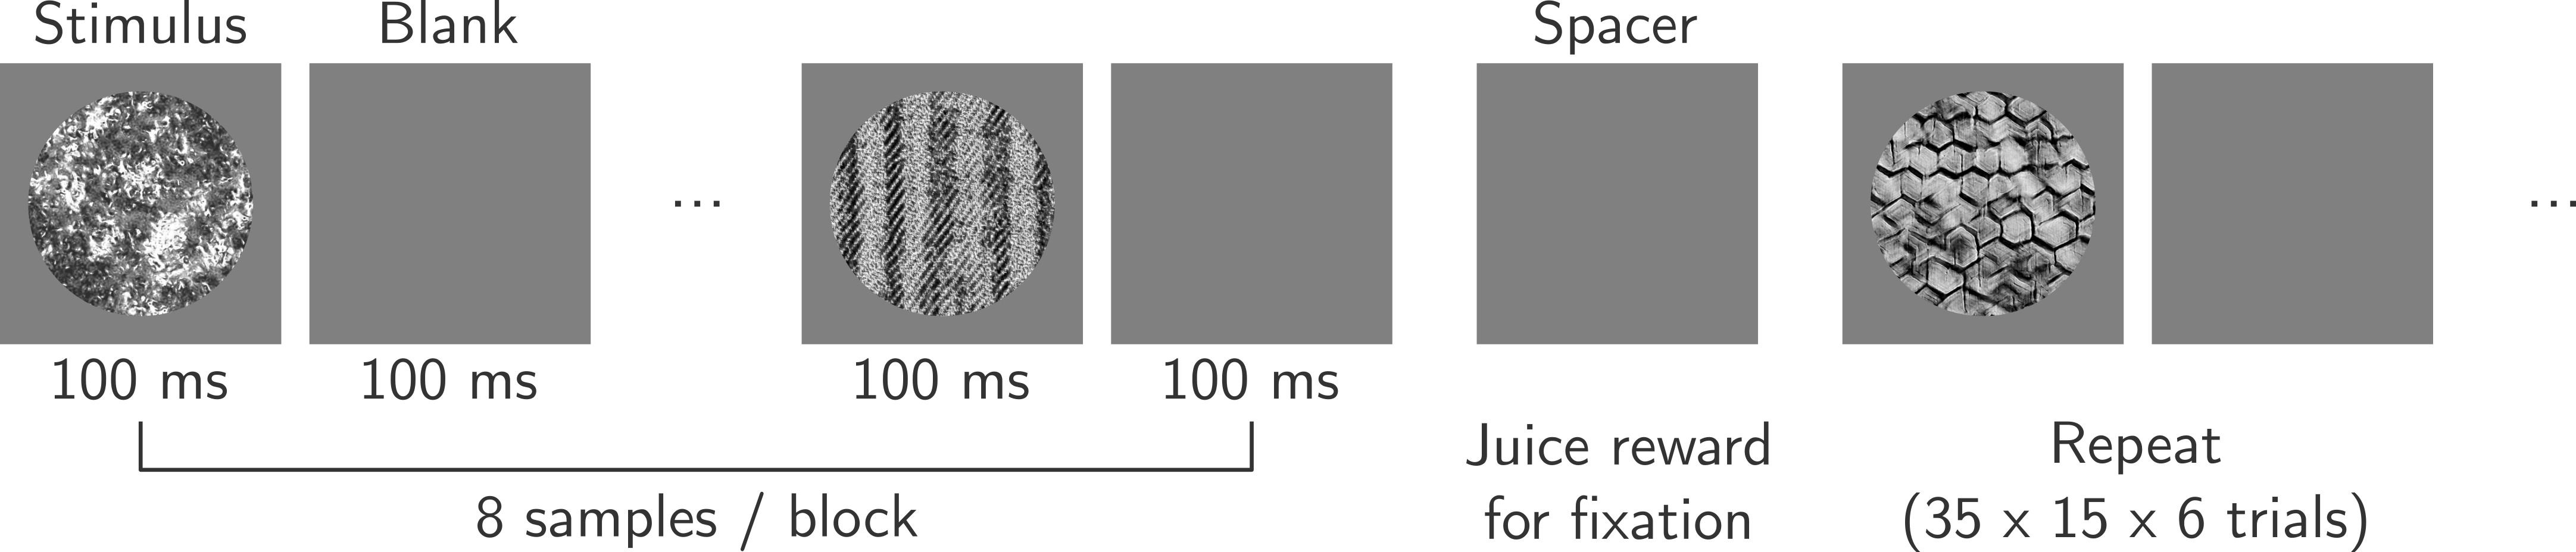
\includegraphics[width=\textwidth]{img/passive_fixation.png} 
\pause 
\begin{itemize}
    \item \parencite{lee_developmentally_2024} 35 families, 15 samples per family, and 6 repetitions \pause  
    \item 100 x 6 blanks stimuli per session, interspersed within blocks
\end{itemize}
\end{frame}

% \begin{frame}{Road map}
% \begin{enumerate}
%     \item Regions higher in the visual hierarchy show higher sparsity.
%     \item Sparsity and reliability are linked, and reliability influences downstream summaries.
%     \item Reliability-based balancing finds IT between-family separability to be comparable to V4.
%     \item Within-family between-sample separability is lower in V4 and IT compared to V1 and V2. 
% \end{enumerate}
% \end{frame}

\section{Methods}

\begin{frame}{Approach}
    \begin{enumerate}
        \item Define a model of neural separability \pause 
        \item Identify inter-region differences that affect separability estimation \pause 
        \item Correct for regional differences to produce comparable separability estimates
    \end{enumerate}
\end{frame}

\begin{frame}{Approach}
    \begin{enumerate}
        \item Define a model of neural separability
        \color{gray} \item  Identify inter-region differences that affect separability estimation 
        \color{gray} \item  Correct for regional differences to produce comparable separability estimates
    \end{enumerate}
\end{frame}

\begin{frame}{Model of texture family separation in neural responses}
\[ y_{f, s, r} = \mu + a_f + b_{s(f)} + c_r + \epsilon_{f, s, r} \]
\begin{itemize}
    \item \( y_{f, s, r} \): \hl{per-site} firing on family \( f \), sample \( s (f) \), and replication \( r \). \pause  
    \item \( \mu \): baseline firing (to blank stimuli). \pause 
    \item \( a_f, b_{s(f)}, c_r \): level effects of family, sample (nested), and replication. \pause 
    \item \( \epsilon_{f, s, r }\): trial-specific noise. 
\end{itemize}
\begin{align*}
\begin{bmatrix} 
y_{f, s, r, 1} \\ 
% y_{f, s(f), r, 2} \\
\vdots \\
y_{f, s, r, p} 
\end{bmatrix} = \mathbf{y}_{f, s, r} &= \bfs{\mu} + \mathbf{a}_f + \mathbf{b}_{s(f)} + \mathbf{c}_r + \bfs{\epsilon}_{f, s, r}
\end{align*}
\begin{itemize}
    \item \( \mathbf{y}_{f, s, r} \): firing for a \hl{population} of \( p \) sites 
\end{itemize}
\end{frame}

\begin{frame}{Model of texture family separation in neural responses}
\begin{align*}
\mathbf{y}_{f, s(f), r} &= \bfs{\mu} + \mathbf{a}_f + \mathbf{b}_{s(f)} + \mathbf{c}_r + \bfs{\epsilon}_{f, s(f), r} 
\end{align*}
\begin{itemize}
    \item \( d_M: \mathbb{R}^p \times \mathbb{R}^p \to \mathbb{R} \): multivariate Mahalanobis distance \pause 
    \item \( d_M (\mathbf{x}, \mathbf{y}) = \sqrt{(\mathbf{x} - \mathbf{y})^\top \bfs{\Sigma}^{-1} (\mathbf{x} - \mathbf{y})^\intercal }\) \pause 
    \item \( = \| \mathbf{S}^{-1} (\bfx - \bfy) \|: \pmb\Sigma = \mathbf{S}^\intercal \mathbf{S}\)  (Euclidean distance after whitening) \pause 
\end{itemize}
\begin{align*} 
% & d_M (\bfs{\mu} + \mathbf{a}_{f_1}, \bfs{\mu} \mathbf{a}_{f_2} )  &  \textrm{(family-wise)} \\
% & d_M (\bfs{\mu} + \mathbf{a}_f + \mathbf{b}_{s_1 (f)}, \bfs{\mu} + \mathbf{a}_f + \mathbf{b}_{s_2 (f)}) & \textrm{(sample-wise)} 
& d_M ( \mathbf{a}_{f_1},  \mathbf{a}_{f_2} )  &  \textrm{(family-wise)} \\
& d_M (\mathbf{b}_{s_1 (f)}, \mathbf{b}_{s_2 (f)}) & \textrm{(sample-wise)} 
\end{align*}
\end{frame}

\begin{frame}{Model of texture family separation in neural responses}
\begin{align*} 
\mathbf{y}_{f, s(f), r} &= \bfs{\mu} + \mathbf{a}_f + \mathbf{b}_{s(f)} + \mathbf{c}_r + \bfs{\epsilon}_{f, s(f), r}  \\
d_M (\mathbf{a}_{f_1},  \mathbf{a}_{f_2} ) 
&= \sqrt{(\mathbf{a}_{f_1} - \mathbf{a}_{f_2})^\top \bfs{\Sigma}^{-1} (\mathbf{a}_{f_1} - \mathbf{a}_{f_2})} & \textrm{(family-wise)} \\
d_M (\mathbf{b}_{s_1 (f)}, \mathbf{b}_{s_2 (f)}) &= \sqrt{(\mathbf{b}_{s_1 (f)} - \mathbf{b}_{s_2 (f)})^\top \bfs{\Sigma}^{-1} (\mathbf{b}_{s_1 (f)} - \mathbf{b}_{s_2 (f)})}  & \textrm{(sample-wise)} 
% \\
% &= d_M (\bfs{\mu} + \mathbf{a}_{f_1}, \bfs{\mu} +  \mathbf{a}_{f_2} ) 
\end{align*}
\pause 
\begin{itemize}
    % \item The pooled covariance matrix has the unbiased estimator \( \hat{\pmb\Sigma} = \frac{1}{n_{f_1} + n_{f_2} - 2} \left( (n_{f_1} - 1) \hat{\pmb\Sigma}_{\mathbf{a}_{f_1}} + (n_{f_2} - 1) \hat{\pmb\Sigma}_{\mathbf{a}_{f_2}} \right) \)
    \item Let \( \tilde{D}^2 \) be the plug-in estimator of \( (\mathbf{a}_{f_1} - \mathbf{a}_{f_2})^\top \bfs{\Sigma}^{-1} (\mathbf{a}_{f_1} - \mathbf{a}_{f_2}) \). \pause 
    \item In general, \( \tilde{D}^2 \) is biased \parencite{sjovold_notes_1975}. \pause
    \item \( \hat{D}^2 = \frac{\nu - p - 1}{\nu} \tilde{D}^2 - c\,p \) where \( c = 1 / n_{f_1} + 1 / n_{f_2} \) for independent trials.
\end{itemize}
\end{frame}

% \begin{frame}{\todo{TODO: Parallel with hierarchical ANOVA}}
% \begin{align*}
% \mathbf{y}_{f, s(f), r} &= \bfs{\mu} + \mathbf{a}_f + \mathbf{b}_{s(f)} + \mathbf{c}_r + \bfs{\epsilon}_{f, s(f), r} 
% \end{align*}
% \begin{itemize}
%     \item 
% \end{itemize}
% \end{frame}

\begin{frame}{Approach}
    \begin{enumerate}
        {\color{gray} \item Define a model of neural separability}
        \item  Identify inter-region differences that affect separability estimation 
        {\color{gray} \item  Correct for regional differences to produce comparable separability estimates}
    \end{enumerate}
\end{frame}

\begin{frame}{Neural responses to images show distinct regional and array-specific patterns}
% \centering
% 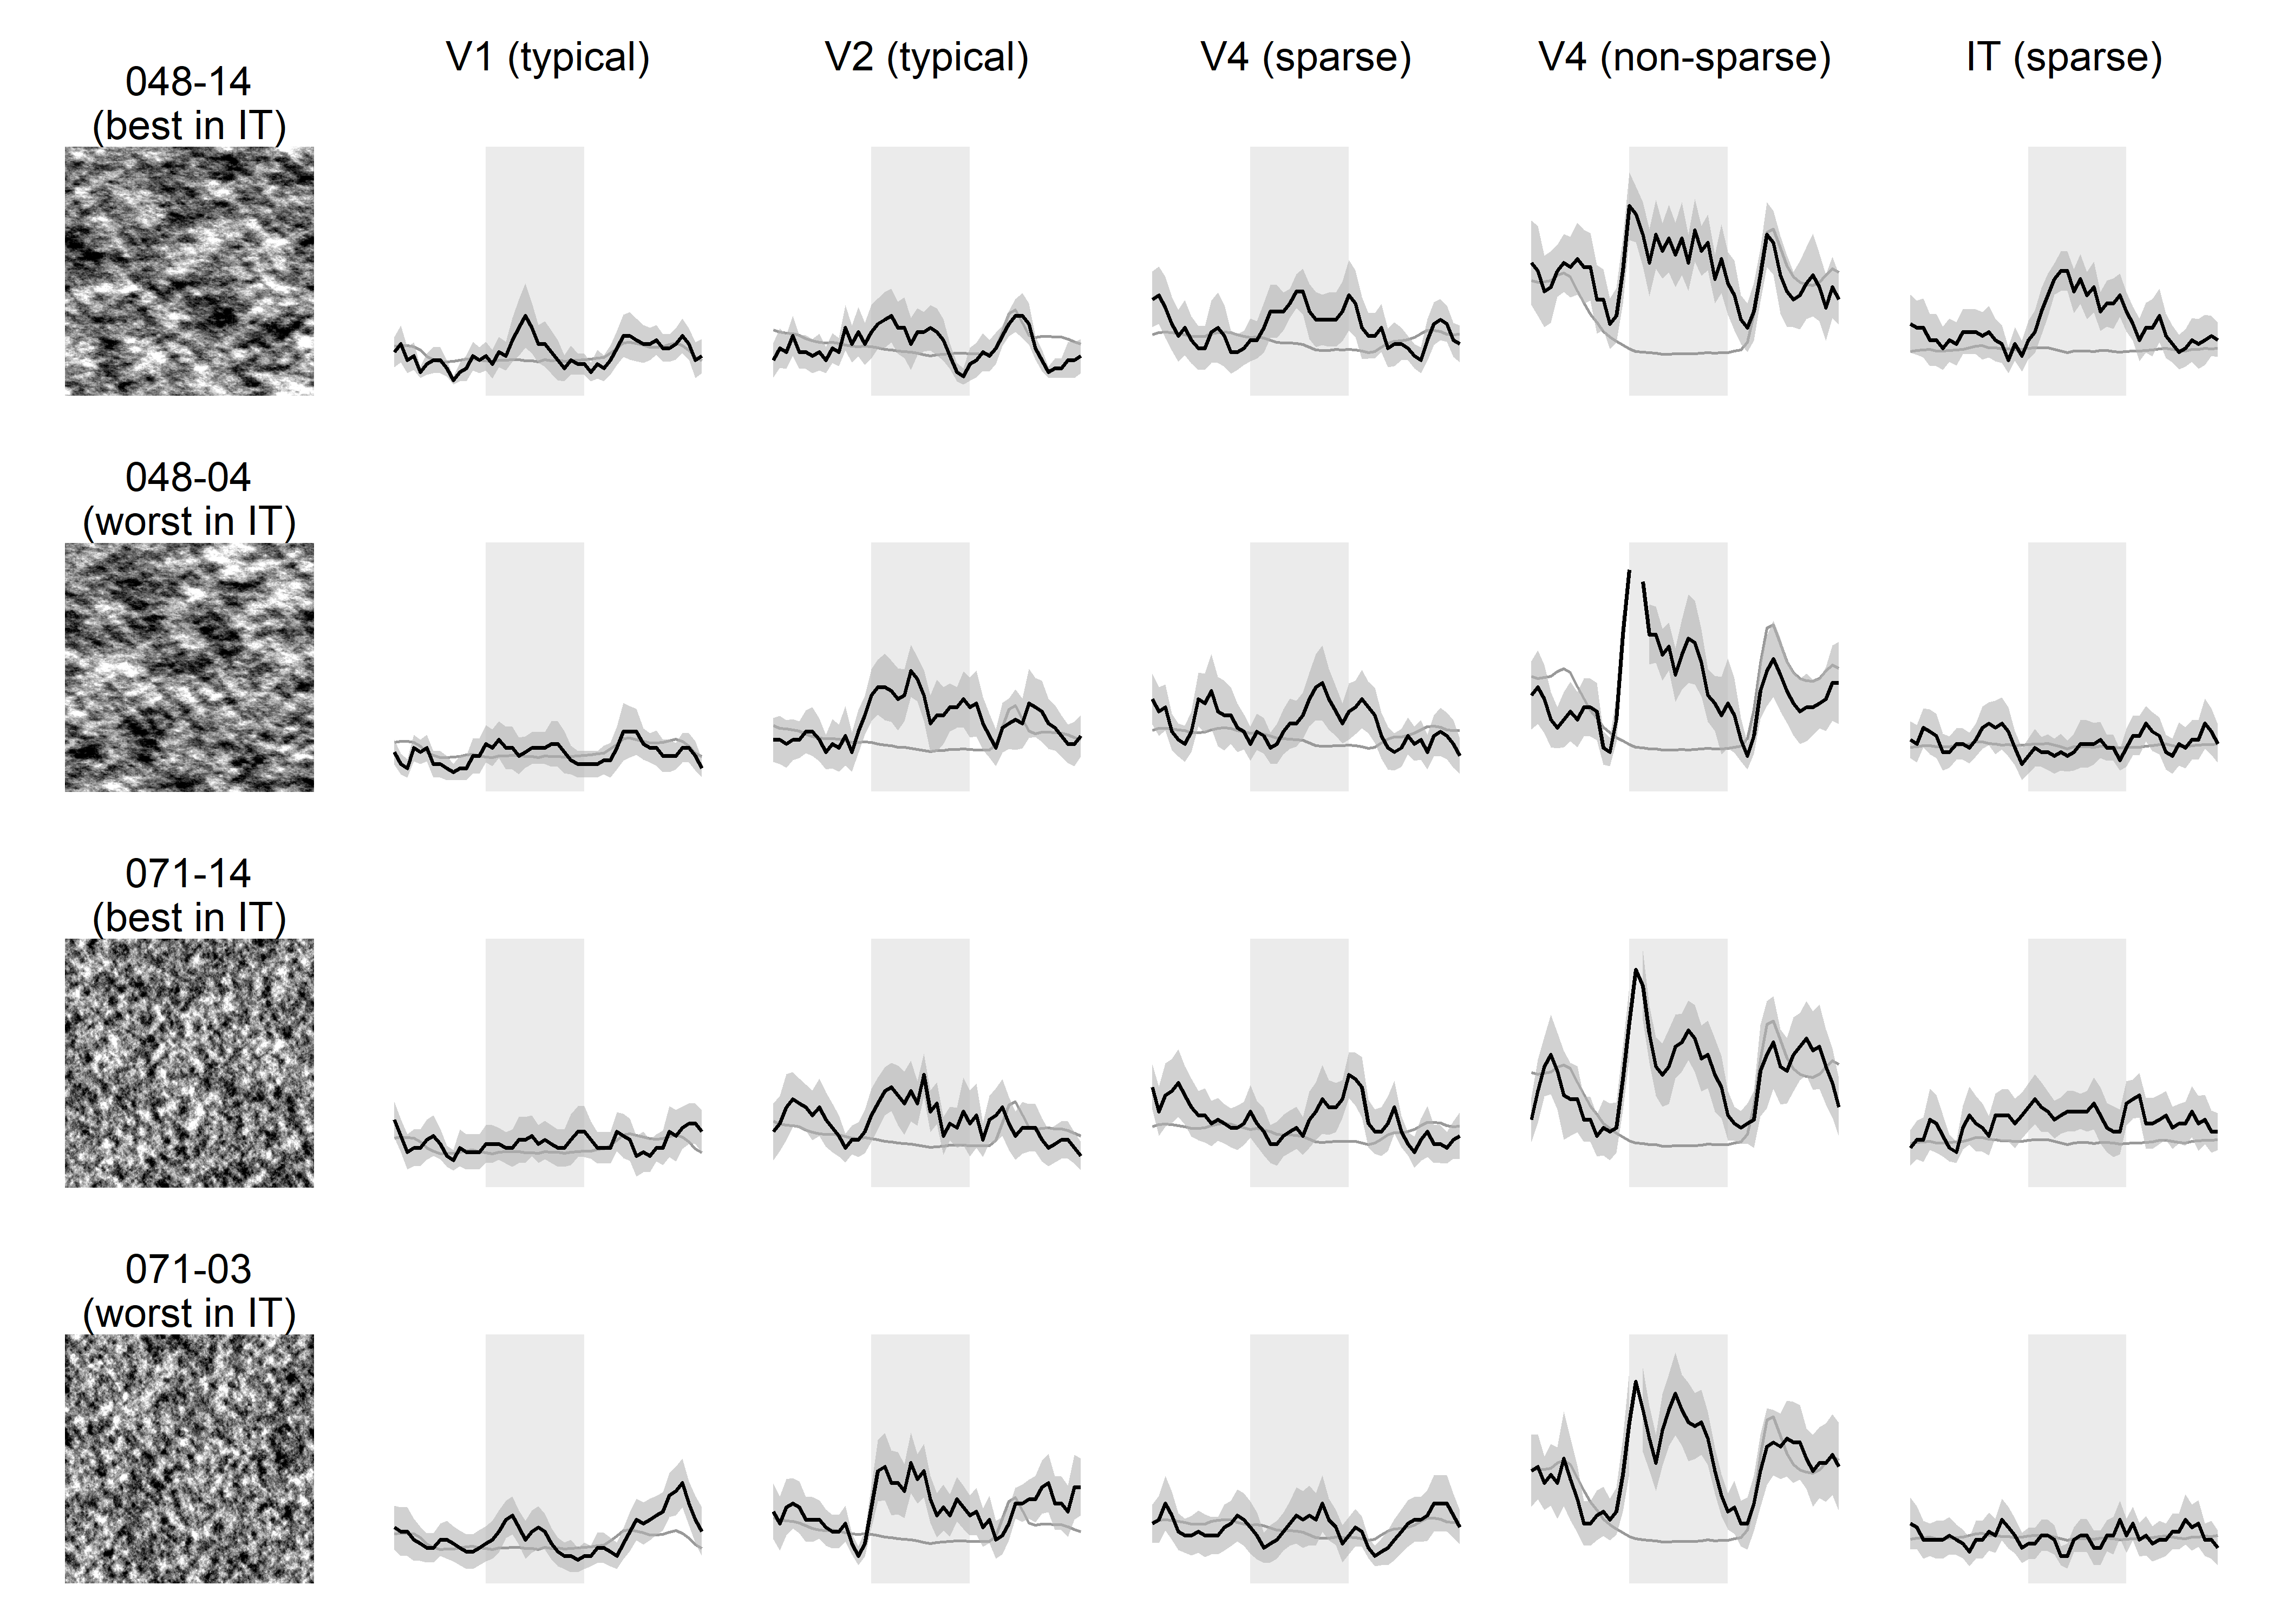
\includegraphics[width=0.8\textwidth]{img/psth_exs.png}
% \end{frame}

% \begin{frame}{Sparsity generally looks to increase along the visual hierarchy}
% \centering
% 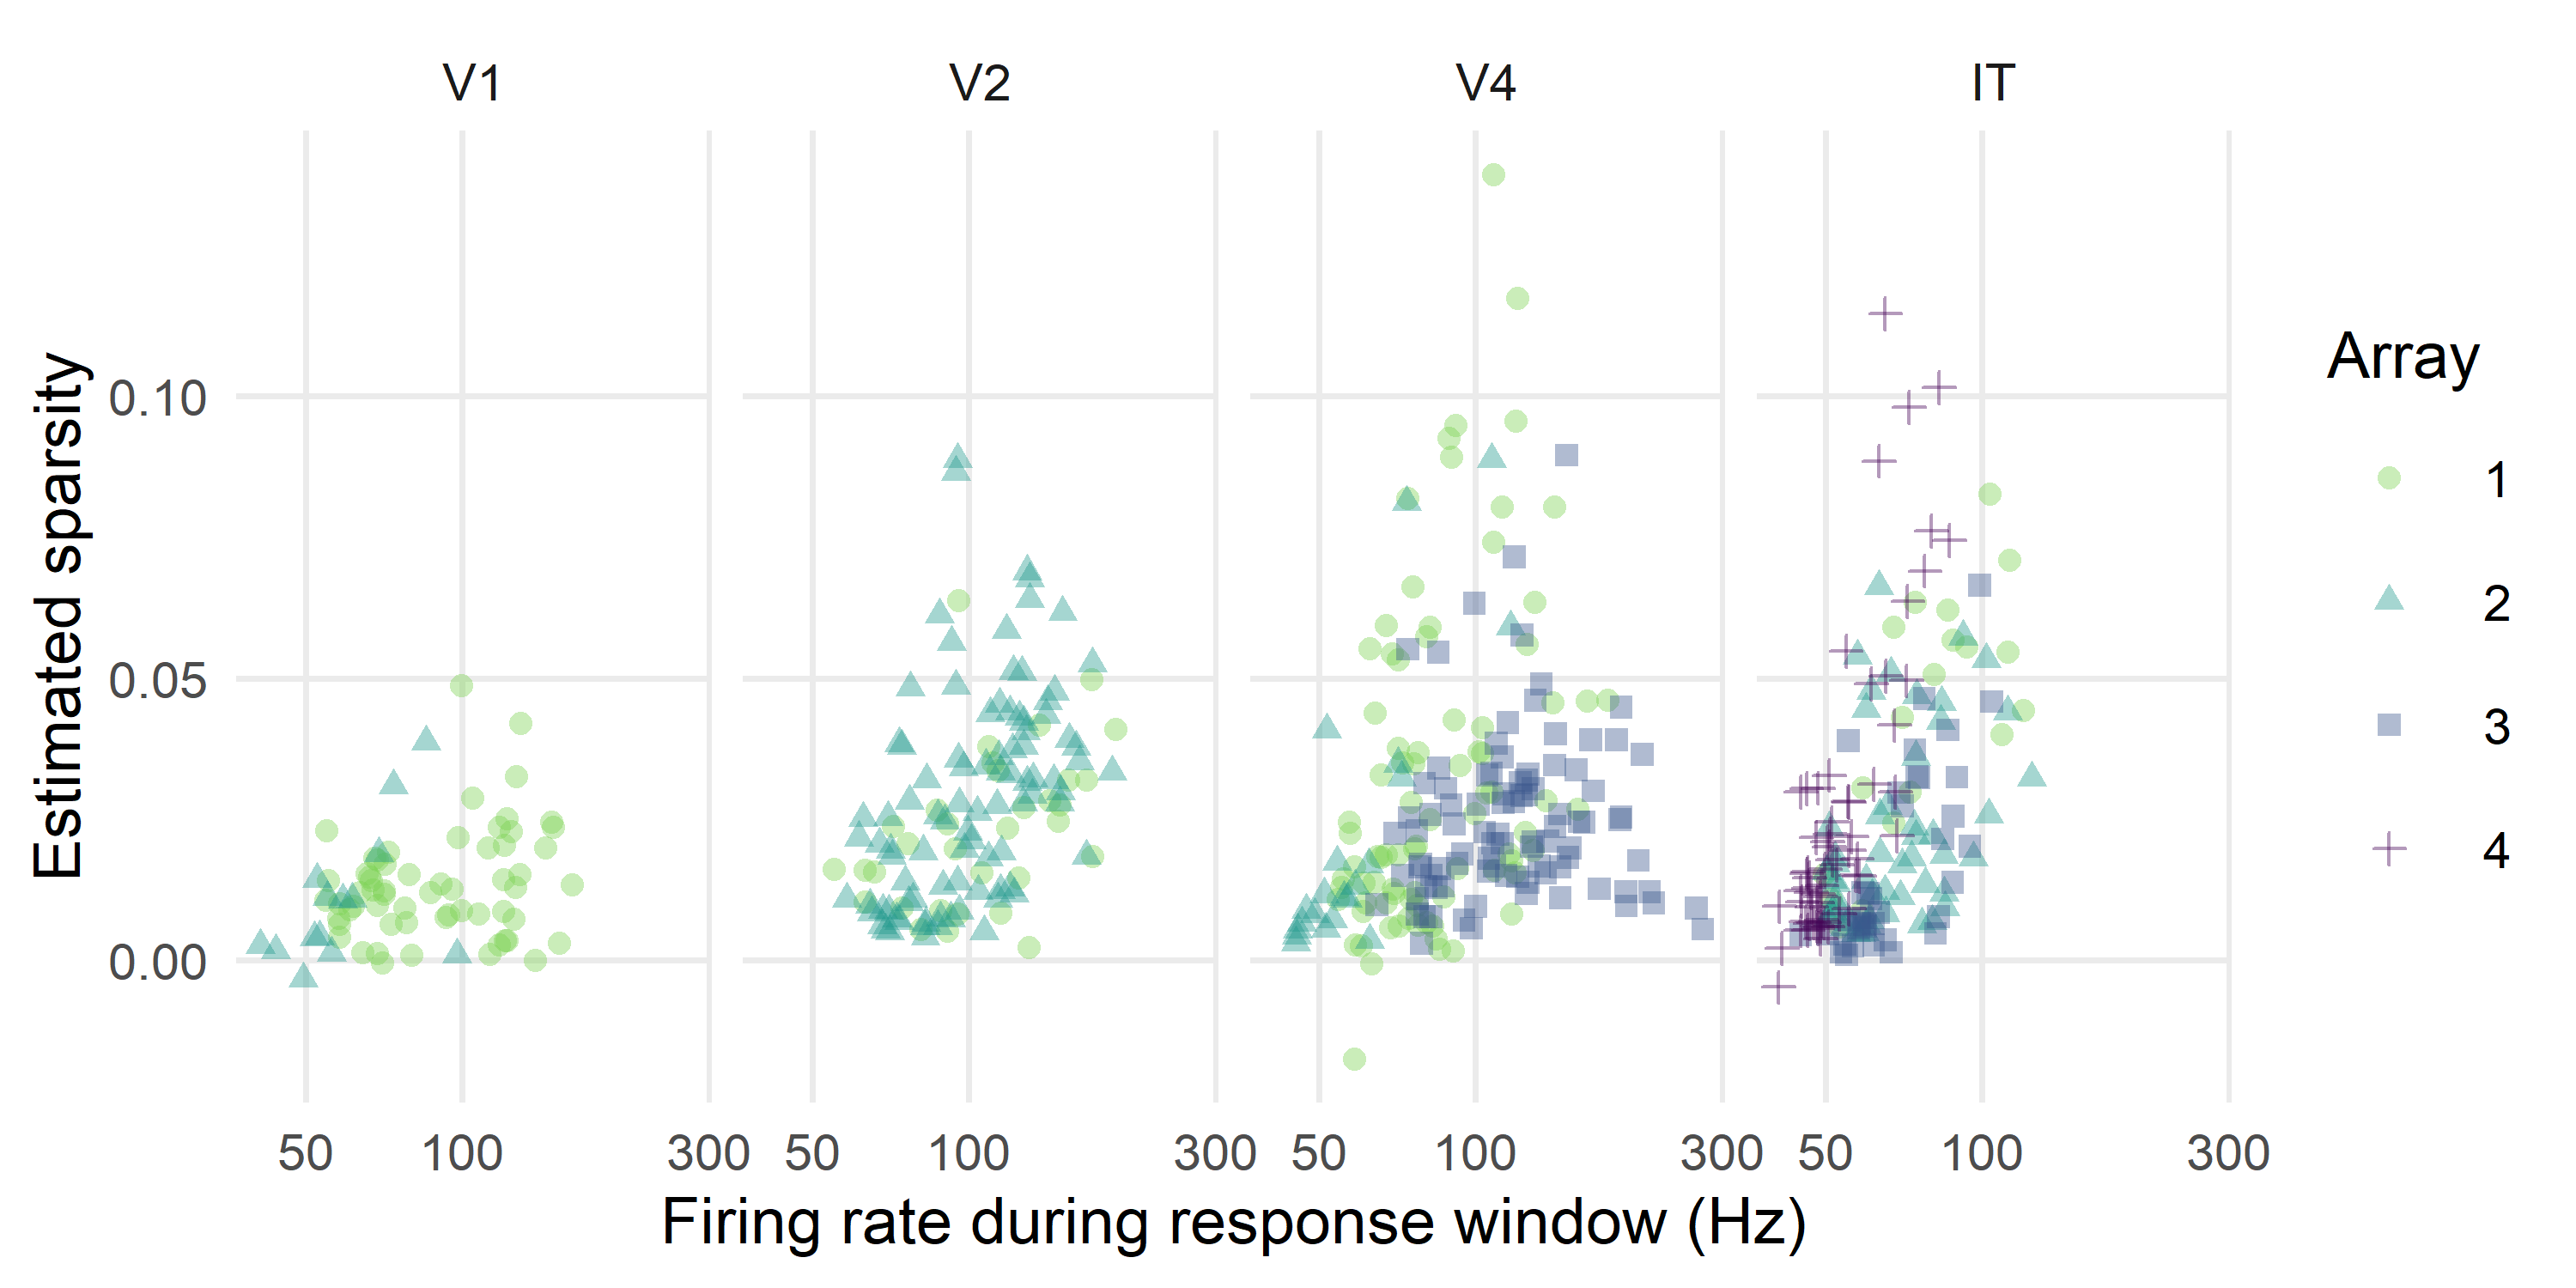
\includegraphics[width=0.8\textwidth]{img/sparsity_vs_rate.png}  
\centering
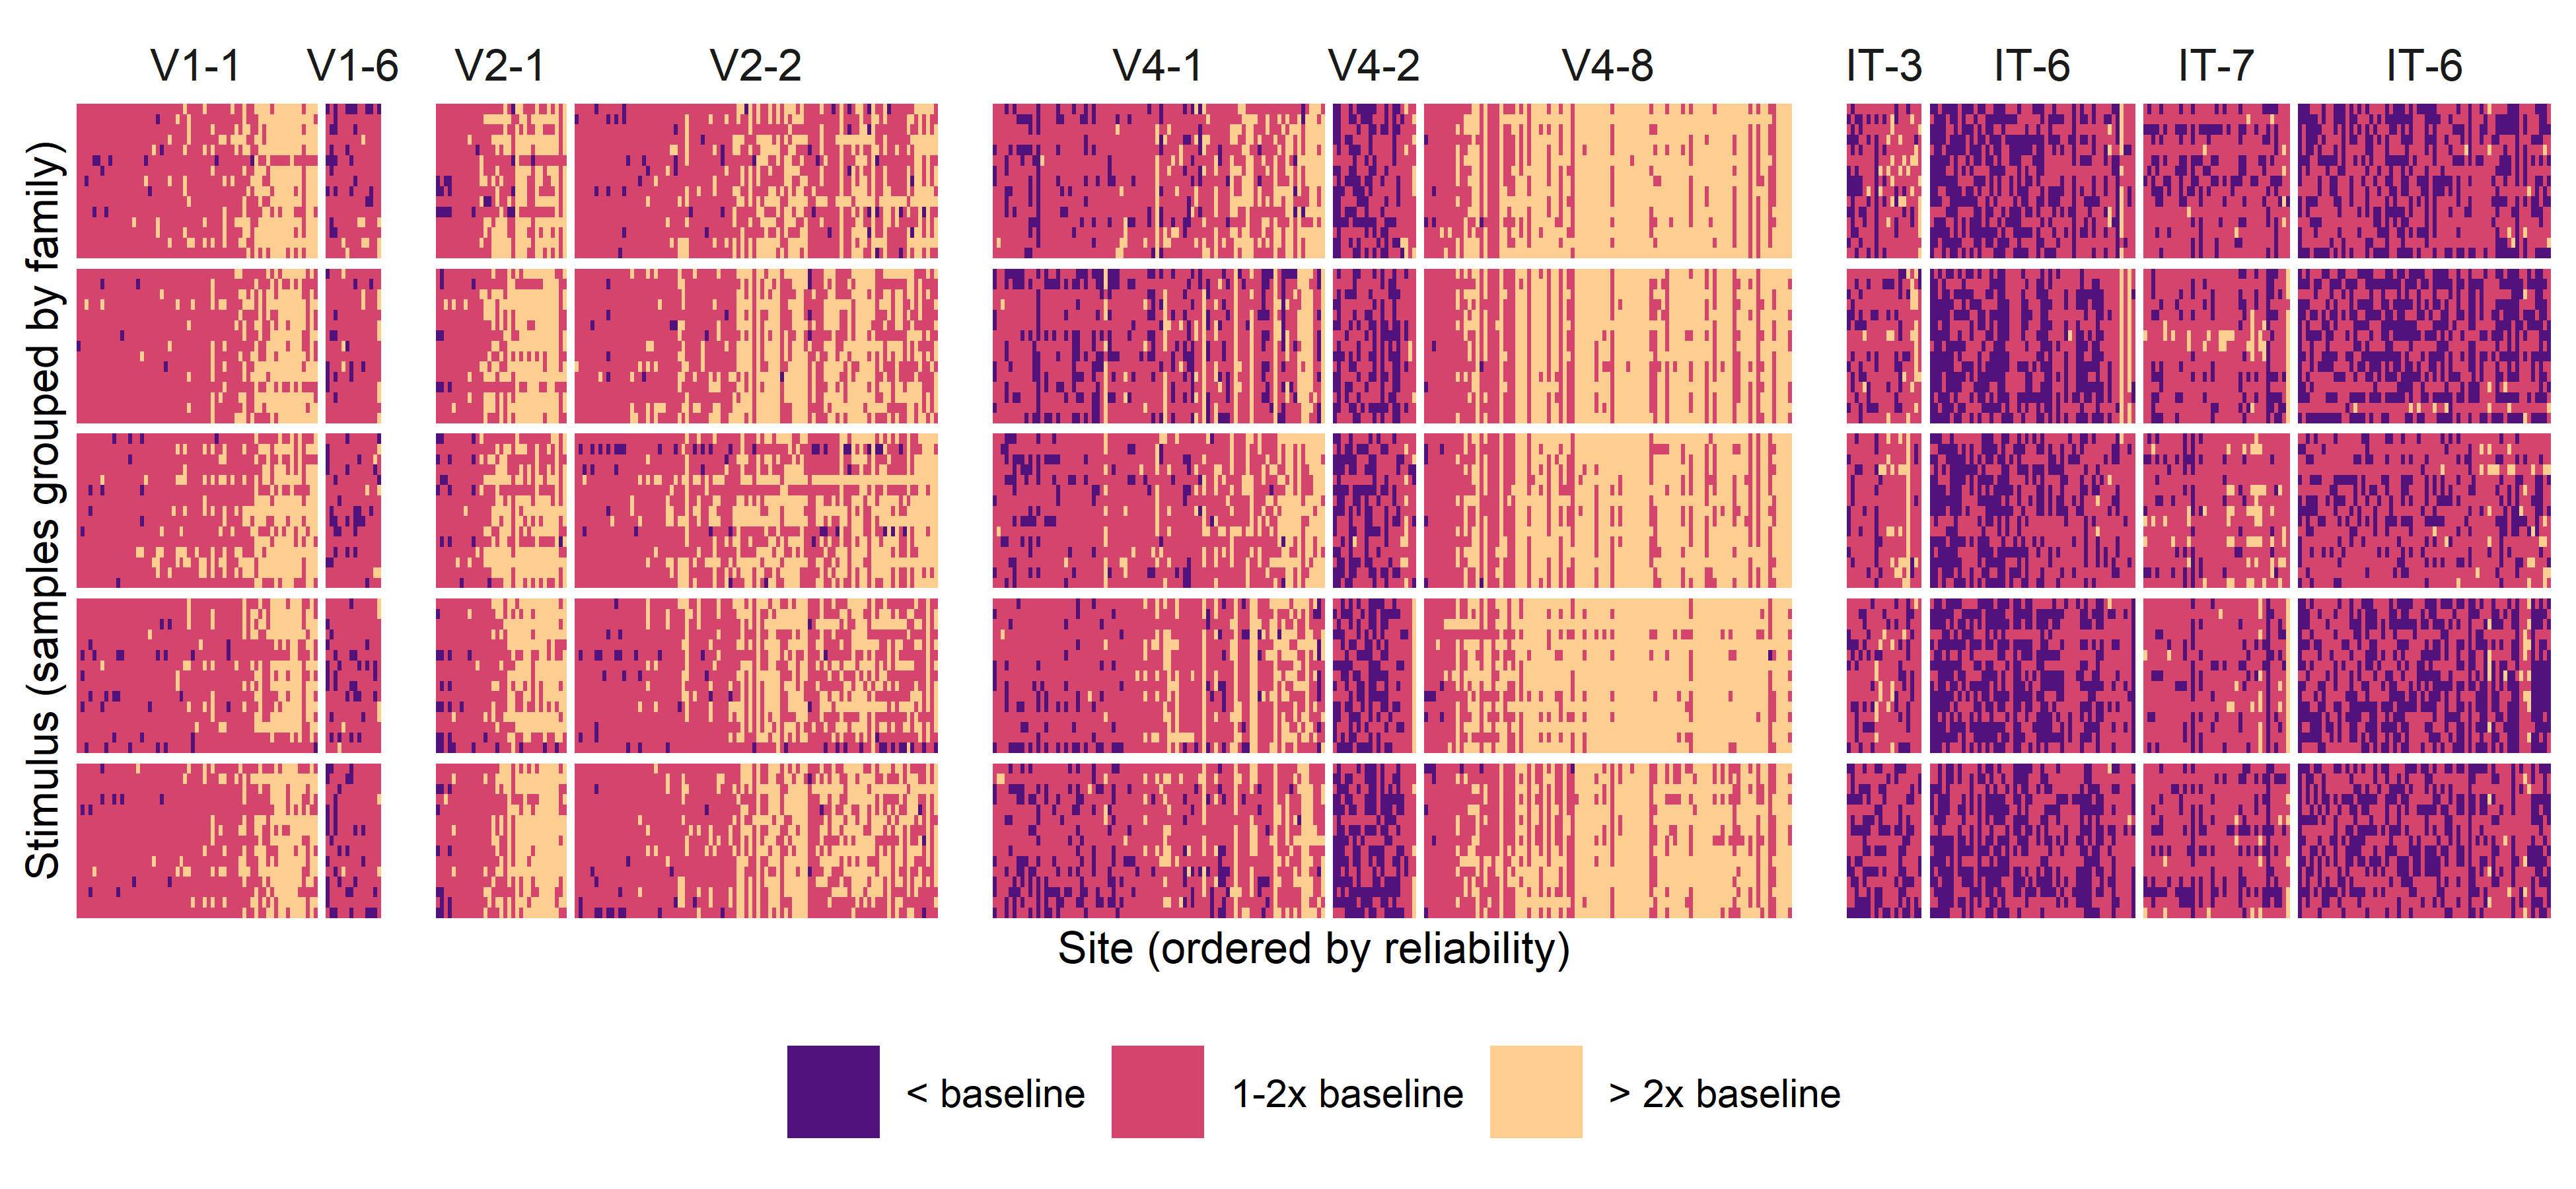
\includegraphics[width=\textwidth]{img/heatmap_arrays_rel02.png}

Sites in IT (columns) tend to show more suppression compared to baseline and less uniformity in the response to stimuli  
% \todo{??: add noise var. estimates?}
\end{frame}

\begin{frame}{Regional differences in reliability and sparsity will affect the analysis strategy}
\begin{align*} 
\mathbf{y}_{f, s(f), r} &= \bfs{\mu} + \mathbf{a}_f + \mathbf{b}_{s(f)} + \mathbf{c}_r + \bfs{\epsilon}_{f, s(f), r}  \\
d_M (\mathbf{a}_{f_1},  \mathbf{a}_{f_2} ) 
&= \sqrt{(\mathbf{a}_{f_1} - \mathbf{a}_{f_2})^\top \bfs{\Sigma}^{-1} (\mathbf{a}_{f_1} - \mathbf{a}_{f_2})} & \textrm{(family-wise)} 
\end{align*}

\begin{itemize}
    \item Reliability: ratio of signal variance / noise variance \pause
    \item Sparsity: distribution of a site's response to the stimulus \pause 
    \item Intuition: these features correspond to the two components of Mahalanobis distance (difference-in-means, precision)
\end{itemize}
\end{frame}


% \begin{frame}{Model of texture family separation in neural responses}
% \begin{align*}
% \mathbf{y}_{f, s(f), r} &= \bfs{\mu} + \mathbf{a}_f + \mathbf{b}_{s(f)} + \mathbf{c}_r + \bfs{\epsilon}_{f, s(f), r} 
% \end{align*}
% \begin{itemize}
%     \item \( d_M: \mathbb{R}^p \times \mathbb{R}^p \to \mathbb{R} \): Mahalanobis distance
% \end{itemize}
% \begin{align*} 
% & d_M (\mathbf{a}_{f_1},  \mathbf{a}_{f_2} )  &  \textrm{(family-wise)} \\
% & d_M (\mathbf{b}_{s_1 (f)}, \mathbf{b}_{s_2 (f)}) & \textrm{(sample-wise)} 
% \end{align*}
% \end{frame}


% \begin{frame}{We estimated reliability as Brown-Spearman corrected split-half correlation}
% \begin{enumerate}
%     \item Split observations based on the repetitions into two groups of three \pause 
%     \item Average observations in each split over the repetitions \pause 
%     \item Calculate the correlation between the splits and apply Fisher's \( z \)-transform \pause 
%     \item Average the calculated \( z \)-transformed split-half correlations over all \( \binom{6}{3} / 2 = 10 \) possible repetition splits \pause 
%     \item Apply the Brown-Spearman correction
% \end{enumerate}
% \end{frame}

\begin{frame}{Reliability of sites is region- and array-specific}
\centering
Reliability can be found with split-half correlation. 

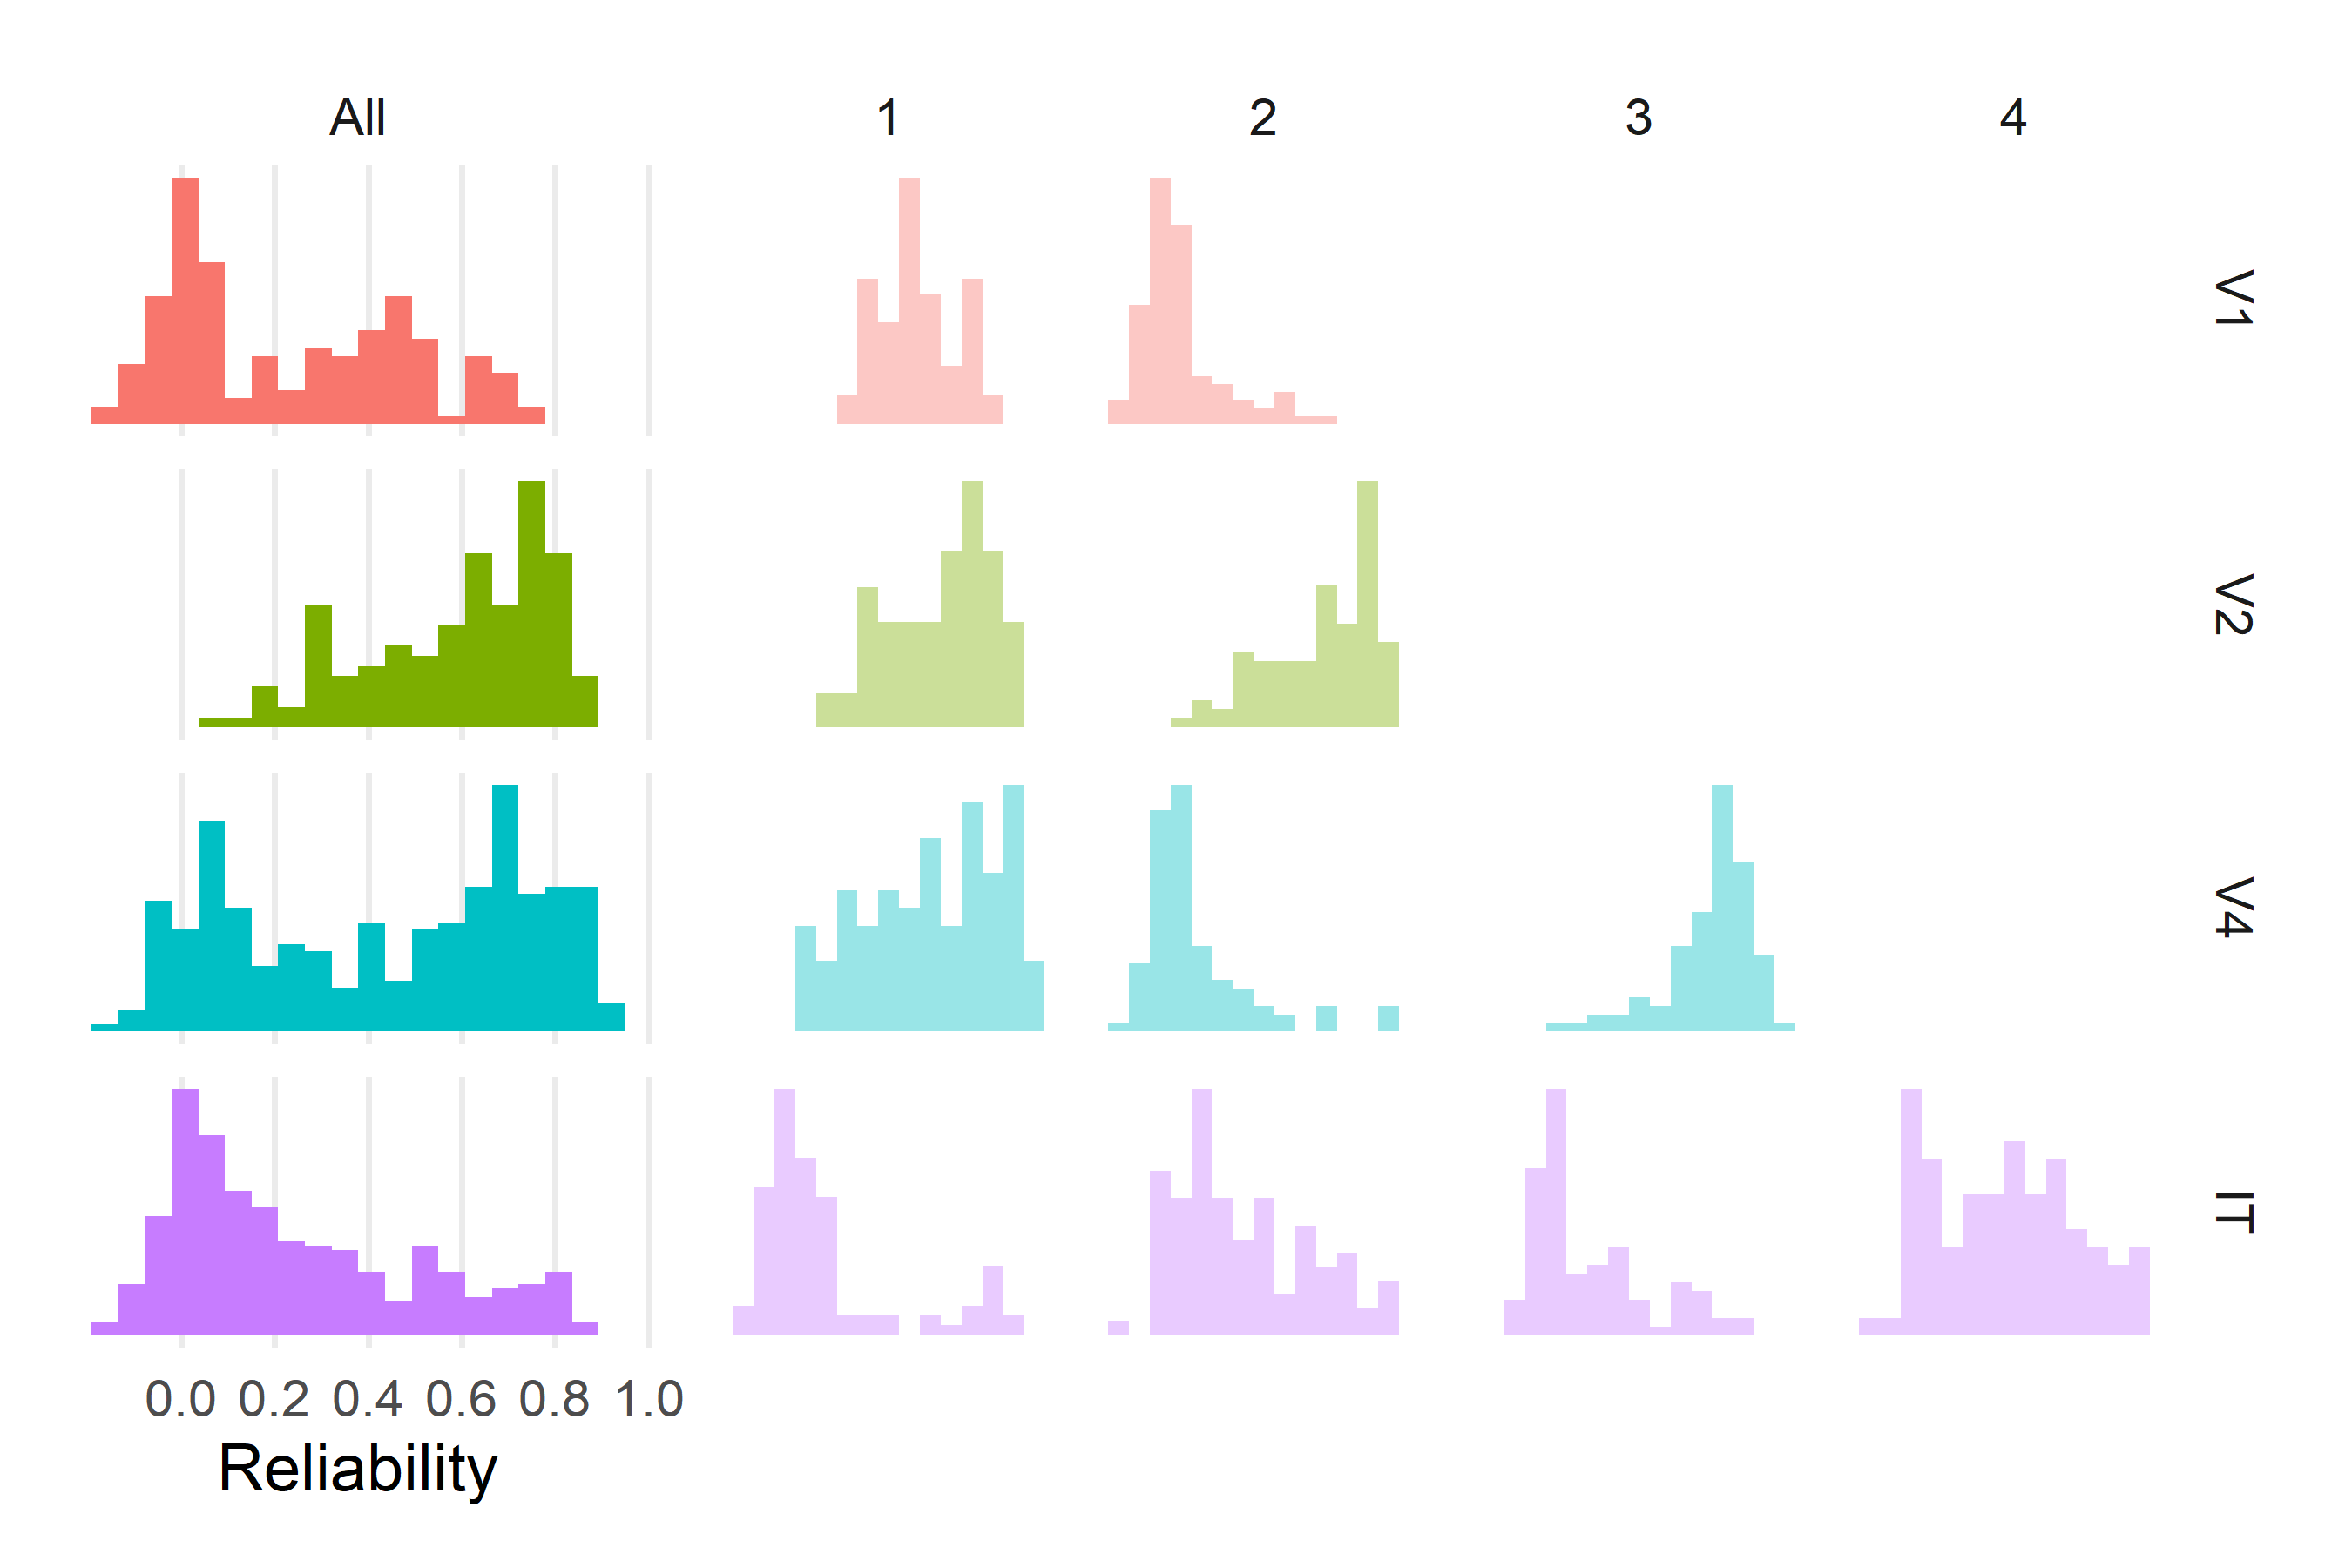
\includegraphics[width=0.8\textwidth]{img/region_array_reliability.png} 

\end{frame}

\begin{frame}{Lifetime sparsity characterizes a single site's response distribution to the stimuli}

\begin{itemize}
    \item We examined the \hl{lifetime sparseness} of each recording site \parencite{willmore_characterizing_2001}. \pause 
    \item  High sparseness indicates a heavy-tailed response distribution to stimuli \pause 
    \item \parencite{rolls_sparseness_1995, vinje_sparse_2000} A common sparseness measure in neuroscience is Treves-Rolls, based on a ratio of moments \pause 
    \item \( S_{\textrm{TR}} = \left( 1 - \frac{\left( \frac{1}{n} \sum_{i = 1}^n \mu_{i} \right)^2}{\frac{1}{n} \sum_{i = 1}^n \mu_{i}^2} \right) \left( \frac{1}{1 - \frac{1}{n}} \right) \) 
\end{itemize}
\end{frame}

\begin{frame}{Many approaches to measure sparsity reduce to a ratio of moments}

\begin{itemize}
    \item \parencite{hurley_comparing_2009} Other common sparsity measures reduce to a normalization of \( L_2 / L_1 \) (e.g., Hoyer) \pause 
    \item Exceptions: kurtosis, Gini index \pause 
    \item Empirical differences small on our non-extreme data
\end{itemize}

\begin{center}
    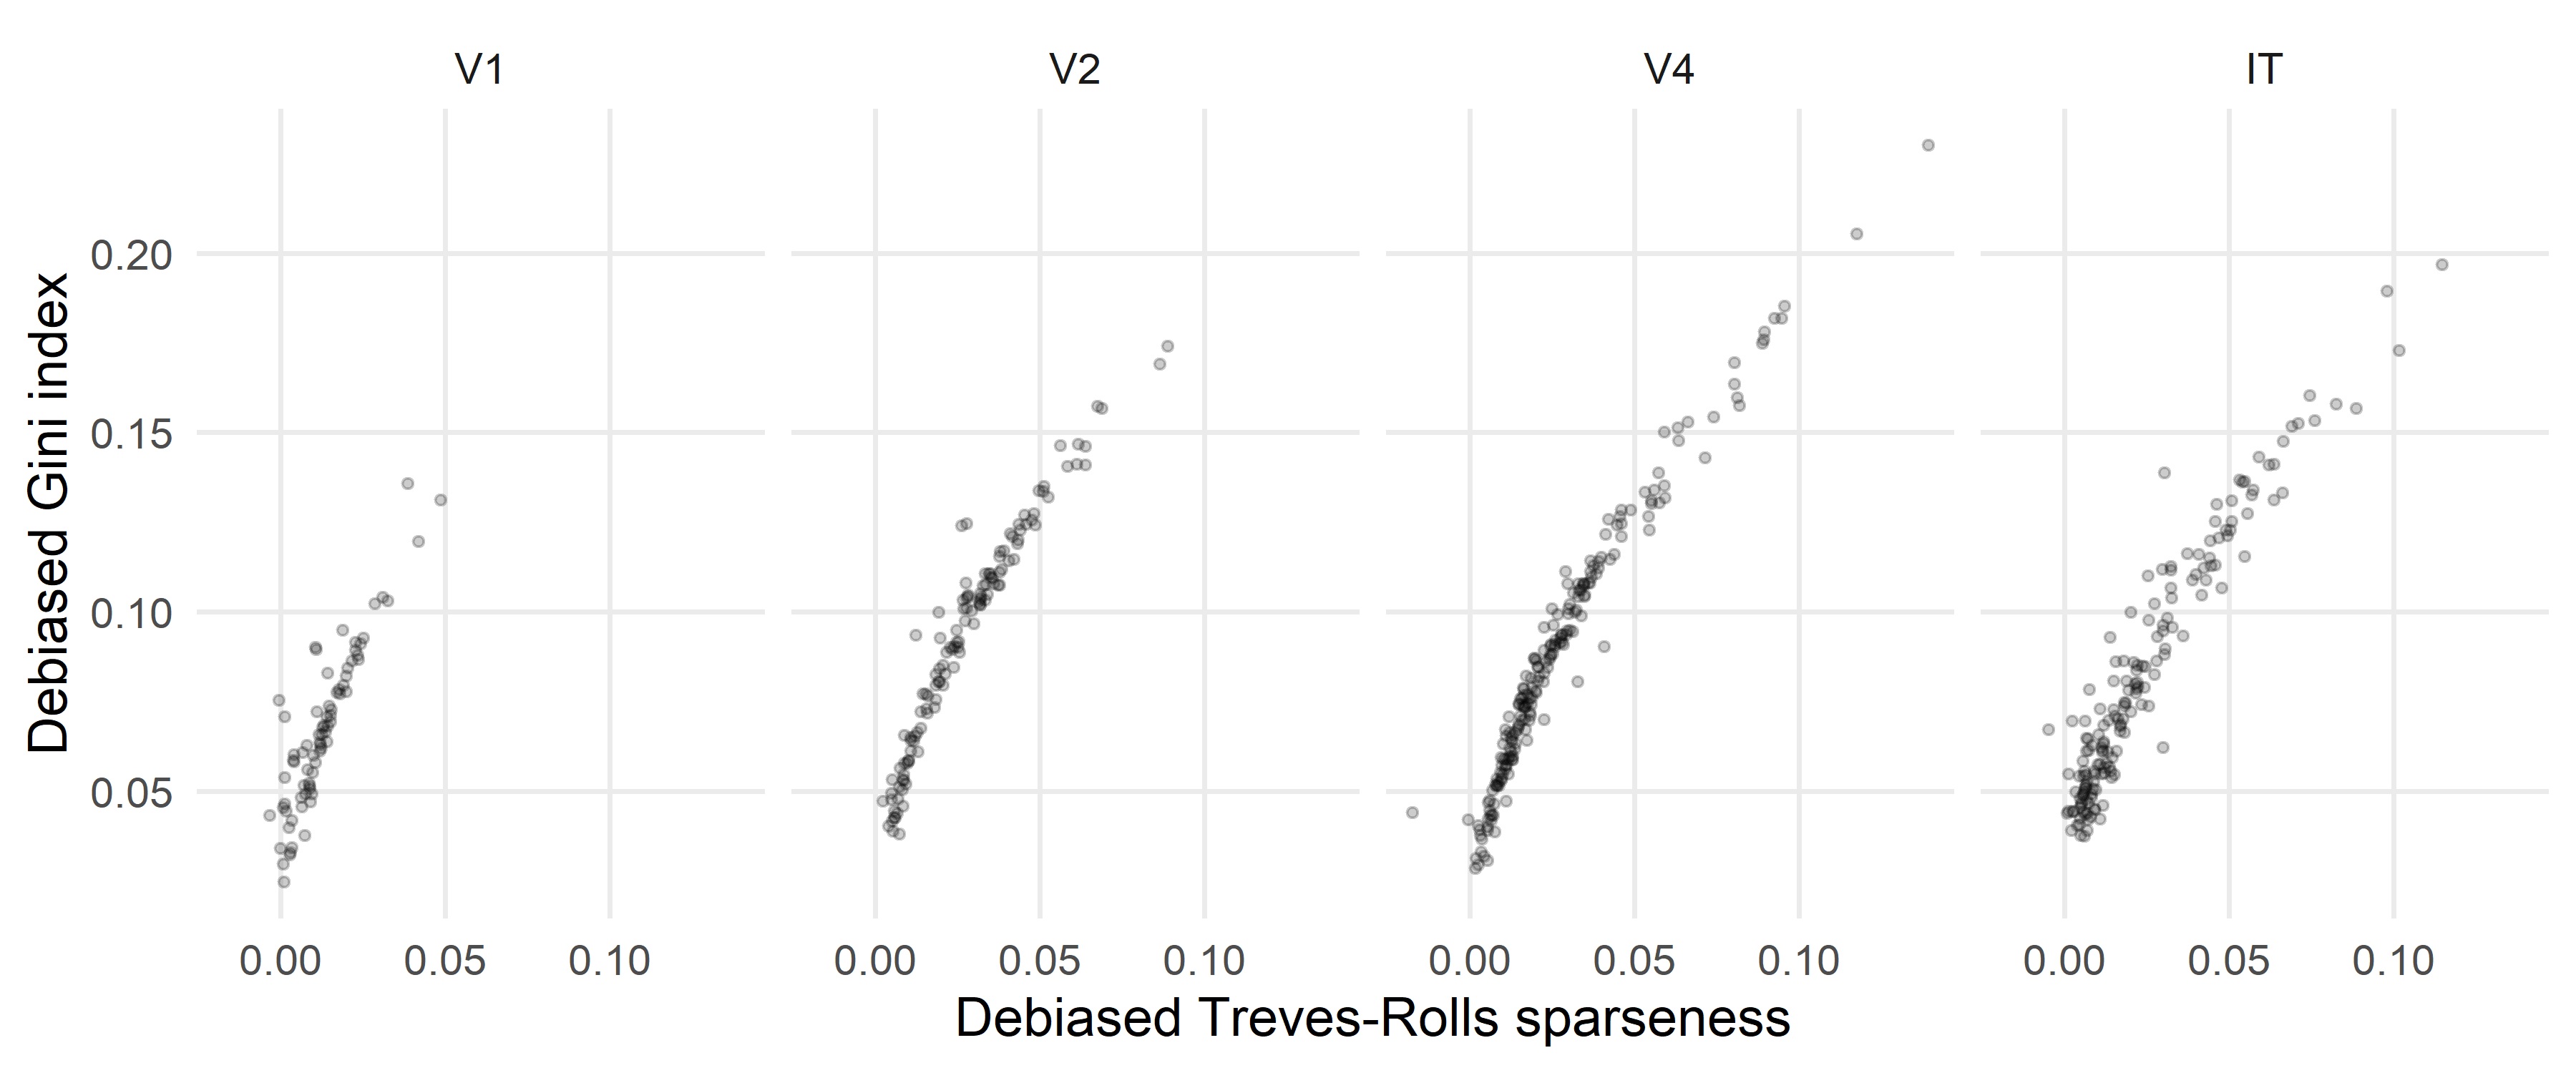
\includegraphics[width=0.8\textwidth]{img/gini_tr.png}
\end{center}
\end{frame}

\begin{frame}{Sparsity between regions is fairly similar}
\begin{itemize}
    \item For most sparsity estimators, noise variance produces an upwards bias \parencite{pospisil_unbiased_2021} \pause 
    % \item \todo{??: include derivation in slide?}
    \item Bias produces the strongest effect in IT.
\end{itemize}

\begin{center}
    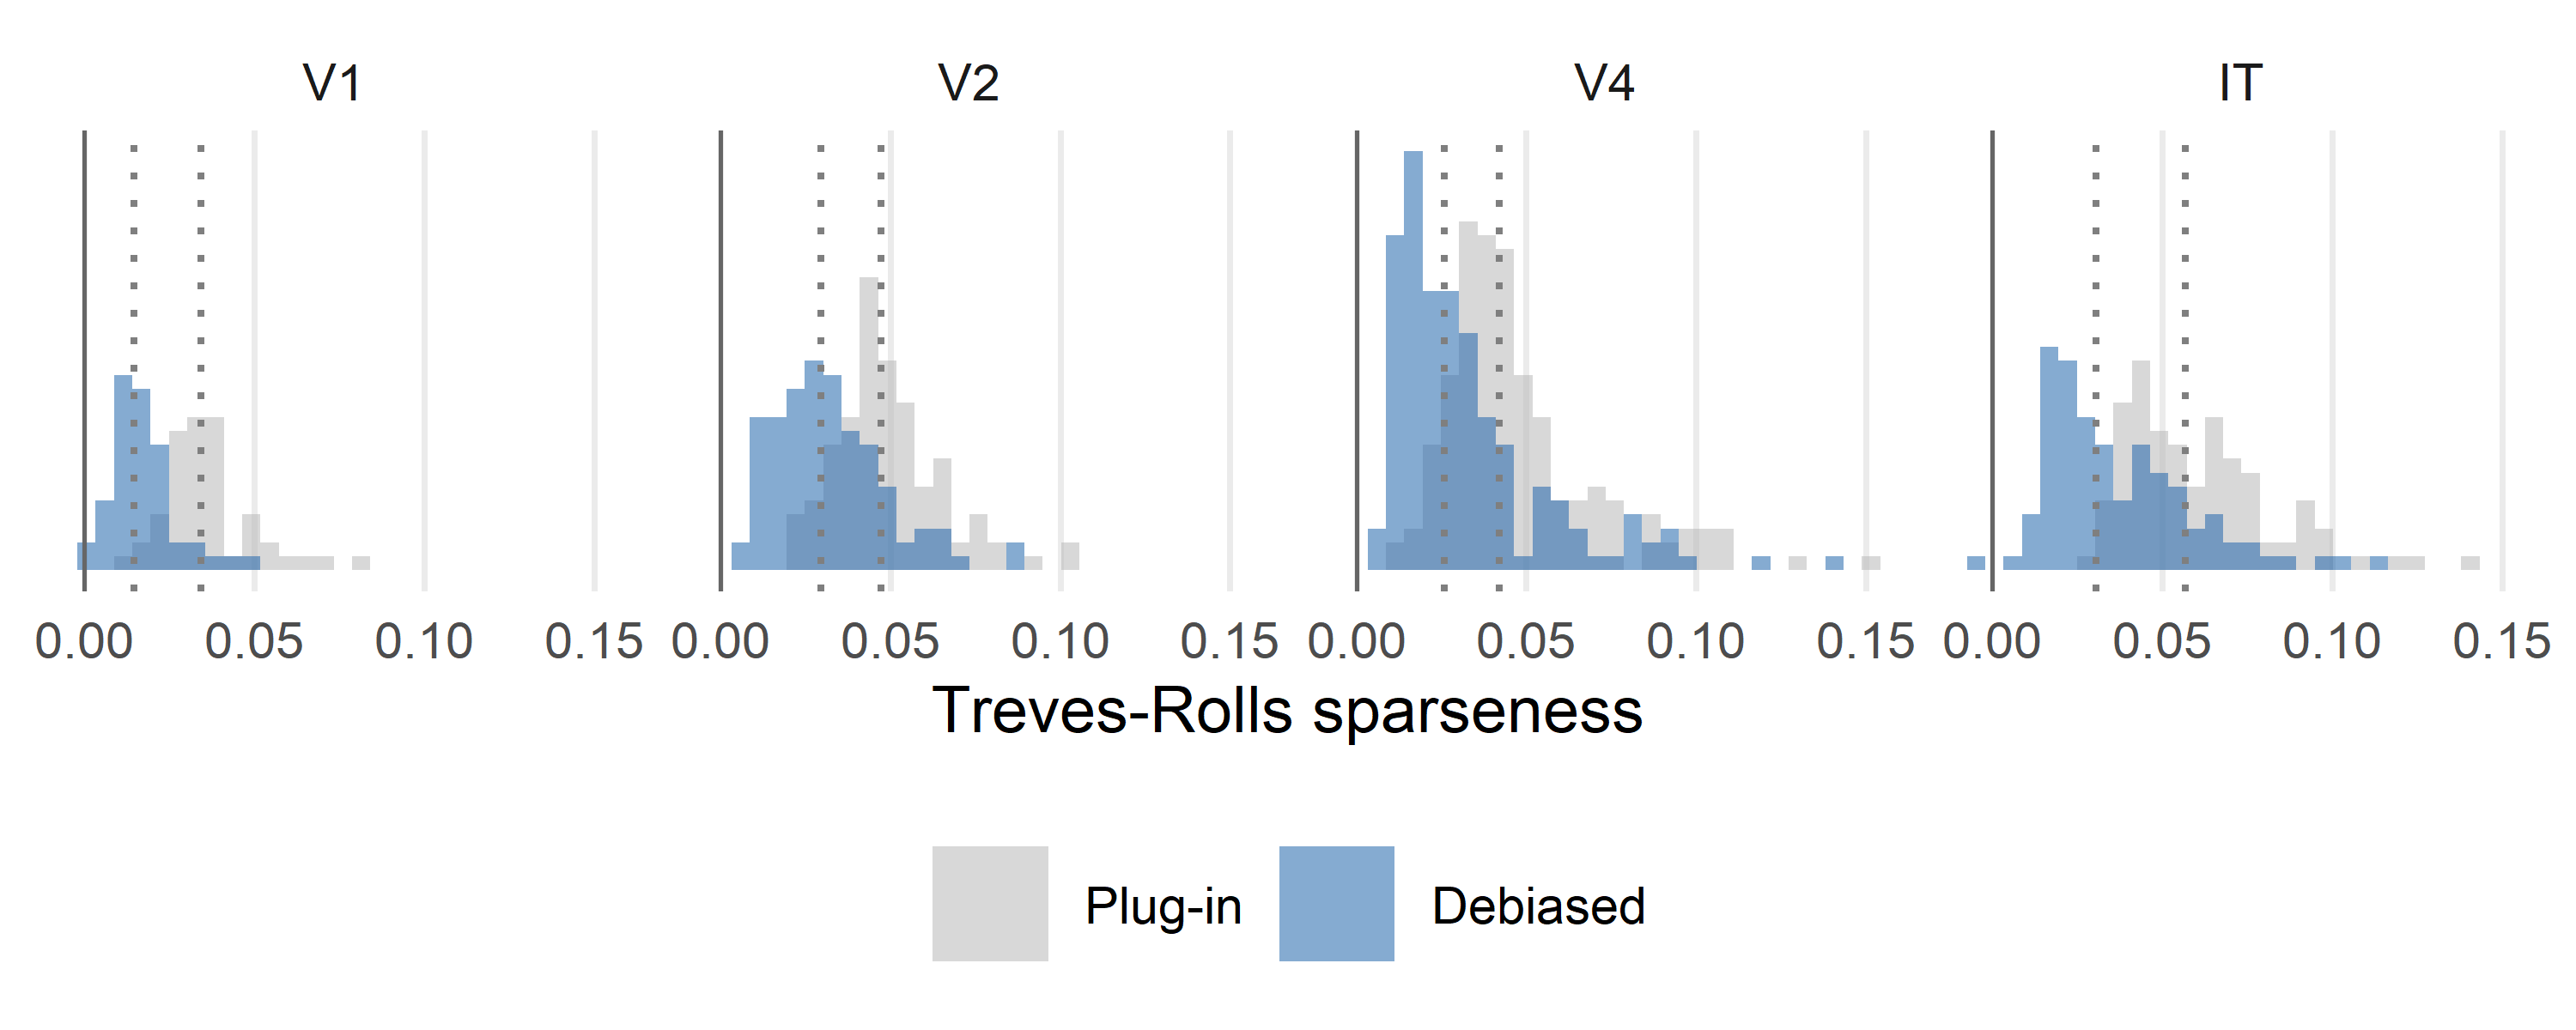
\includegraphics[width=0.9\textwidth]{img/tr_hist-rel04.png}

    (filtered for reliability \( > 0.4 \)).
\end{center}
\end{frame}

% \begin{frame}{Sparsity and reliability are related, with regional differences related to location on a curve}
% \todo{TODO: write up the definitional derivation of these curves.}
% \todo{TODO: if the point is that IT has more sparsity, choose a different visualization.}

% \centering
% 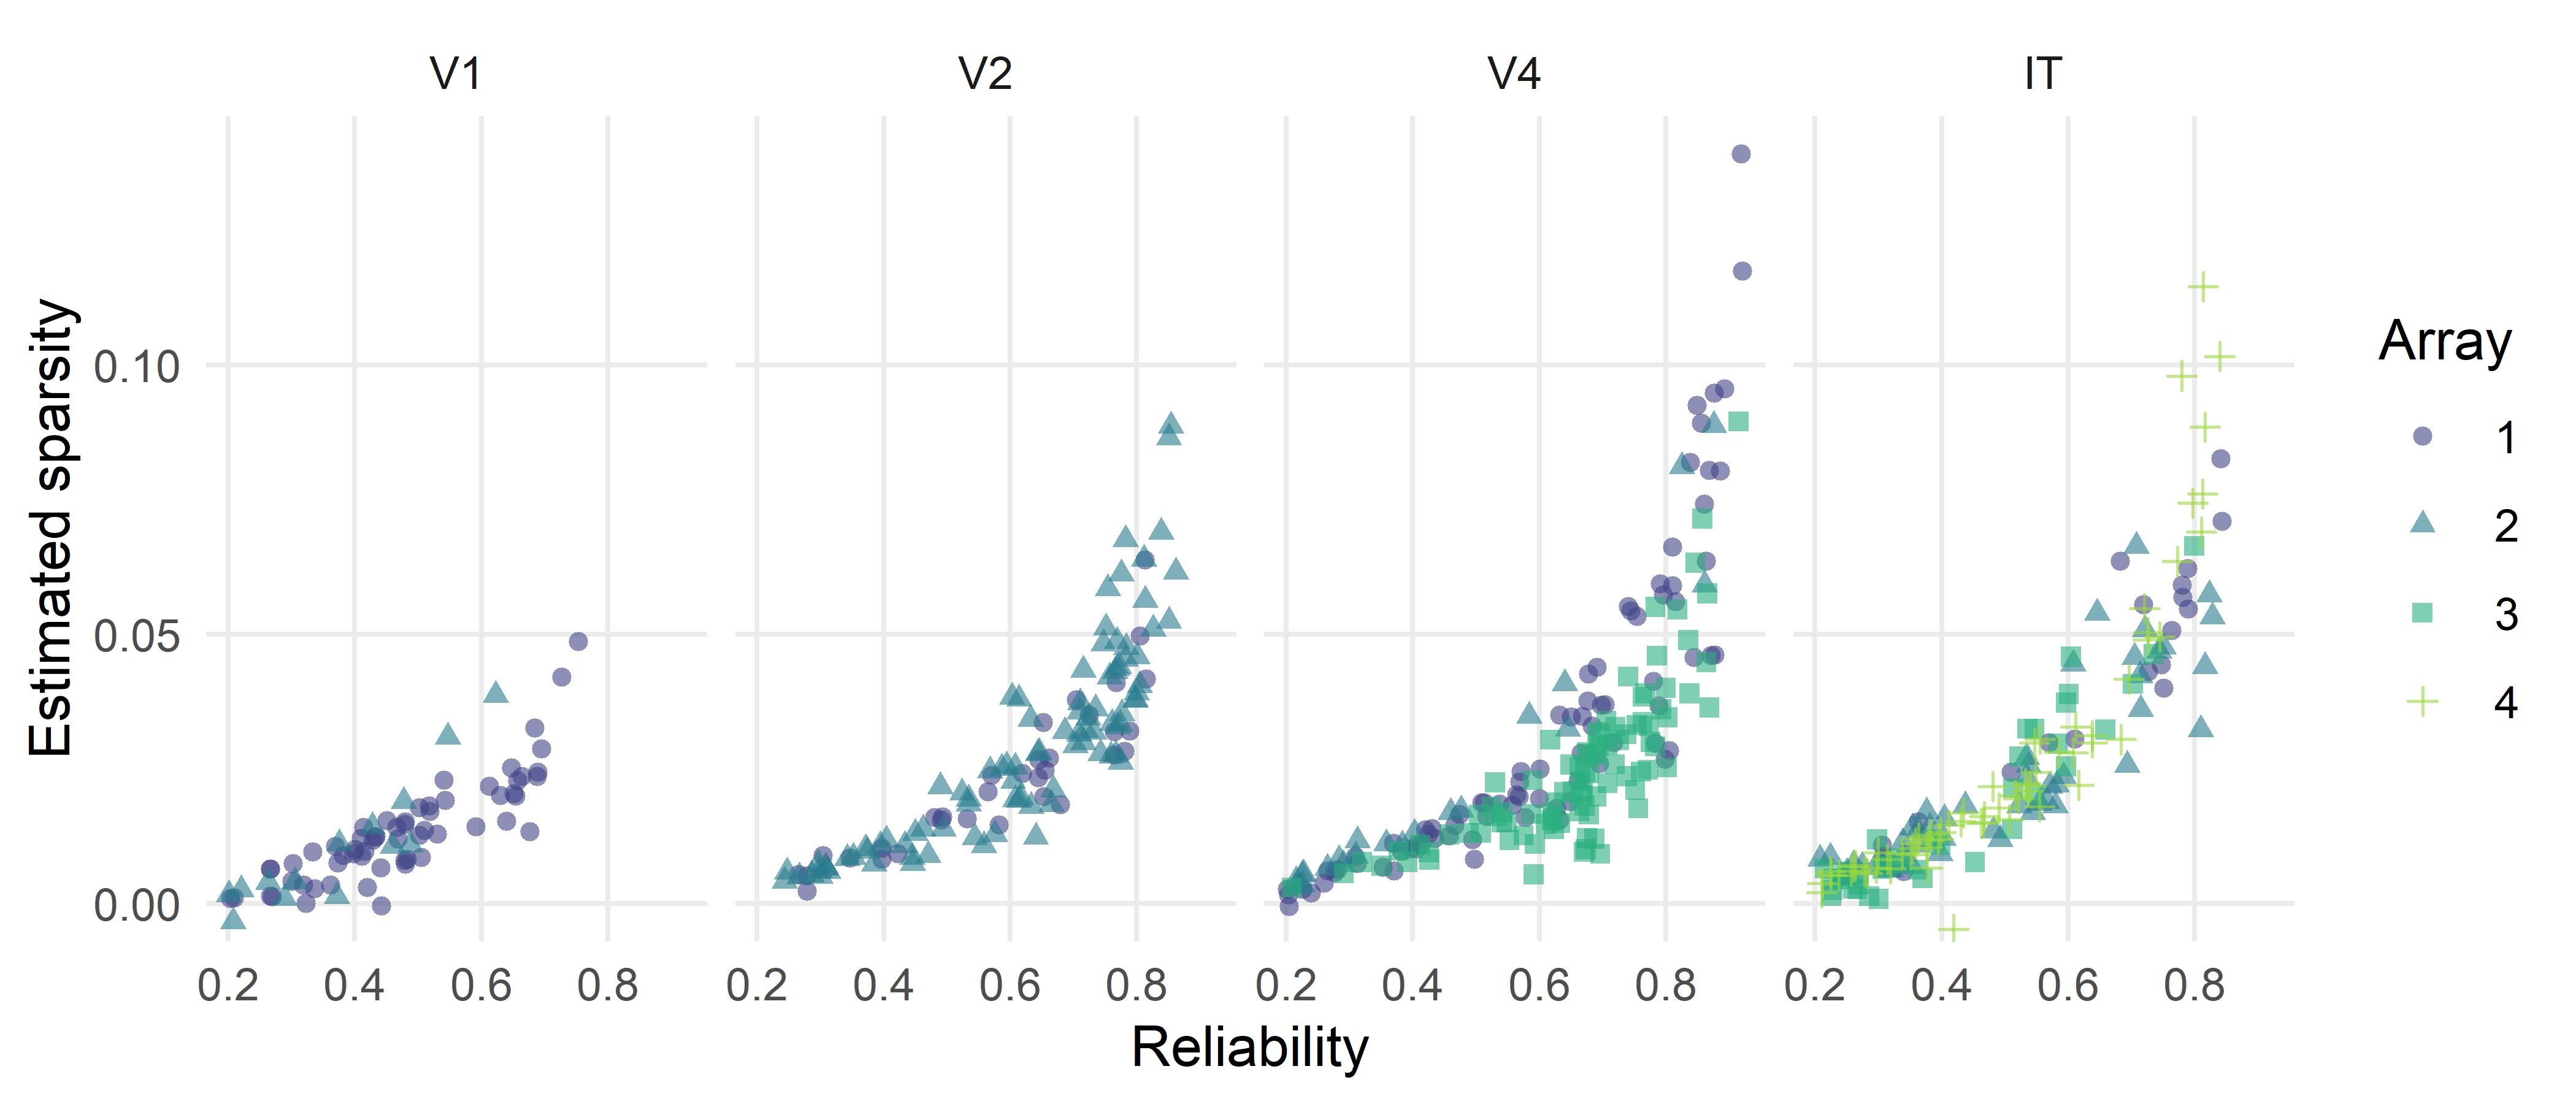
\includegraphics[width=\textwidth]{img/sparsity_reliability_array.png}
% \end{frame}

\section{Results}

\begin{frame}{Approach}
    \begin{enumerate}
        {\color{gray} \item Define a model of neural separability}
        {\color{gray} \item  Identify inter-region differences that affect separability estimation }
        \item  Correct for regional differences to produce comparable separability estimates
    \end{enumerate}
\end{frame}

\begin{frame}{Two approaches to correcting for reliability}
\begin{columns}
\begin{column}{0.5\textwidth}
\textbf{Sub-sampling}
    \begin{enumerate}
        \item Select some range of reliability, e.g., \( \rho \in [0.5, 0.7] \) \pause 
        % \item Remove sites whose estimated reliabilities fall outside of the range \pause
        \item Sample \( p \) sites from each region \pause 
        \item Find \( \hat{D} \) for all \( \binom{35}{2} \) pairwise family comparisons \pause
        \item Report the mean \pause
        \item Repeat (2-4) 200 times \pause 
        \item Repeat (1-5) for other reliability ranges \pause 
    \end{enumerate}
\end{column}
\begin{column}{0.5\textwidth}
\textbf{Stratification}
    \begin{enumerate}
        \item Set some bins of reliability, e.g., \( \{ [0.3, 0.4], [0.4, 0.5], \dots, [0.7, 0.8]\} \) \pause 
        \item For each region, take 3 sites from each bin (e.g., if there are 5 bins, \( p = 15 \)) \pause
        \item ... 
        % \item Find \( \hat{D} \) for all pairwise family comparisons
        % \item Report the mean of the pairwise family comparisons 
        % \item Repeat the sampling 200 times \pause
    \end{enumerate}
\end{column}
\end{columns}
\end{frame}

\begin{frame}{Reliability influences the calculated between-family distance, but inter-region rankings remain consistent}

Resampling with \( p = 15 \) and 200 repetitions. 

\vspace{10pt}

\begin{columns}
\begin{column}{0.57\textwidth}
    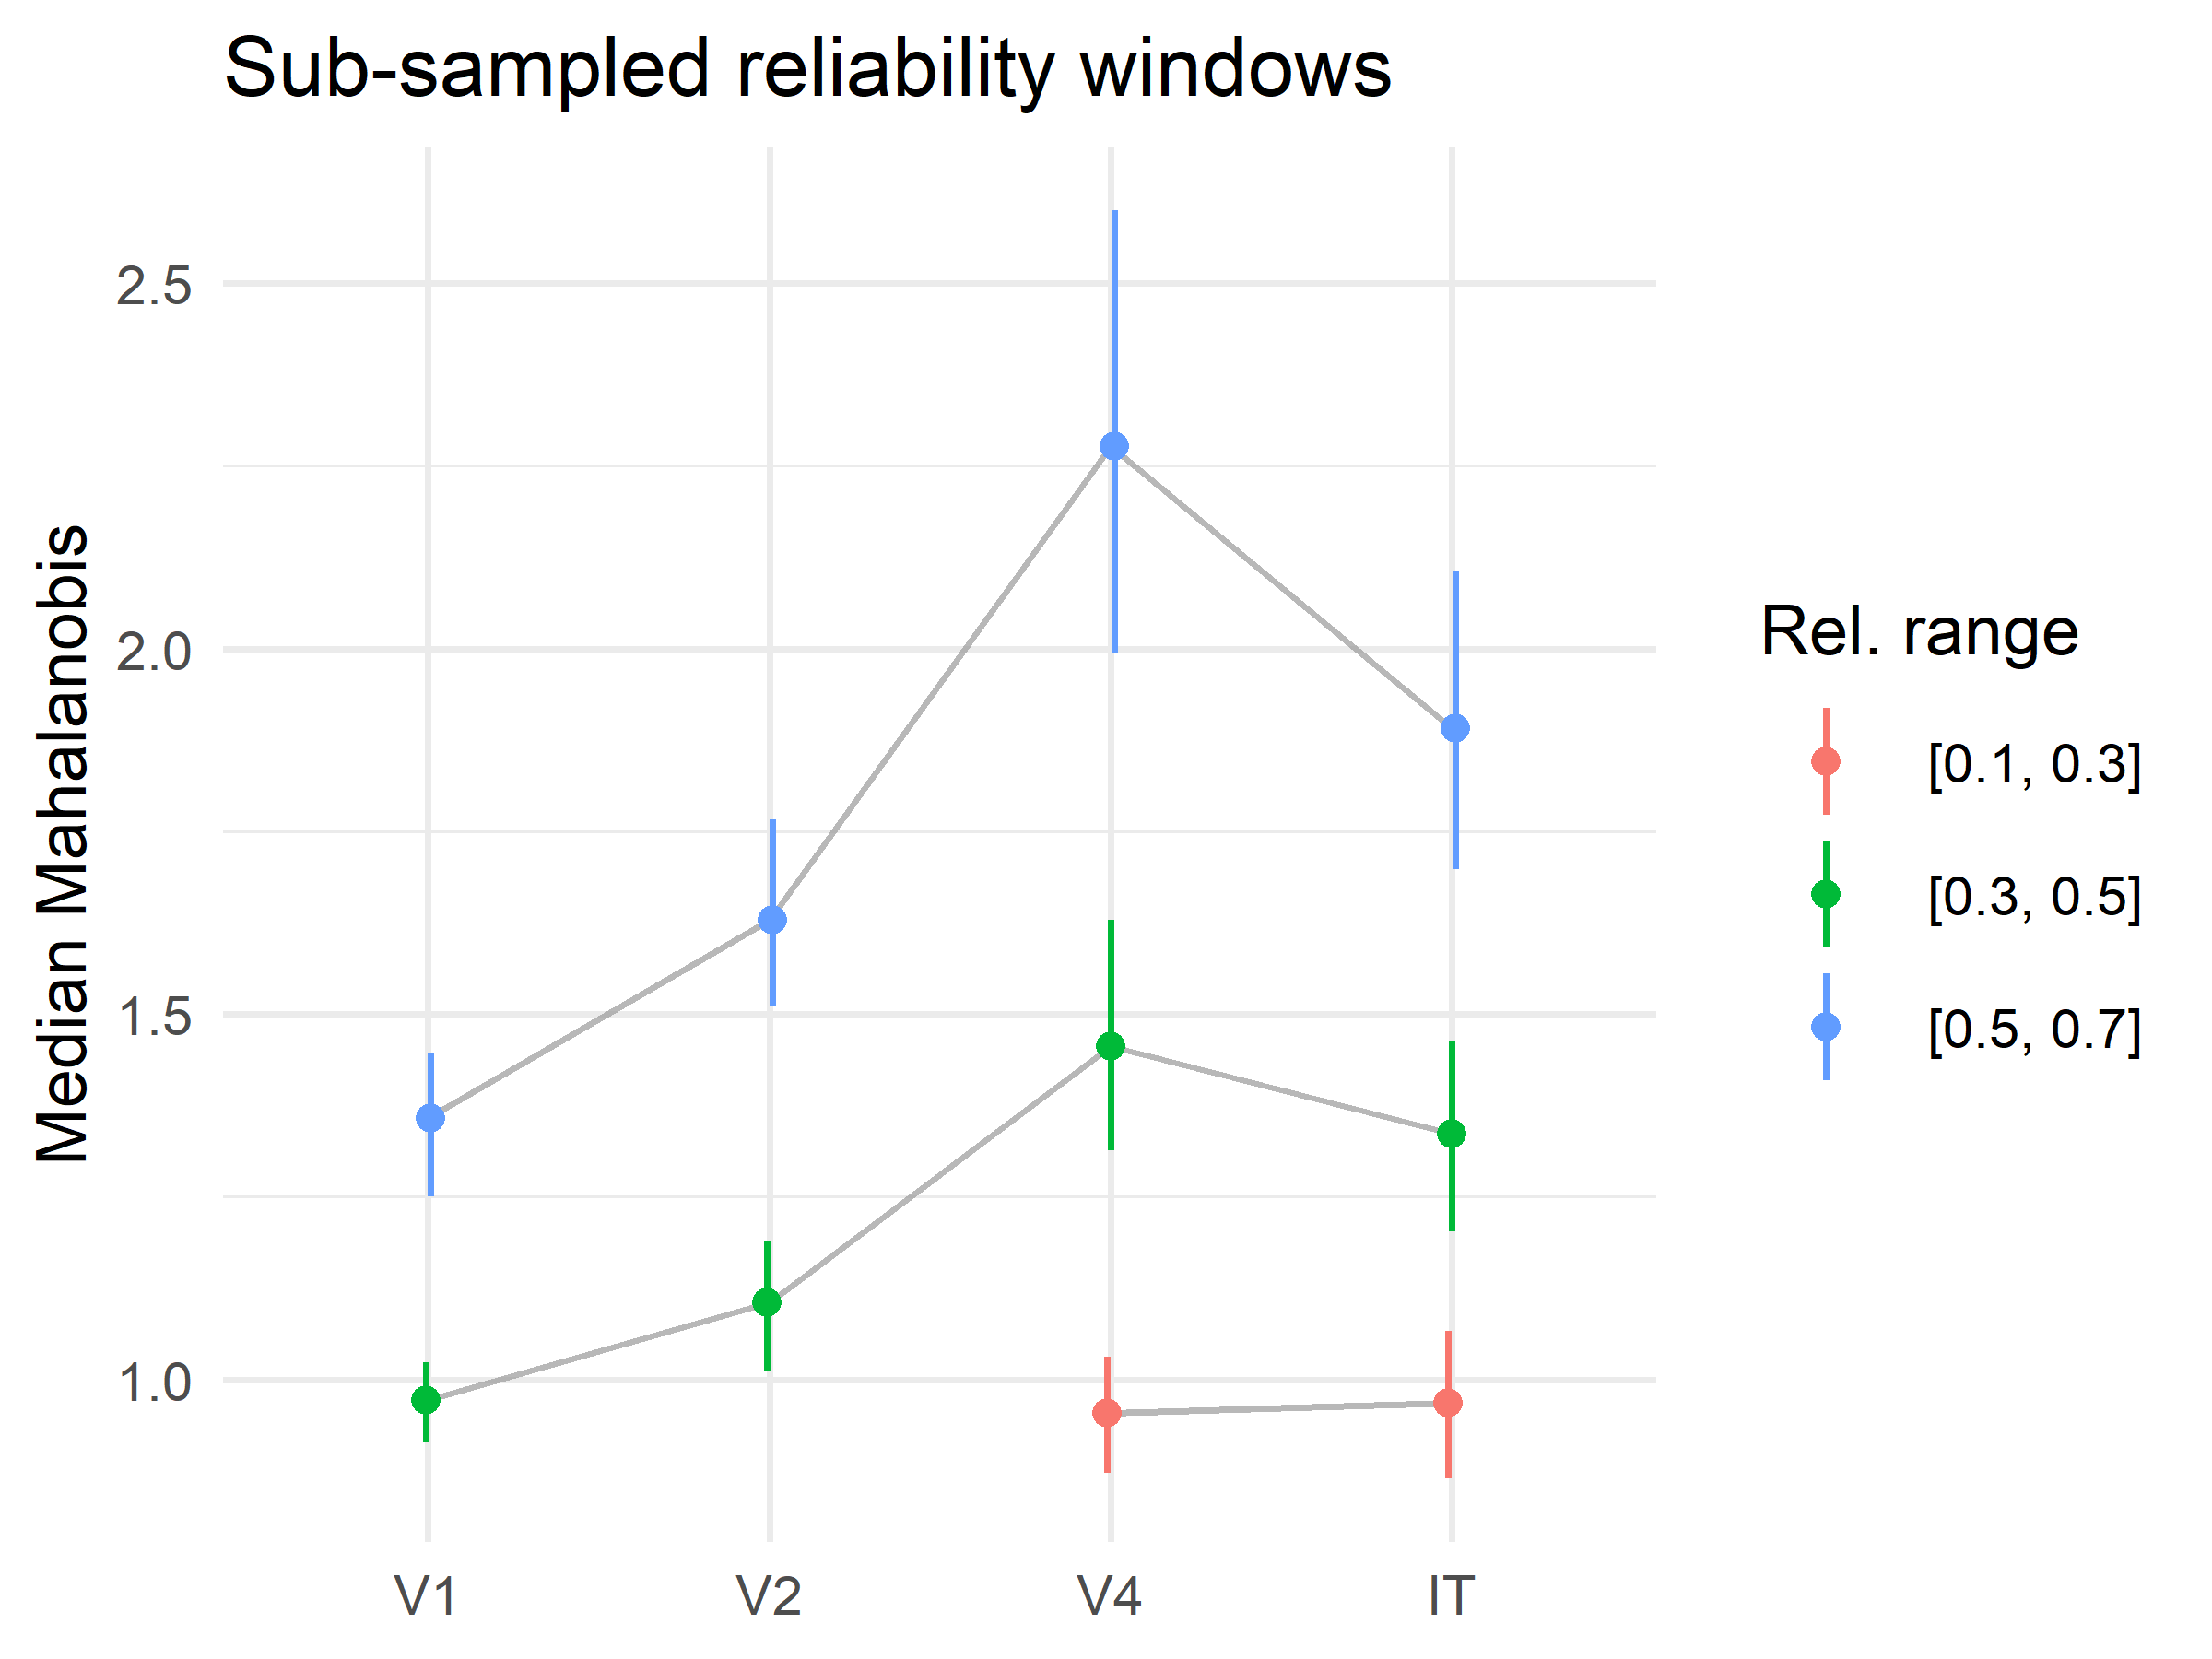
\includegraphics[width=\textwidth]{img/dM_pf_sliding.png} \pause
\end{column}
\begin{column}{0.43\textwidth}
    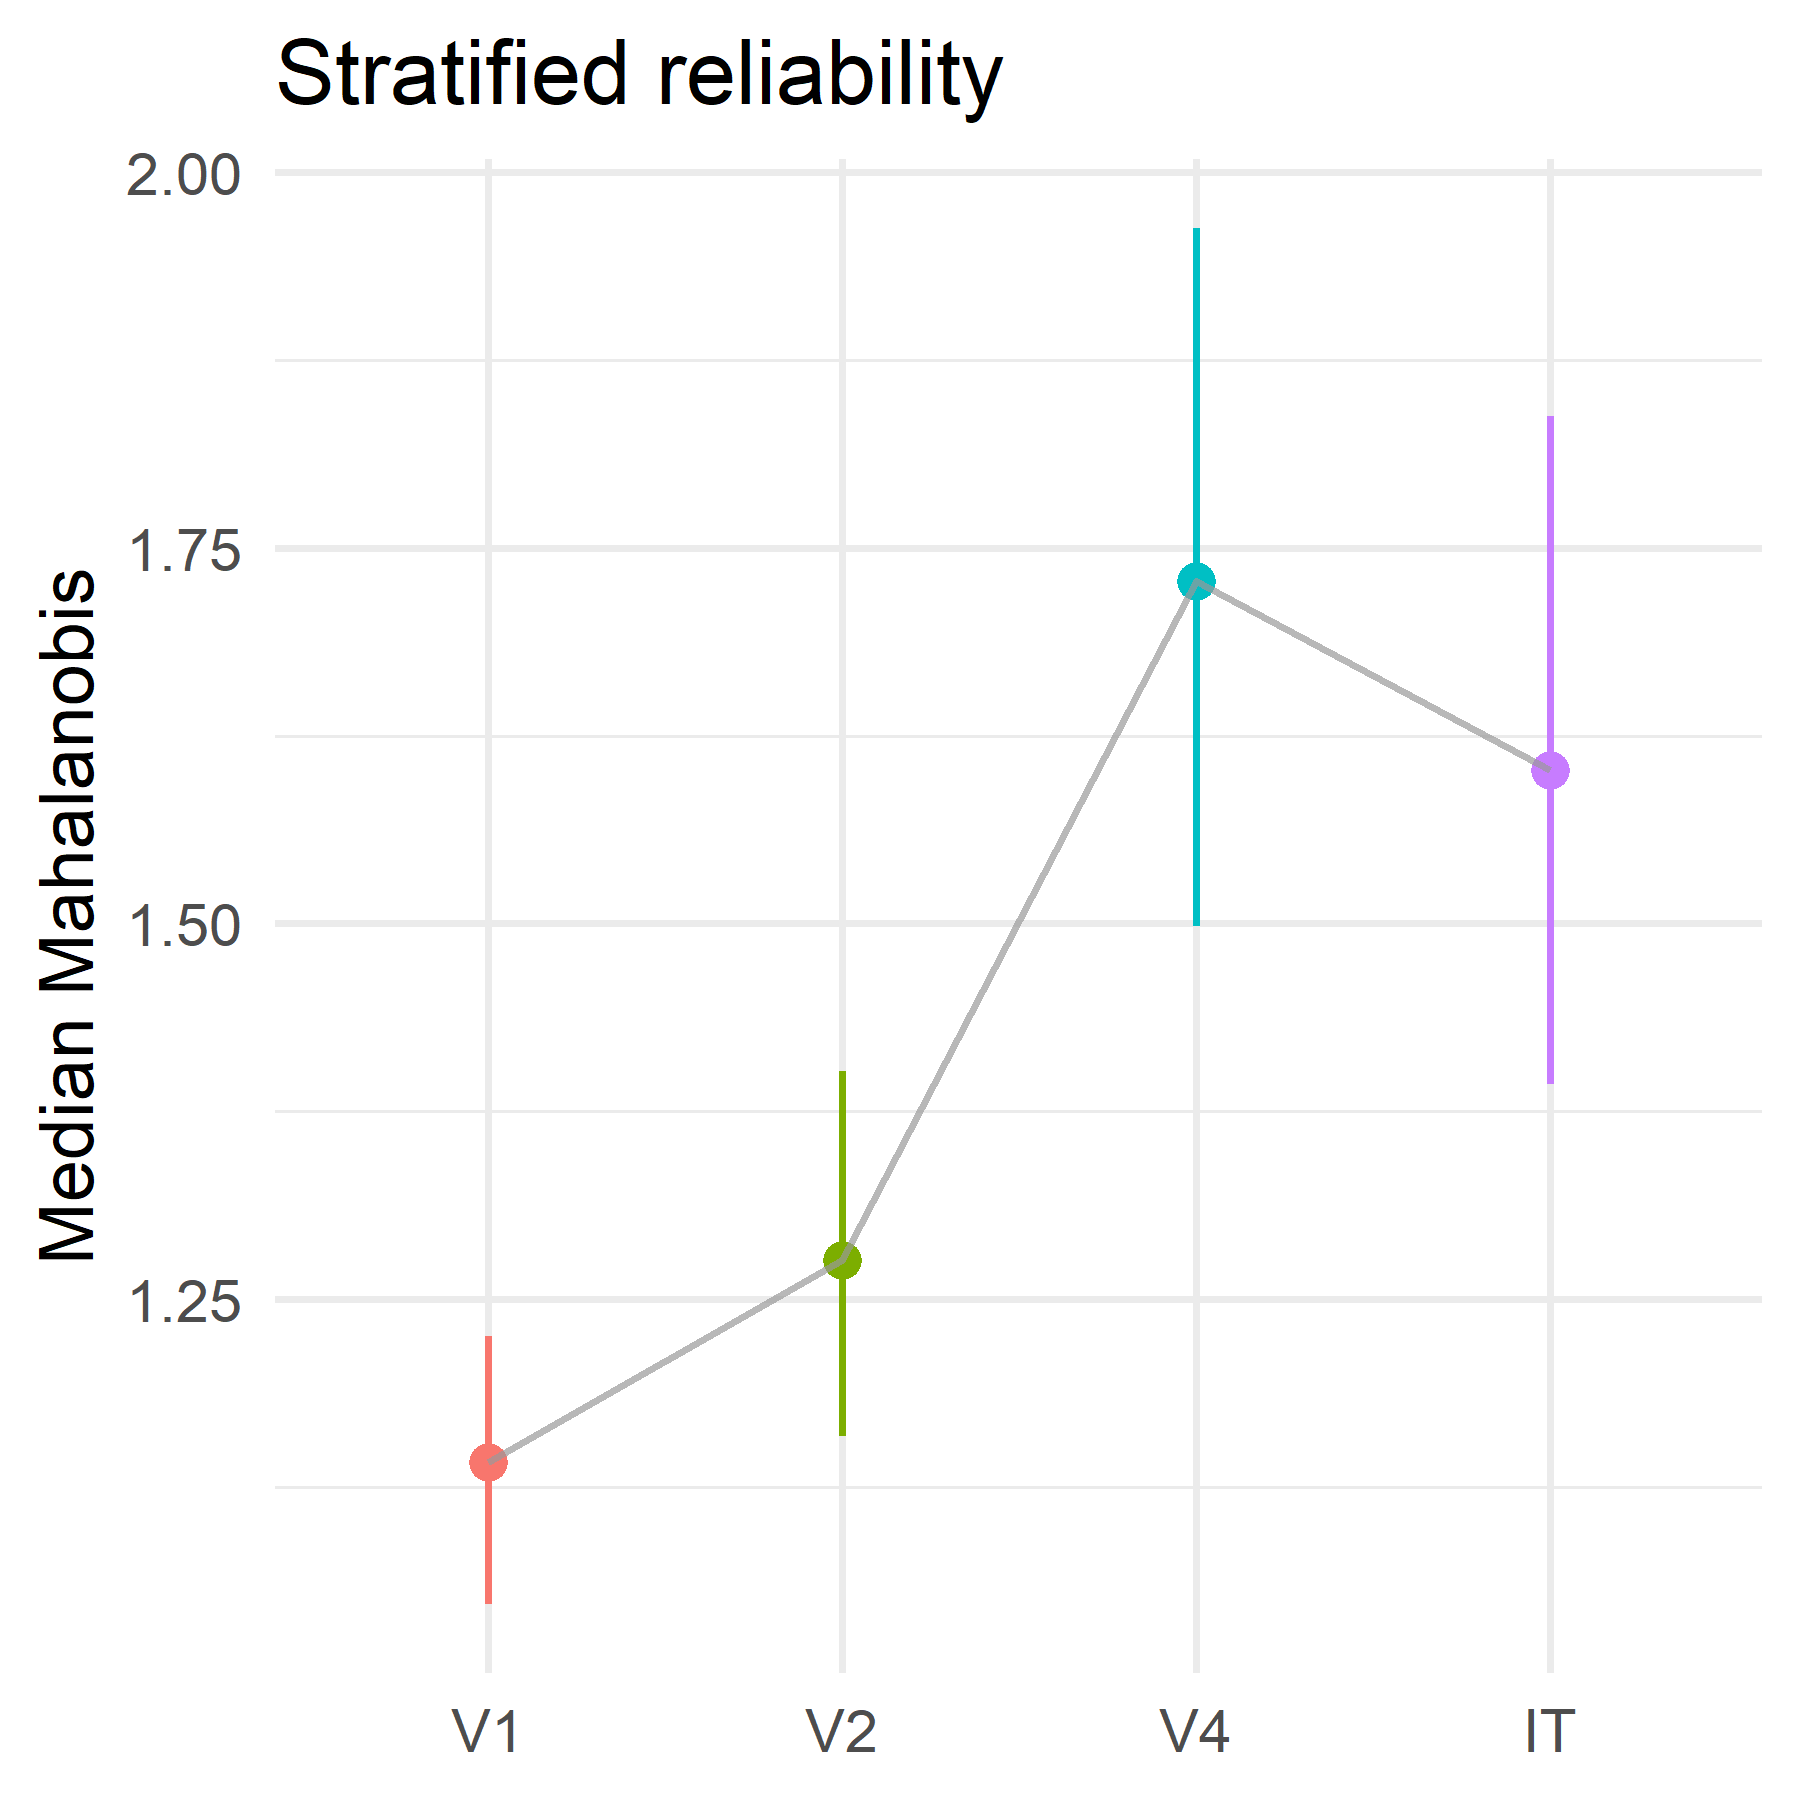
\includegraphics[width=\textwidth]{img/dM_pf_resample.png}
\end{column}
\end{columns}
\end{frame}

% \begin{frame}{Sparsity differences can be explained as a relationship between the mean firing and reliability of a site}
% \todo{TODO: write up the definitional derivation of these curves.}

% \centering
% 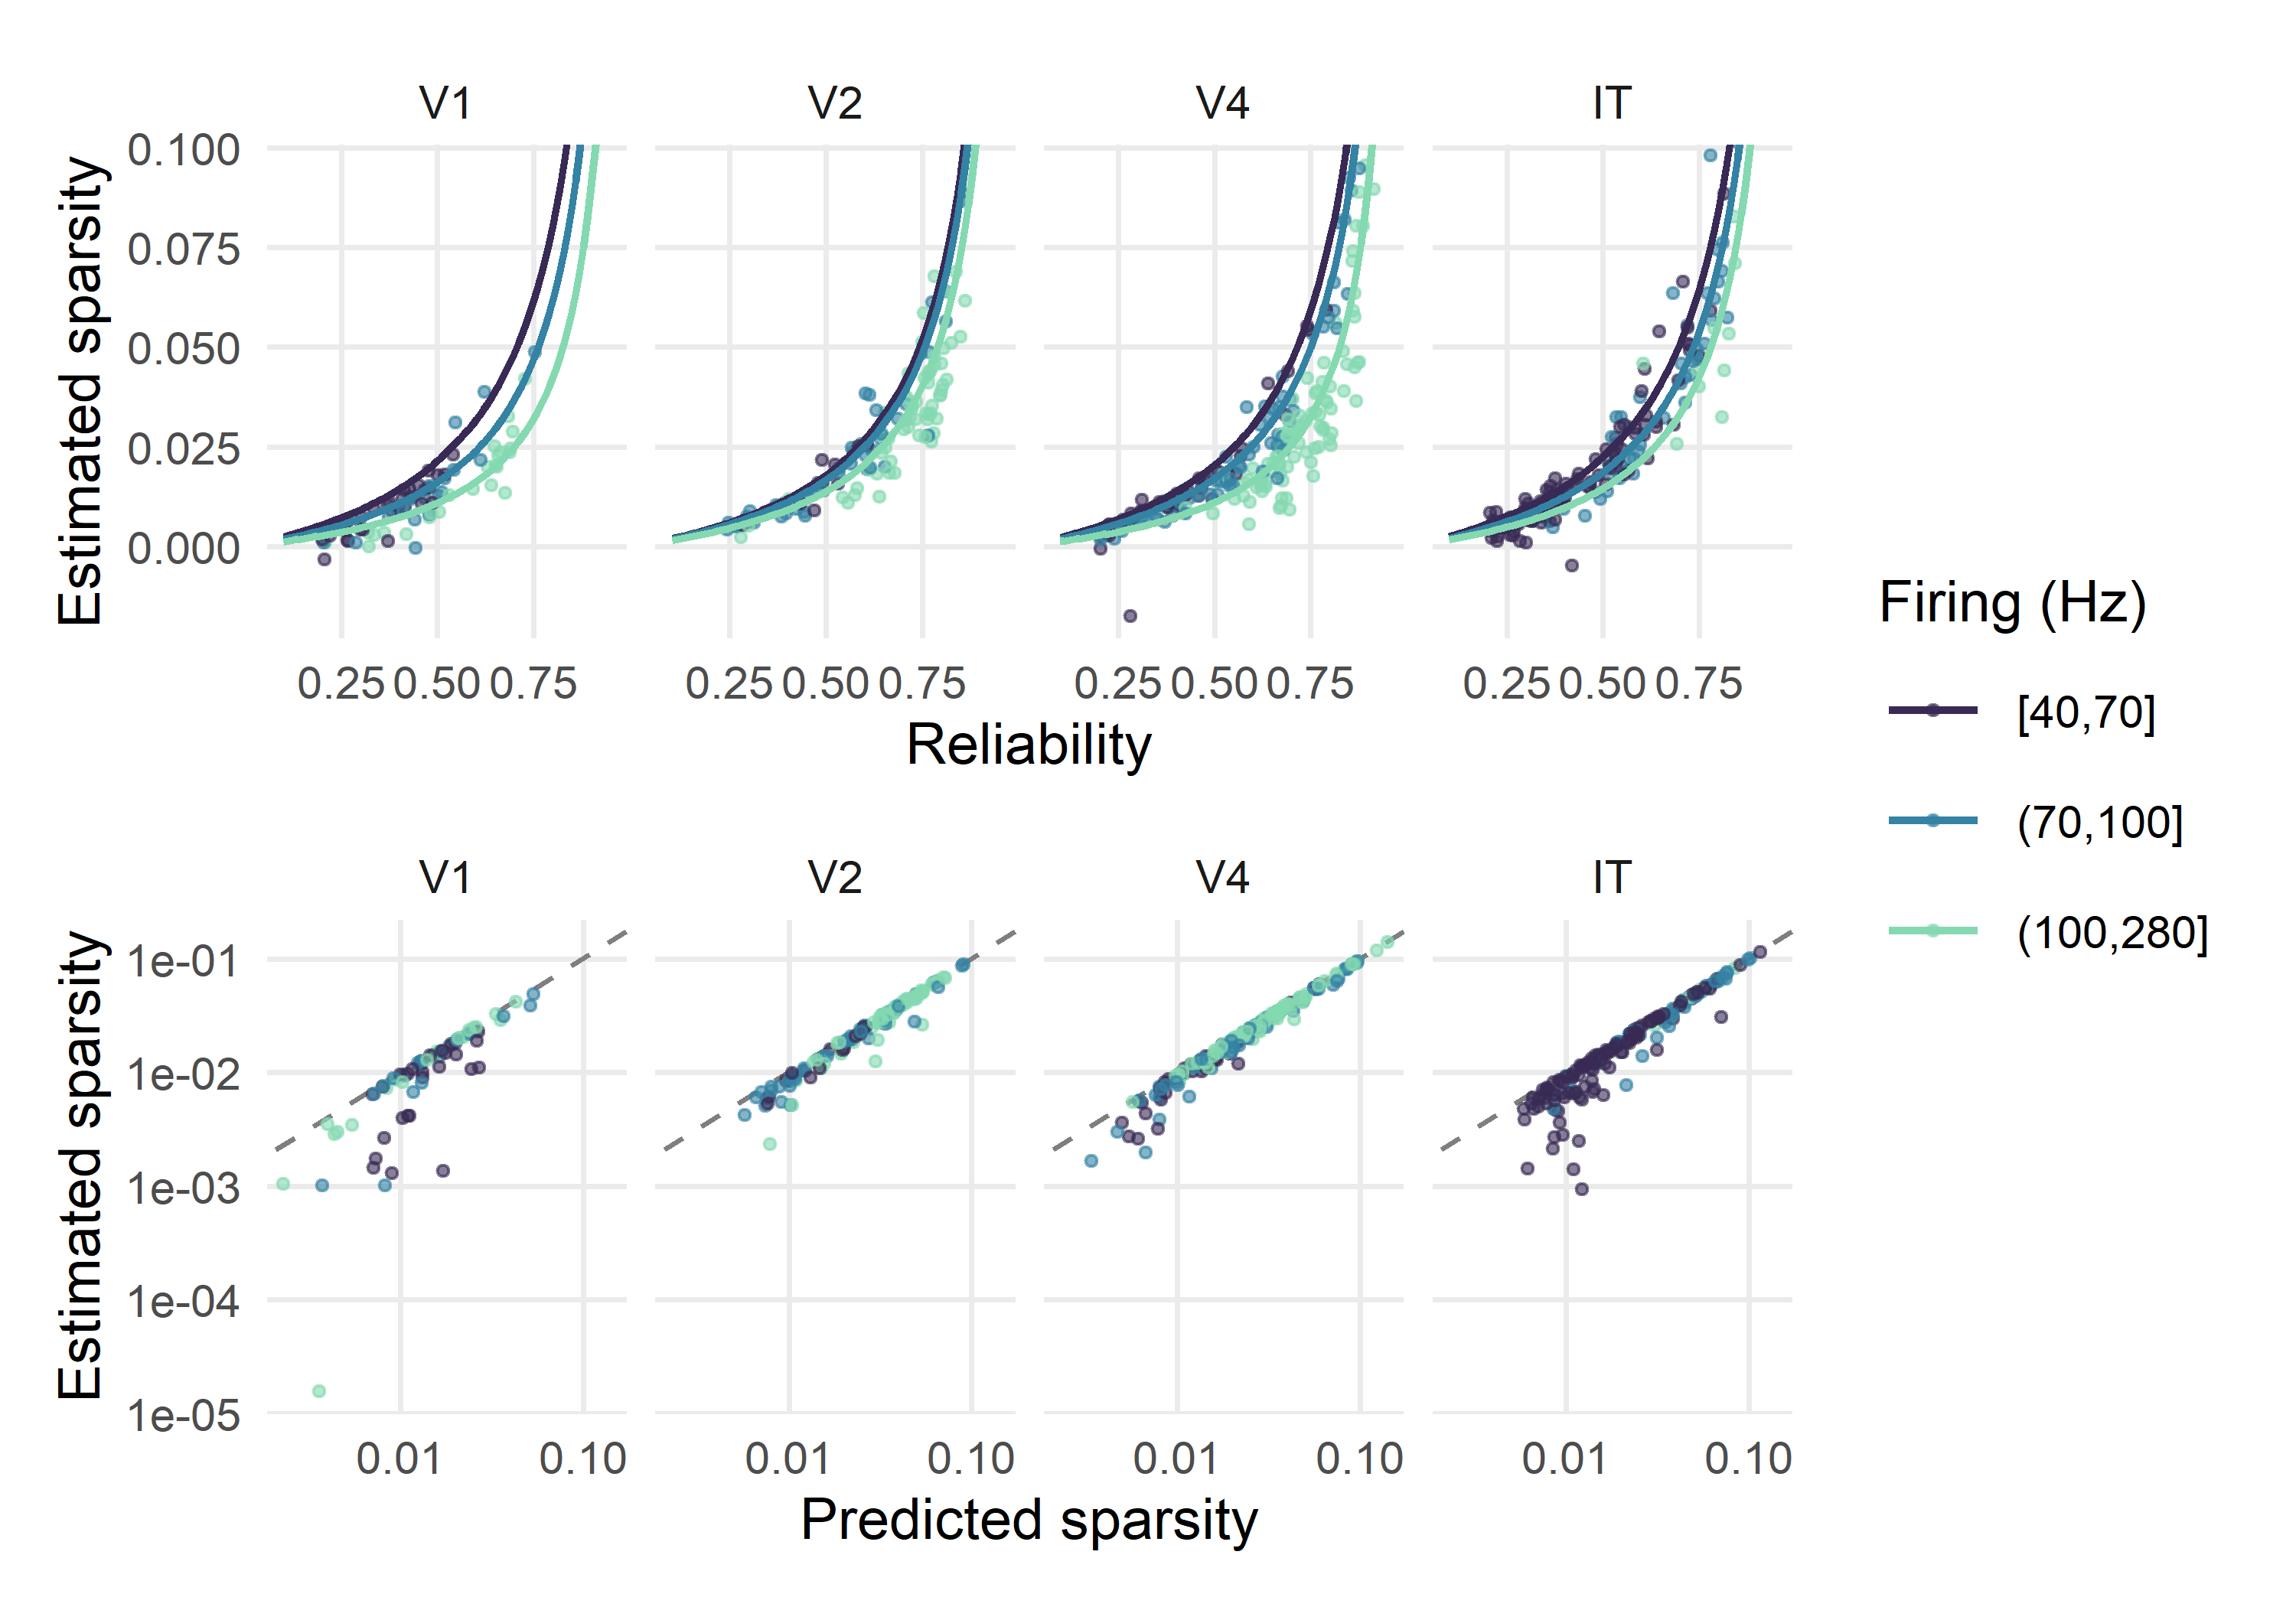
\includegraphics[width=0.7\textwidth]{img/sparsity_rate_reliability.png}
% \end{frame}

% \begin{frame}{Reliability influences the calculated neural separability}
% \centering 
% 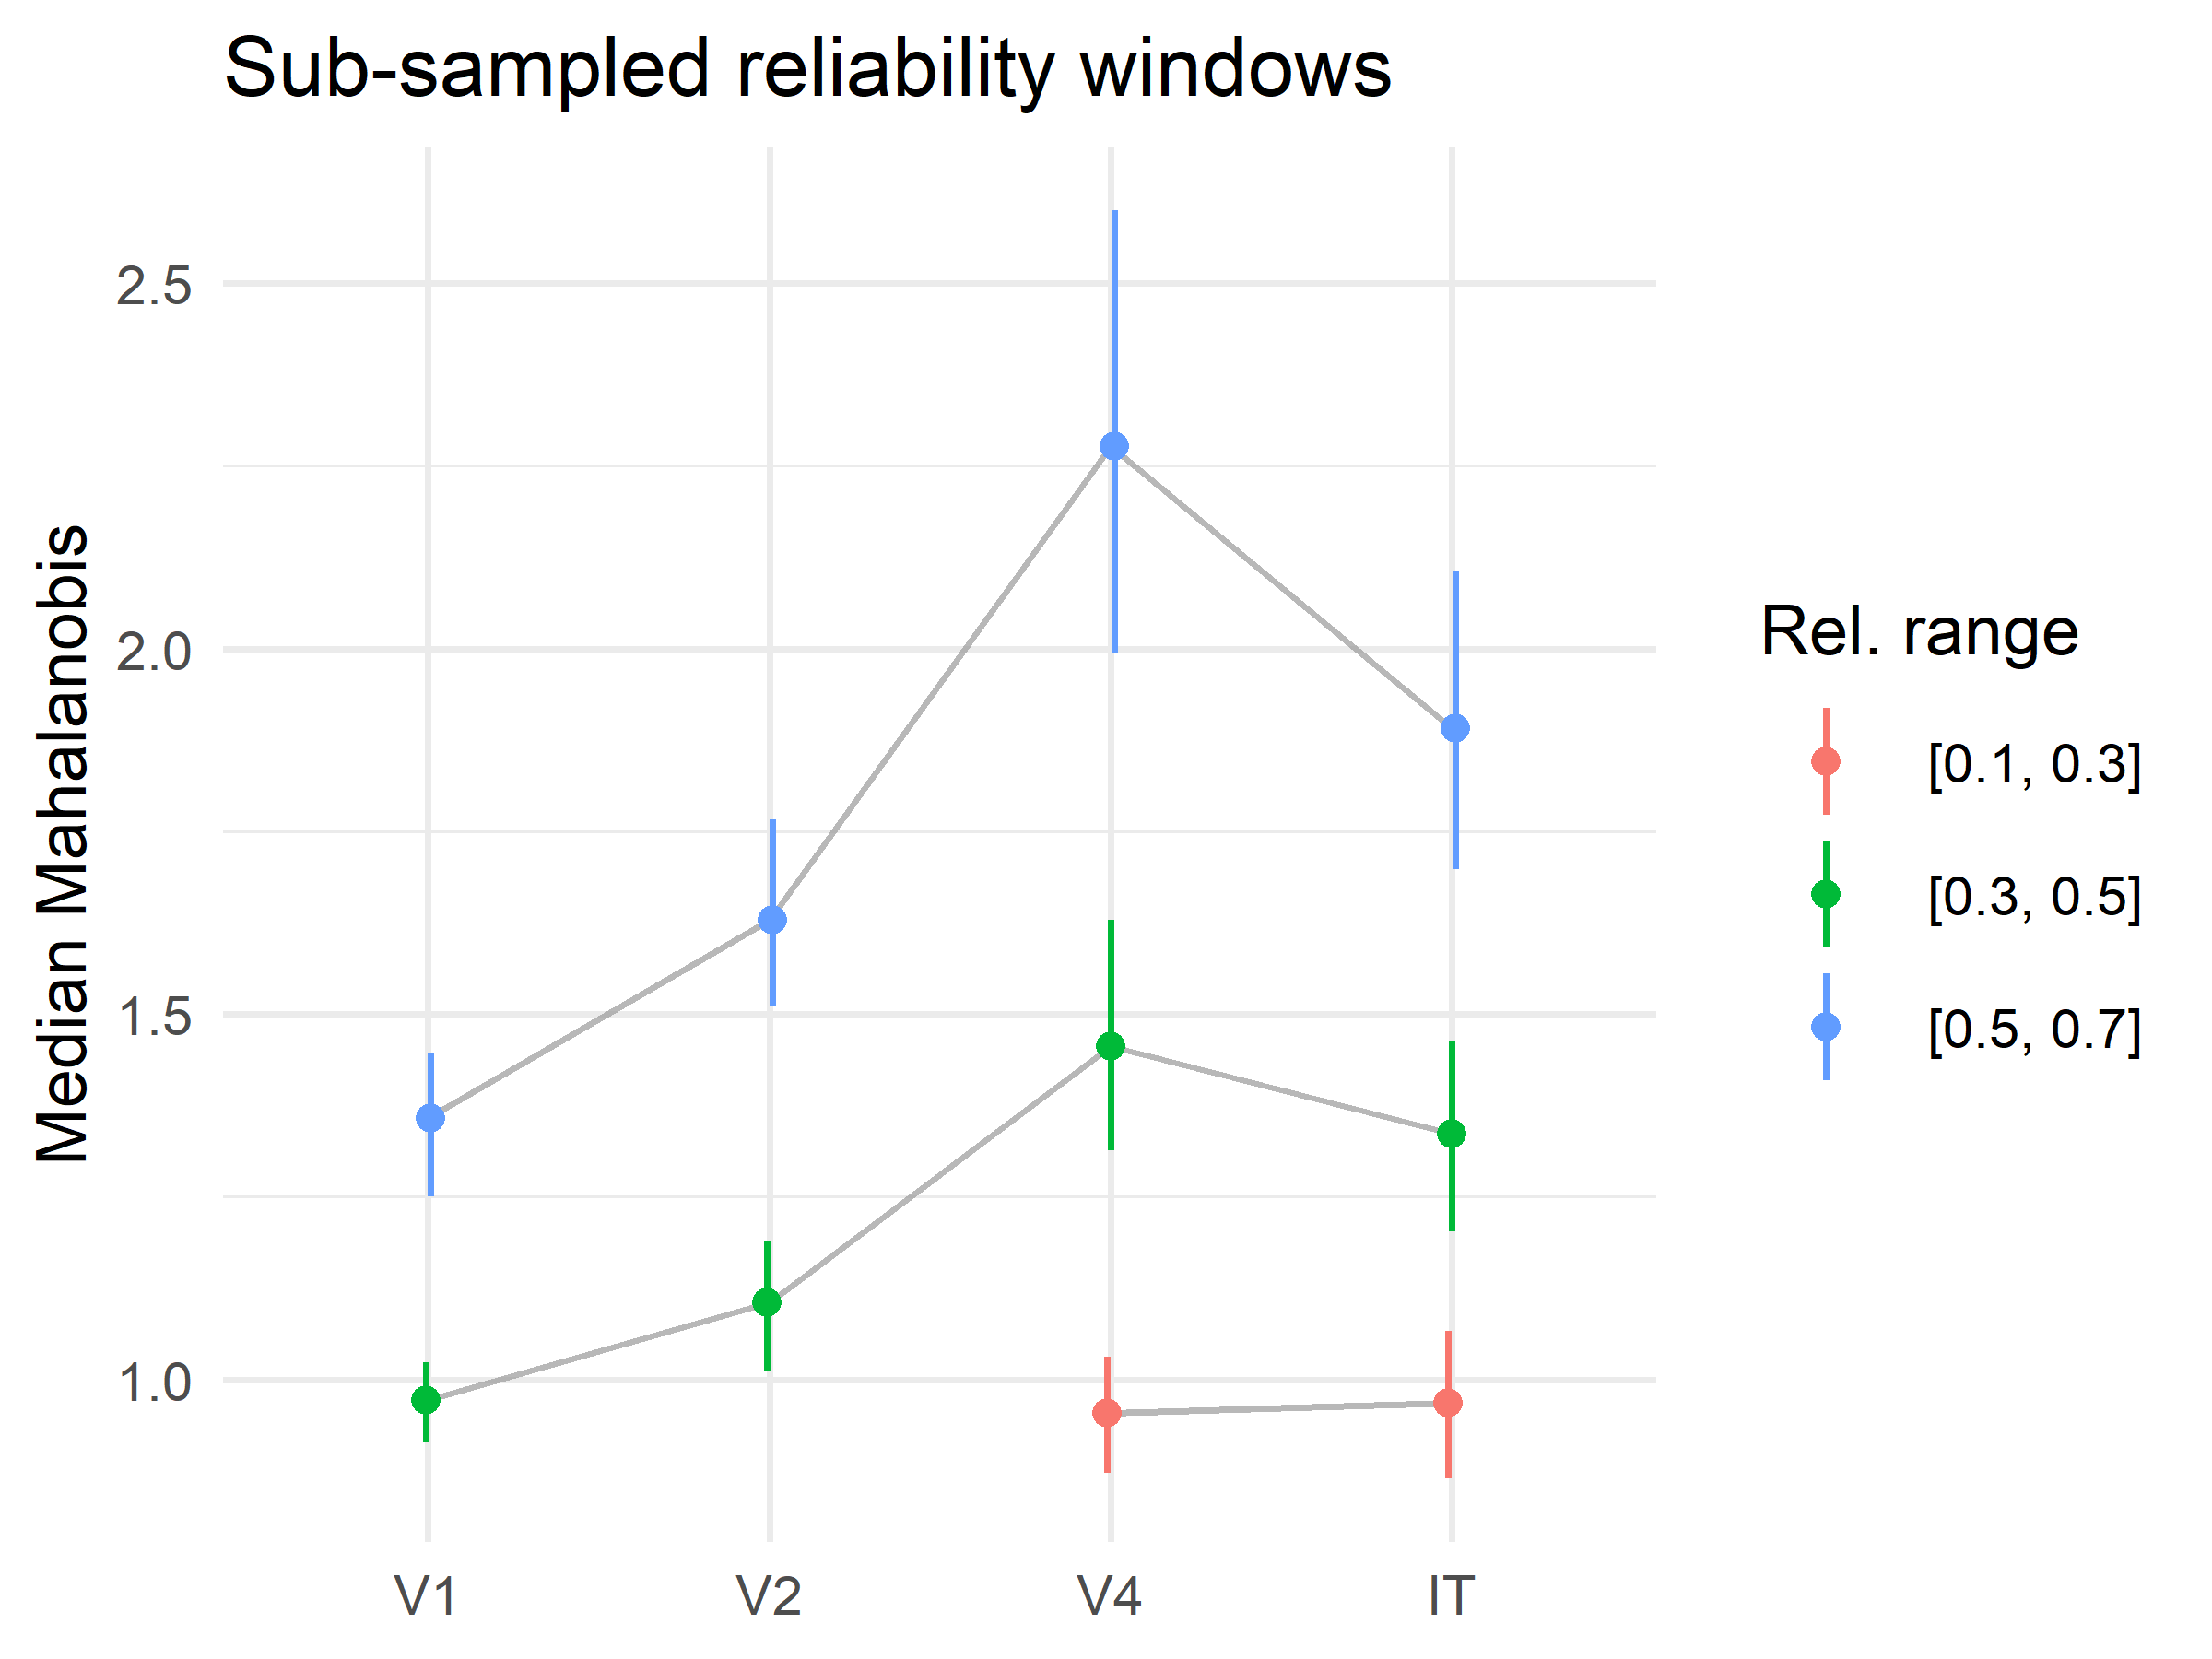
\includegraphics[width=0.8\textwidth]{img/dM_pf_sliding.png}
% \end{frame}

\begin{frame}{The distance trend reverses for between sample comparisons}
\begin{columns}
\begin{column}{0.6\textwidth}
\begin{itemize}
    \item Each point represents the between-sample comparisons within a family \pause 
    \item Instead of \( \hat{D}_{\textrm{sample}} \), report ratio of mean \( \hat{D}^2_{\textrm{sample}} \) within a family to mean \( \hat{D}^2_{\textrm{out-fam}}\) \pause 
    \item Ratio \( \approx 1 \): images within family are as different as images across families \pause 
\end{itemize}
\end{column}
\begin{column}{0.4\textwidth}
    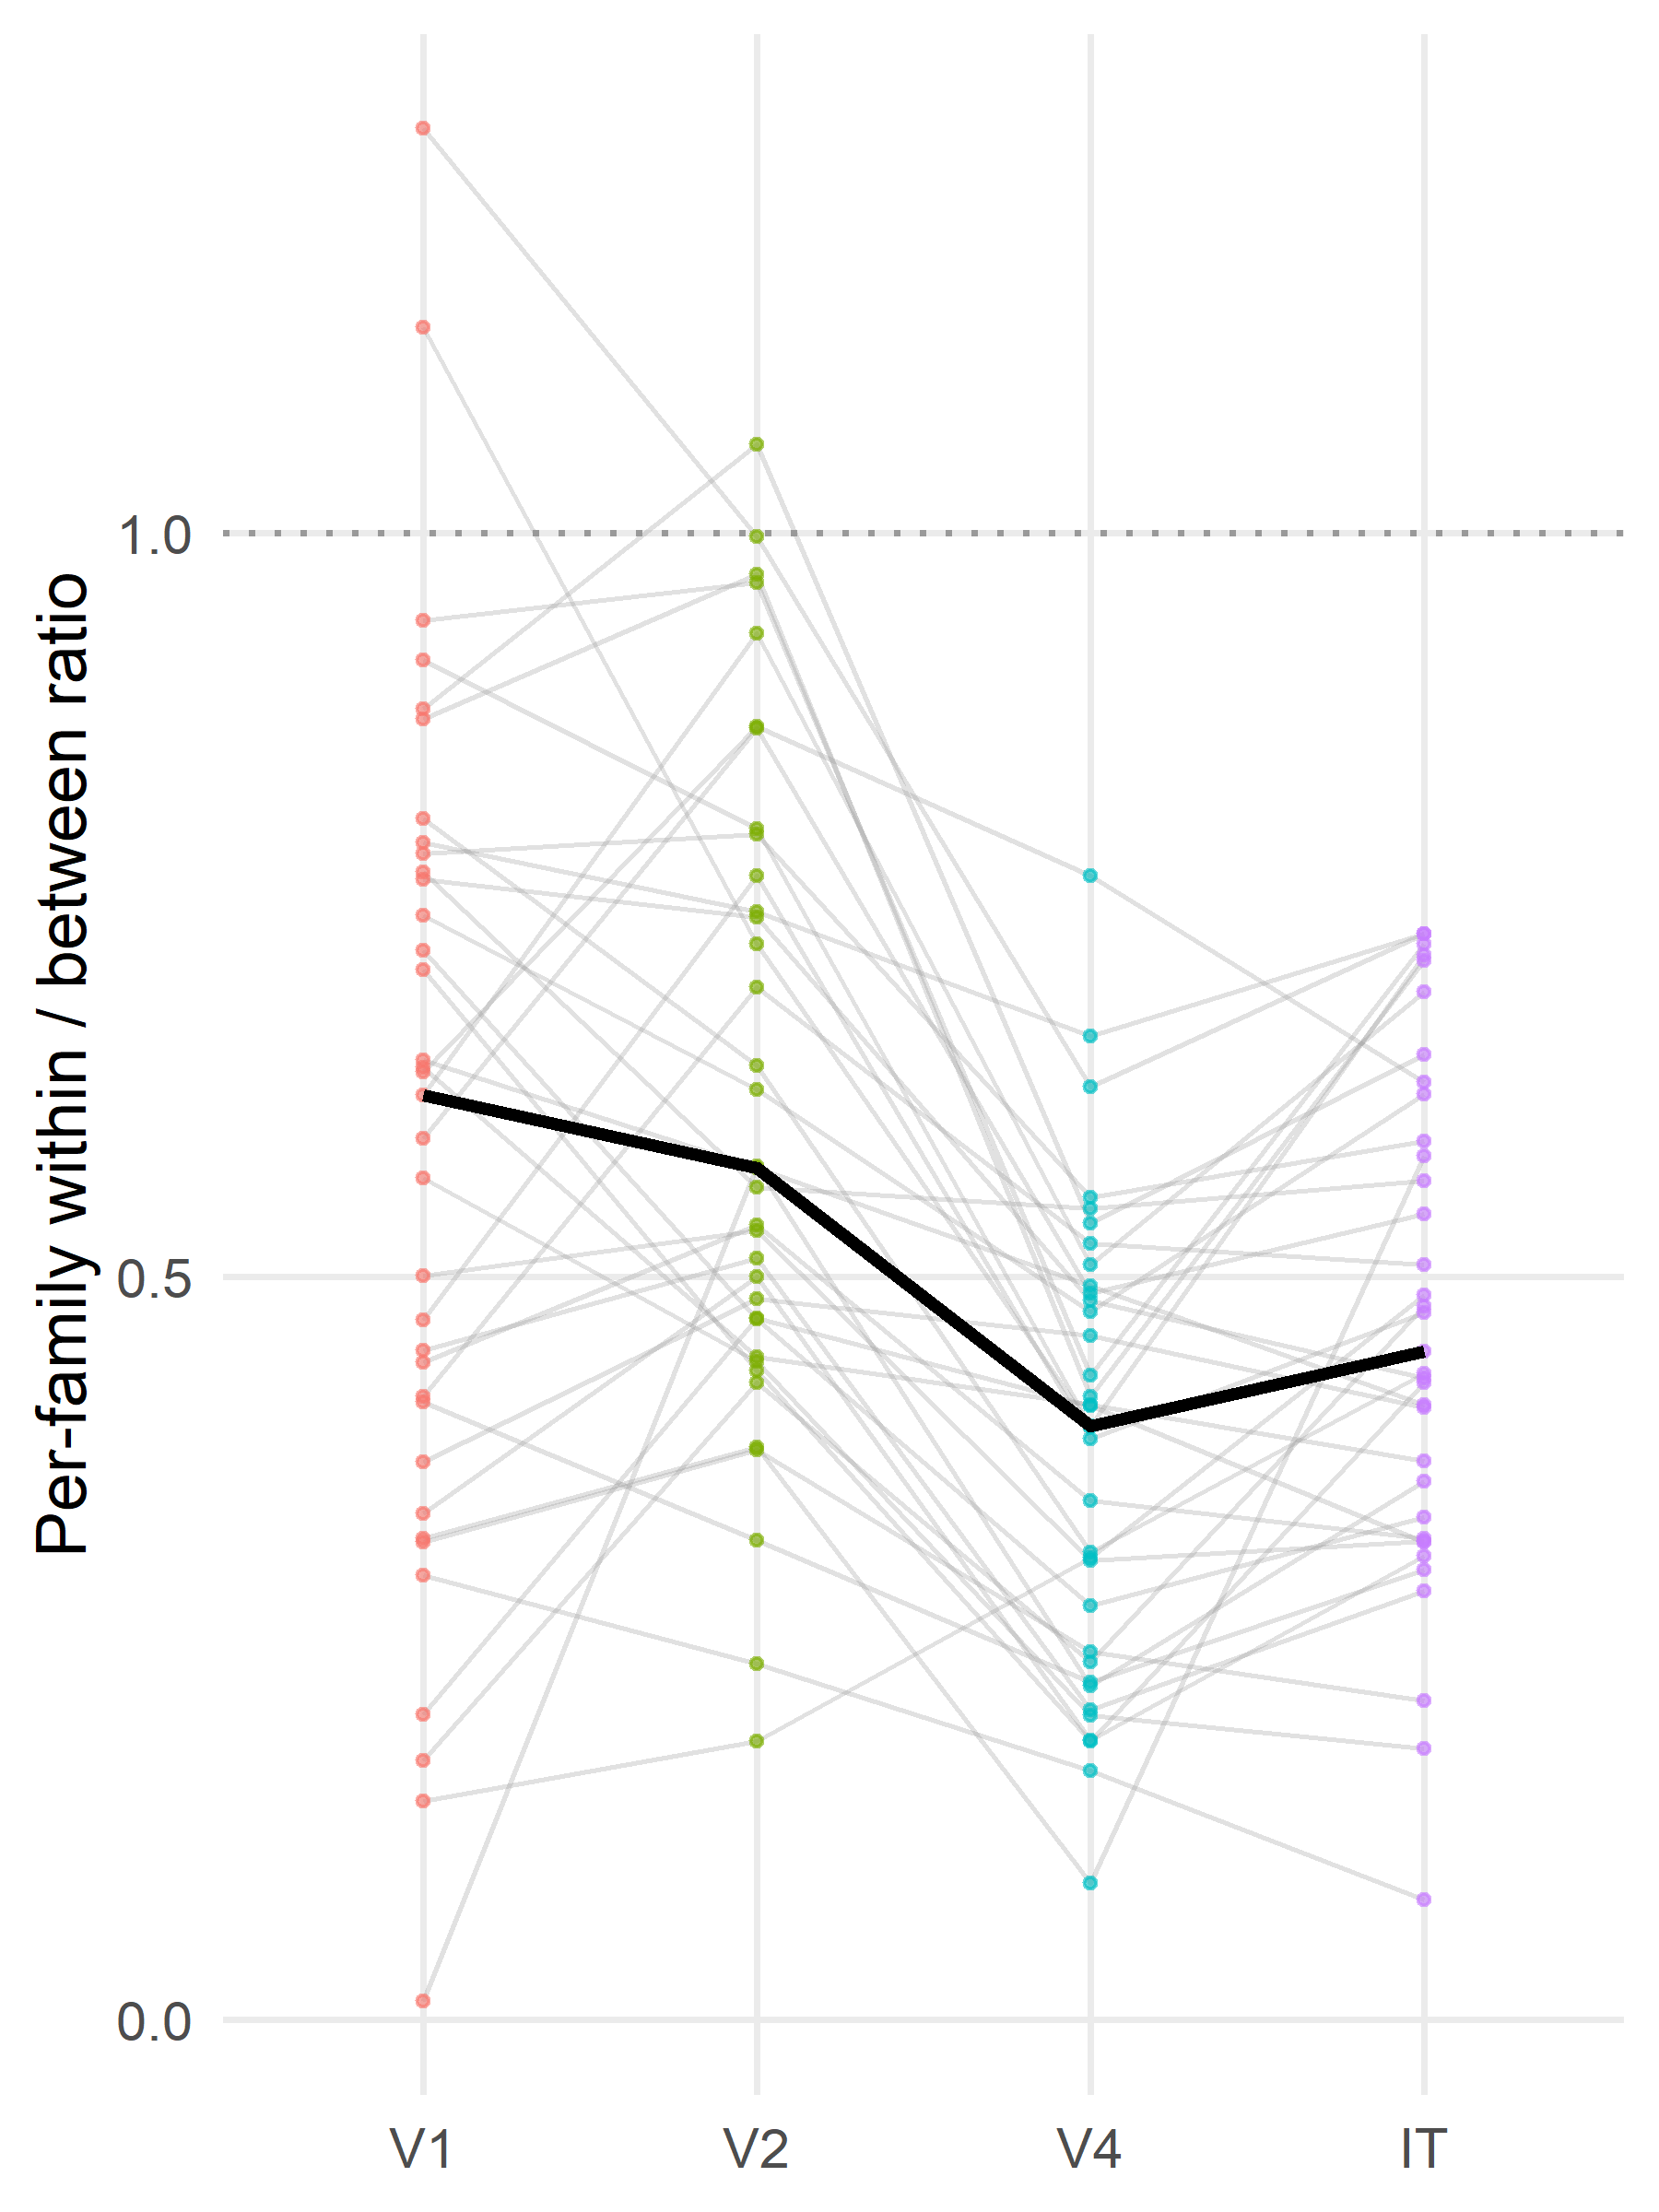
\includegraphics[width=\textwidth]{img/dM_ps_ratio.png}
\end{column}
\end{columns}
\end{frame}

% \begin{frame}{The results are consistent with a hierarchical ANOVA}
%     \todo{TODO}
% \end{frame}

\begin{frame}{Discussion}
\begin{columns}
\begin{column}{0.35\textwidth}
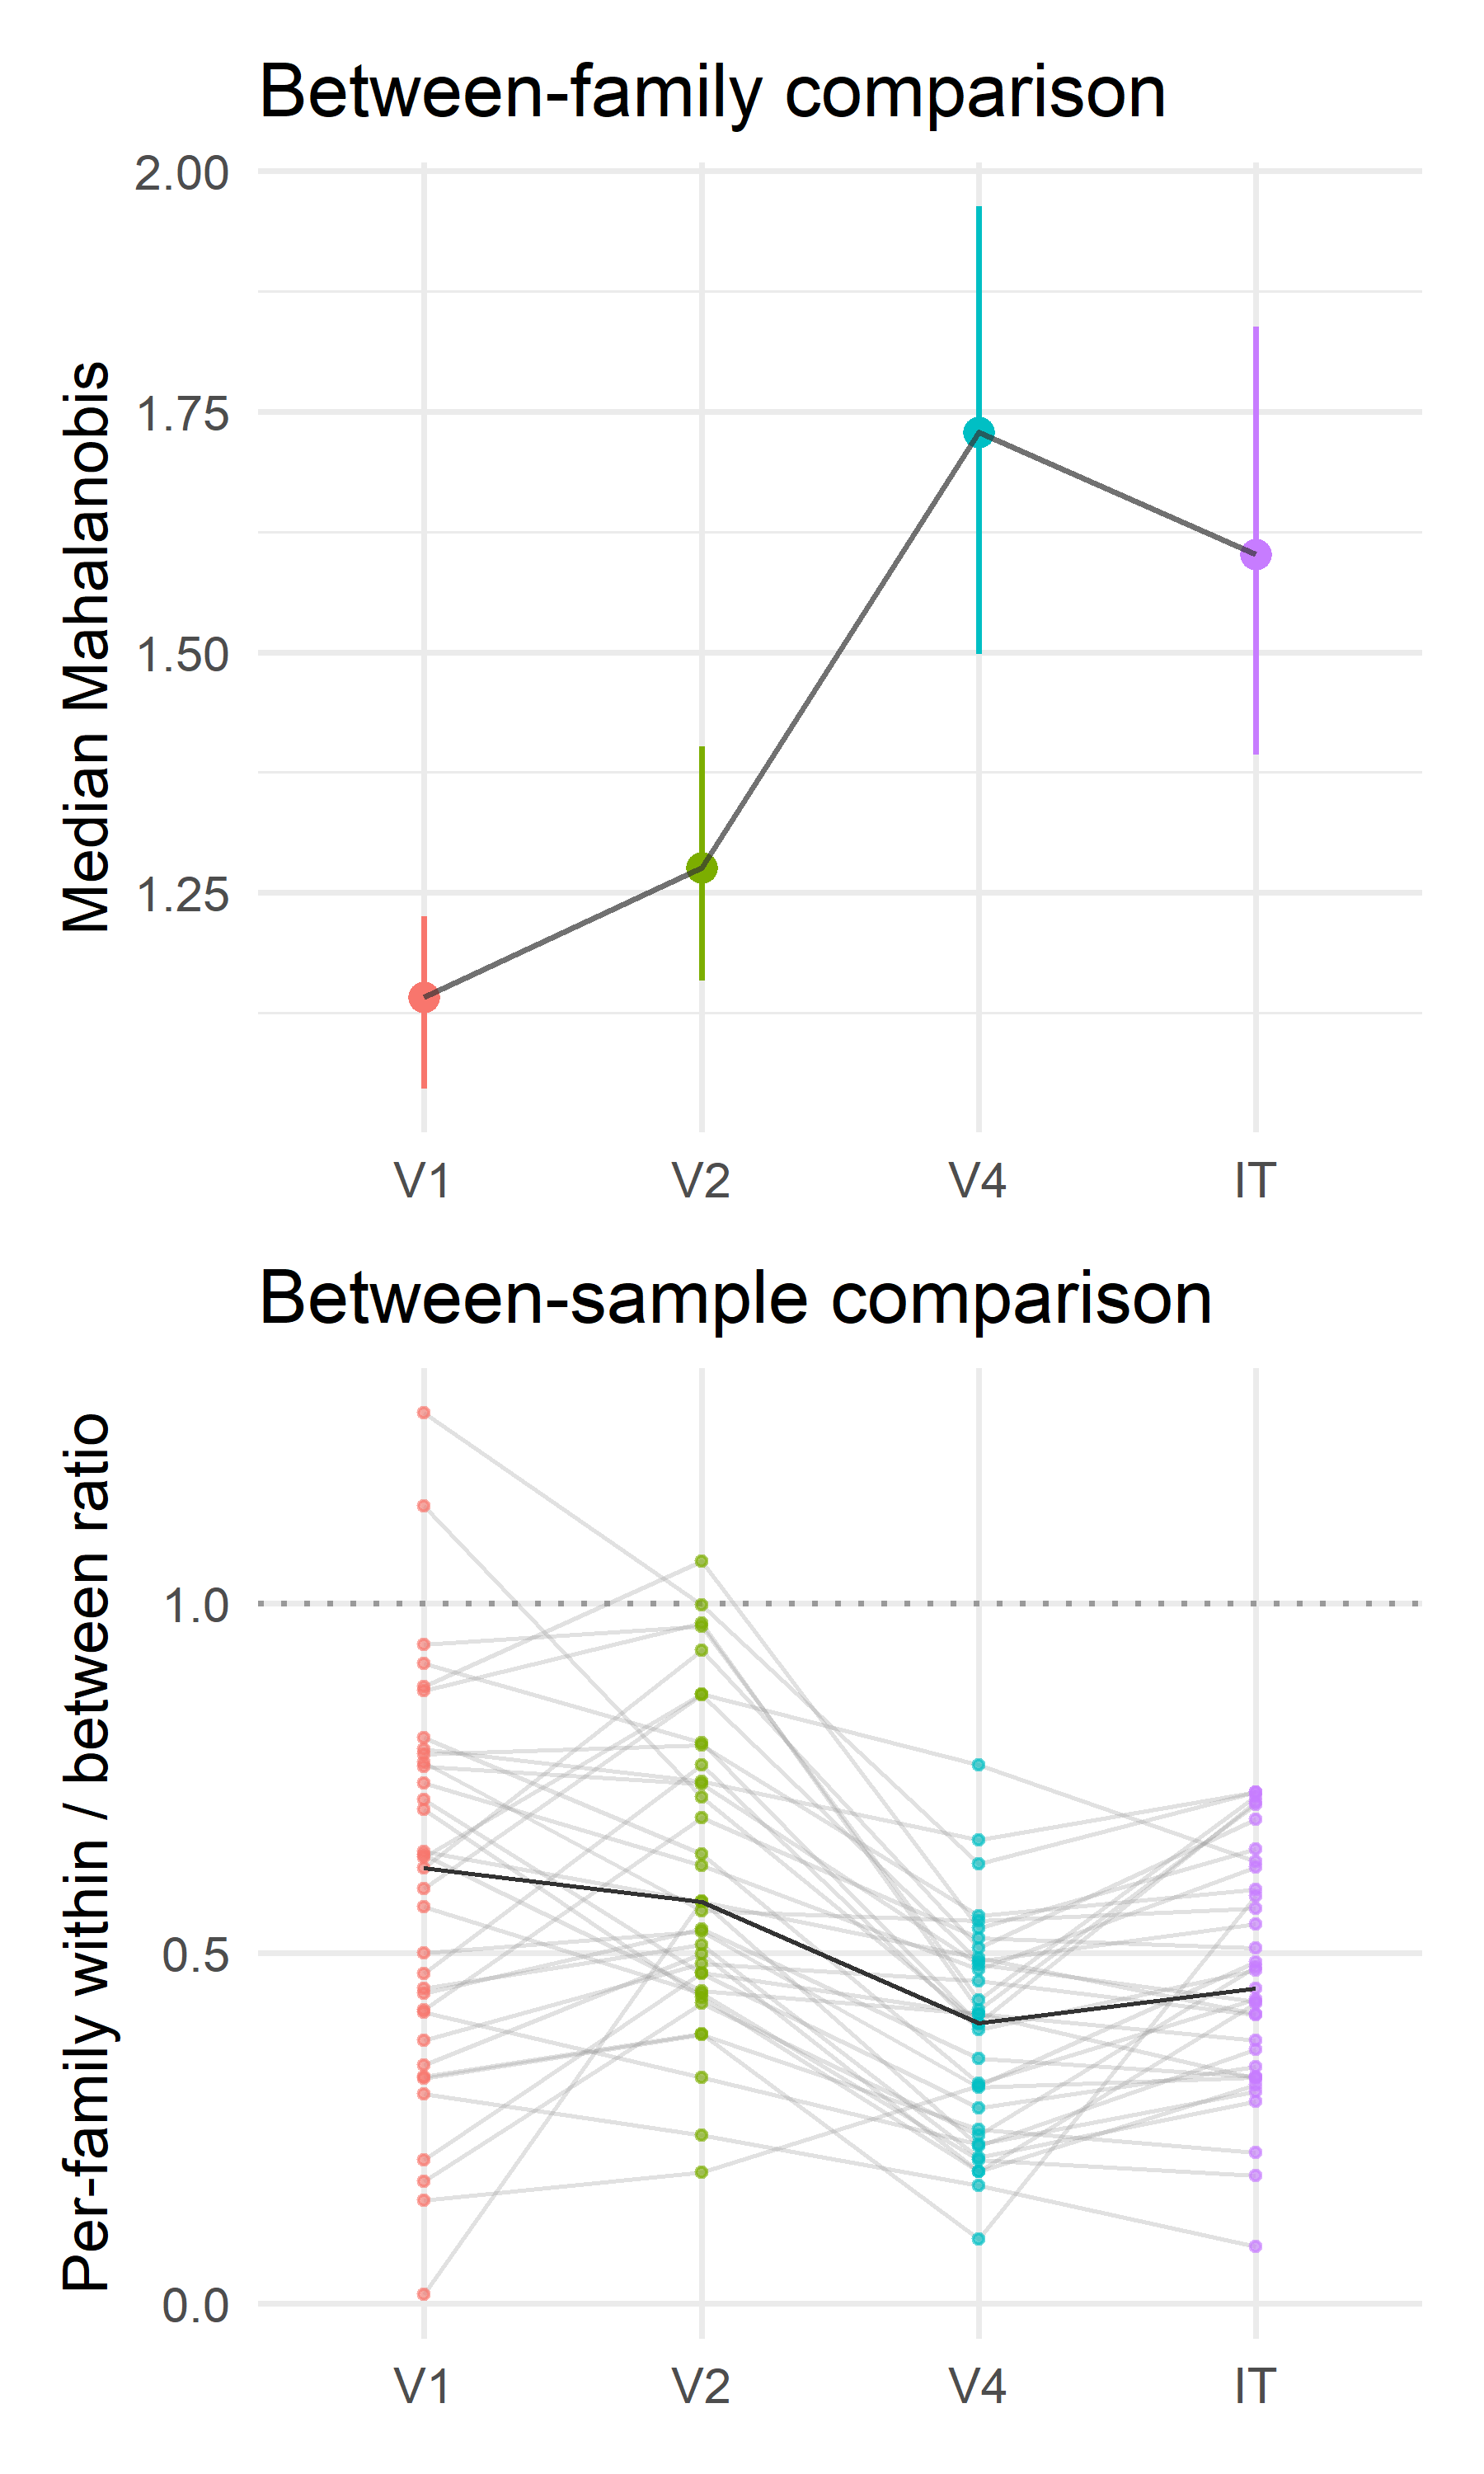
\includegraphics[width=\textwidth]{img/pf_ps_summary.png}
\end{column}
\begin{column}{0.65\textwidth}
\begin{itemize}
    \item V1 and V2 results agree with literature \parencite{ziemba_selectivity_2016}
    \item Not a clear increase from V1 to IT, though in general, later areas separate families better. \pause 
    \item Between-sample variance is difficult to visualize at only 6 repetitions. \pause  
    % \item Debiased sparsity estimators tend to agree. When used in their plug-in form, more disagreement arises (especially in low reliability). 
    % \item Instead of per-site sparsity, another comparison of interest would be population sparsity \pause
    \item Multi-unit activations might bias results; higher regions might show weaker spatial correlations \parencite{smith_spatial_2013}. \pause 
    \item Different arrays in the same region might not be a reasonable population to subsample from. 
\end{itemize}
\end{column}
\end{columns}

\end{frame}

\begin{frame}{Thank you and acknowledgments}
\begin{columns}
\begin{column}{0.65\textwidth}
\begin{itemize}
    \item Thank you to my committee and everyone in attendance!
    \item Special acknowledgment to Gerrick Lee (currently a post-doc at UC Berkeley) for data collection and providing additional information
\end{itemize}
\end{column}
\begin{column}{0.35\textwidth}
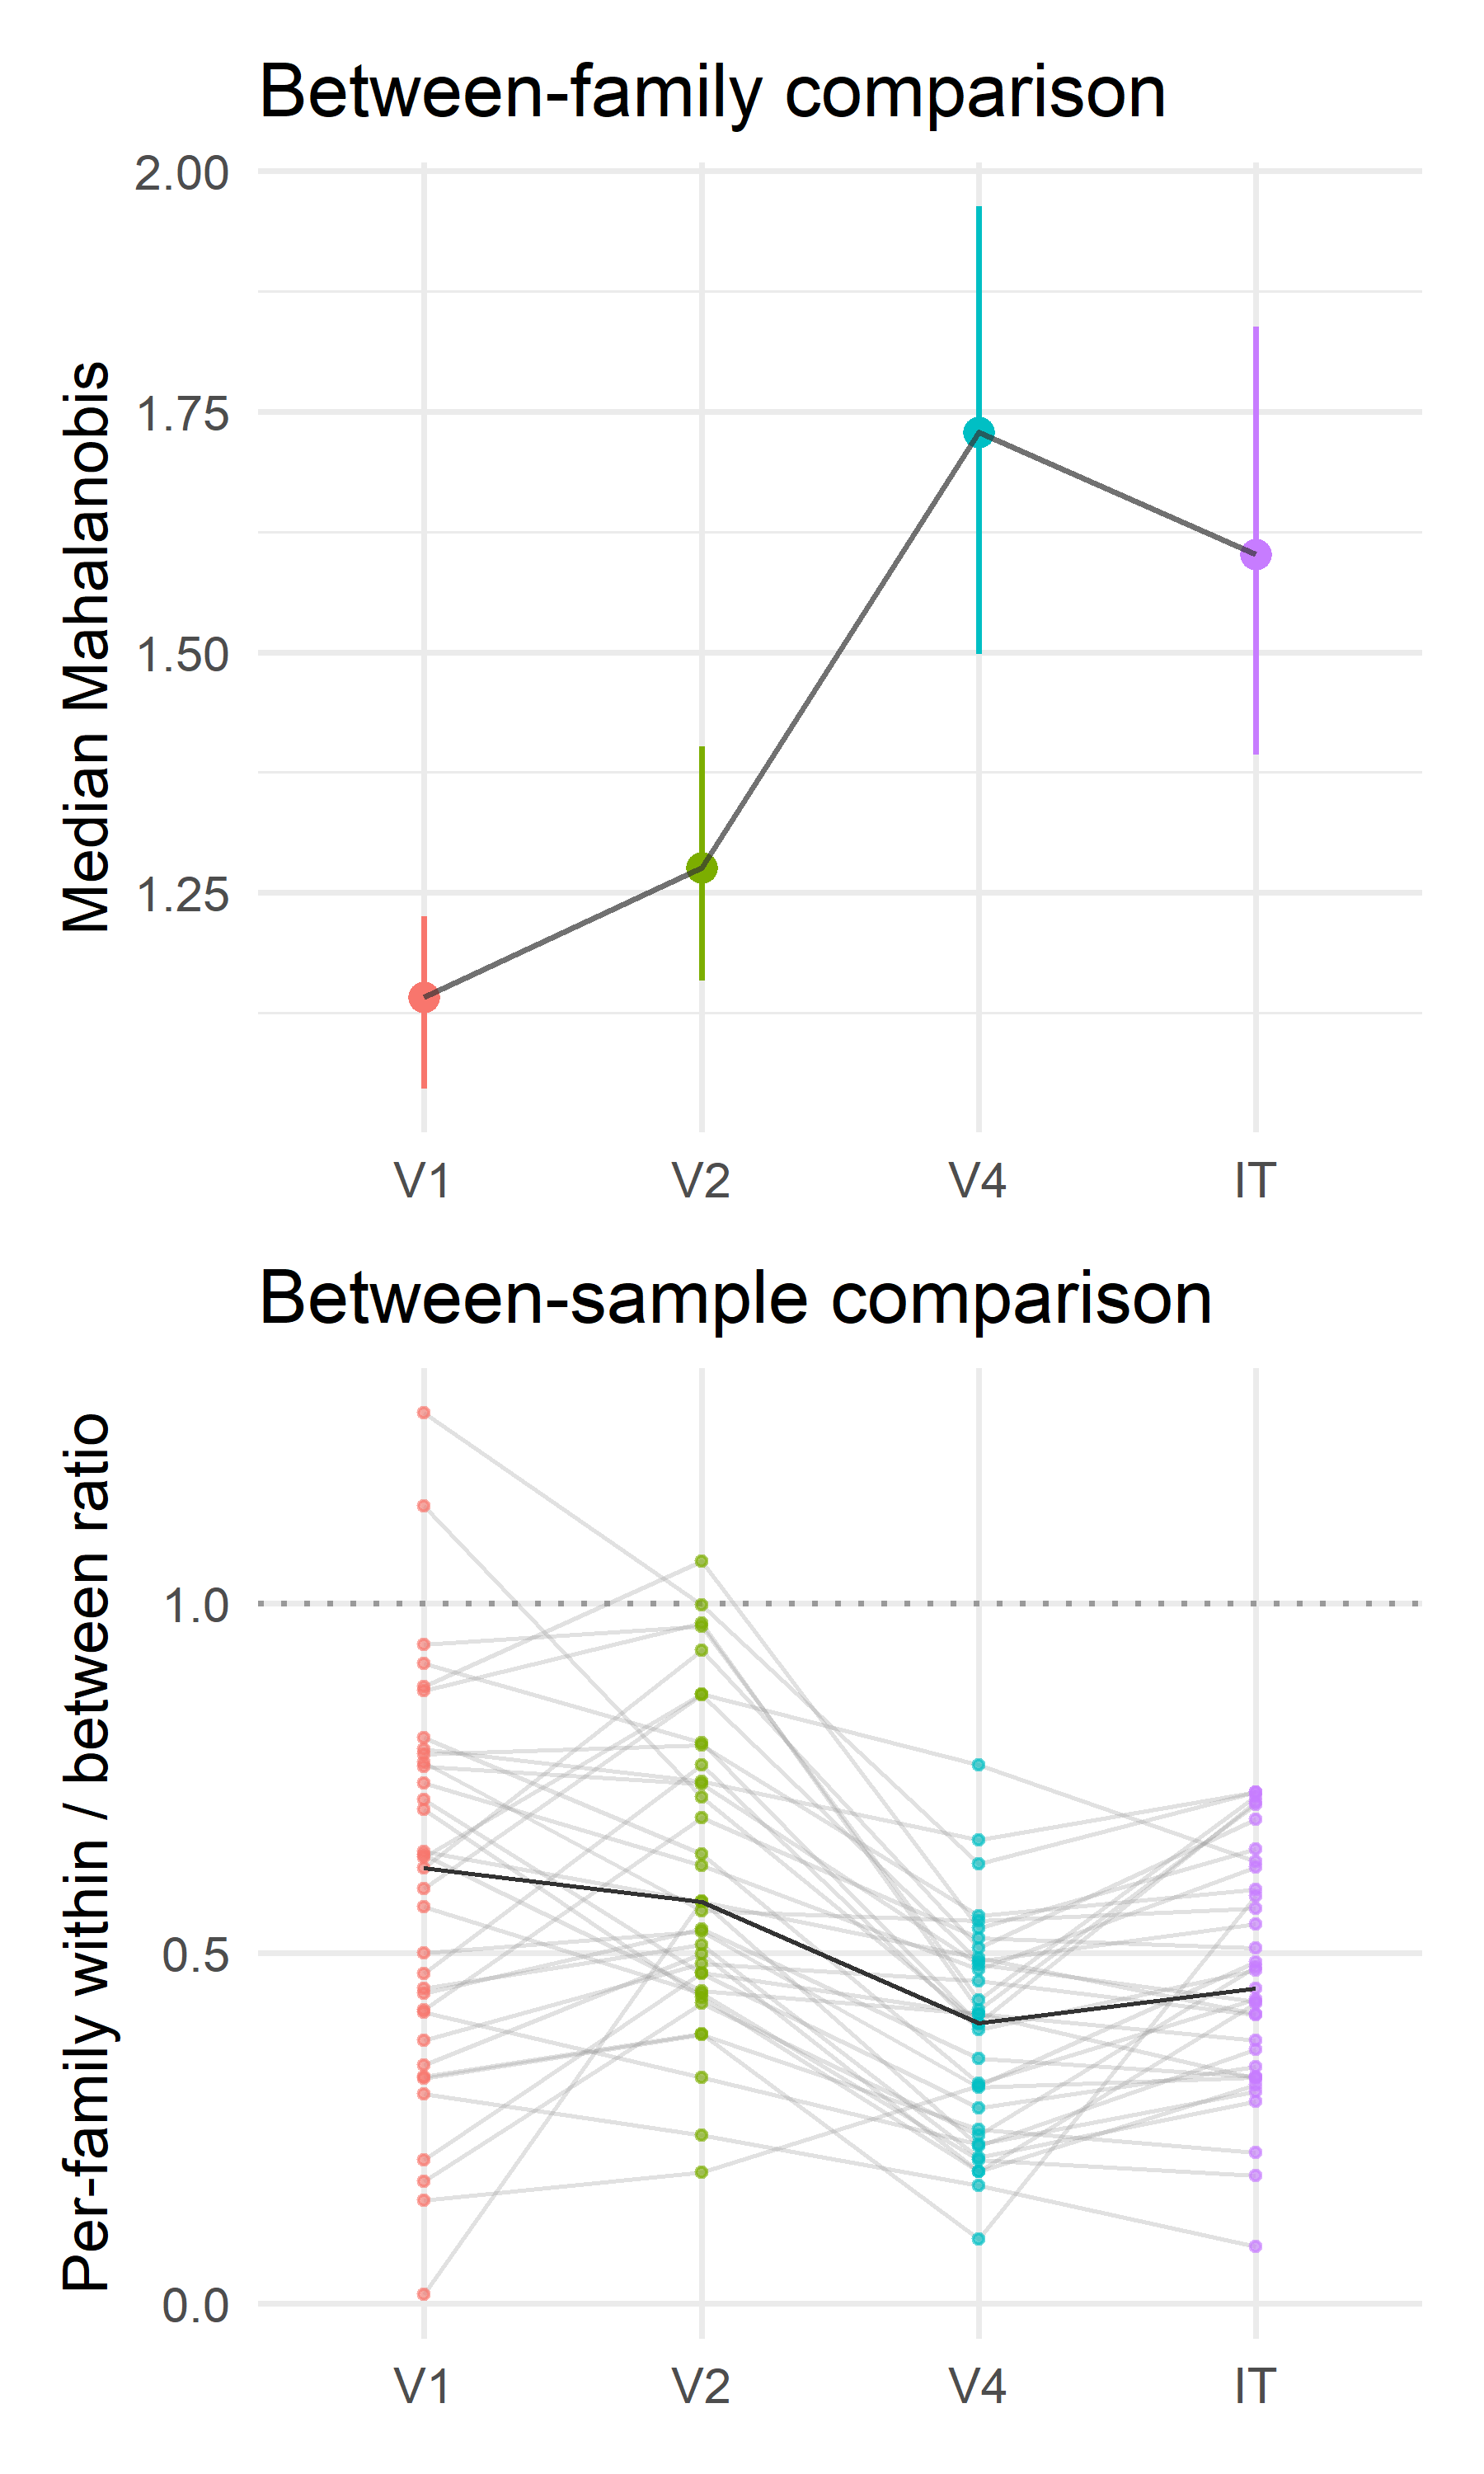
\includegraphics[width=\textwidth]{img/pf_ps_summary.png}
\end{column}
\end{columns}
\end{frame}

\begin{frame}{Overview}
\begin{columns}
\begin{column}{0.65\textwidth}
\begin{itemize}
    \item We characterize regions by the separability of visual textures \pause
    \item Differences in the \hl{reliability} and \hl{sparsity} bias these measures \pause 
    \item After correcting for reliability, IT texture separability appears comparable to V4 \pause
    \item V4 and IT show better between-family separation and worse within-family sample separation compared to V1 and V2
\end{itemize}
\end{column}
\begin{column}{0.35\textwidth}
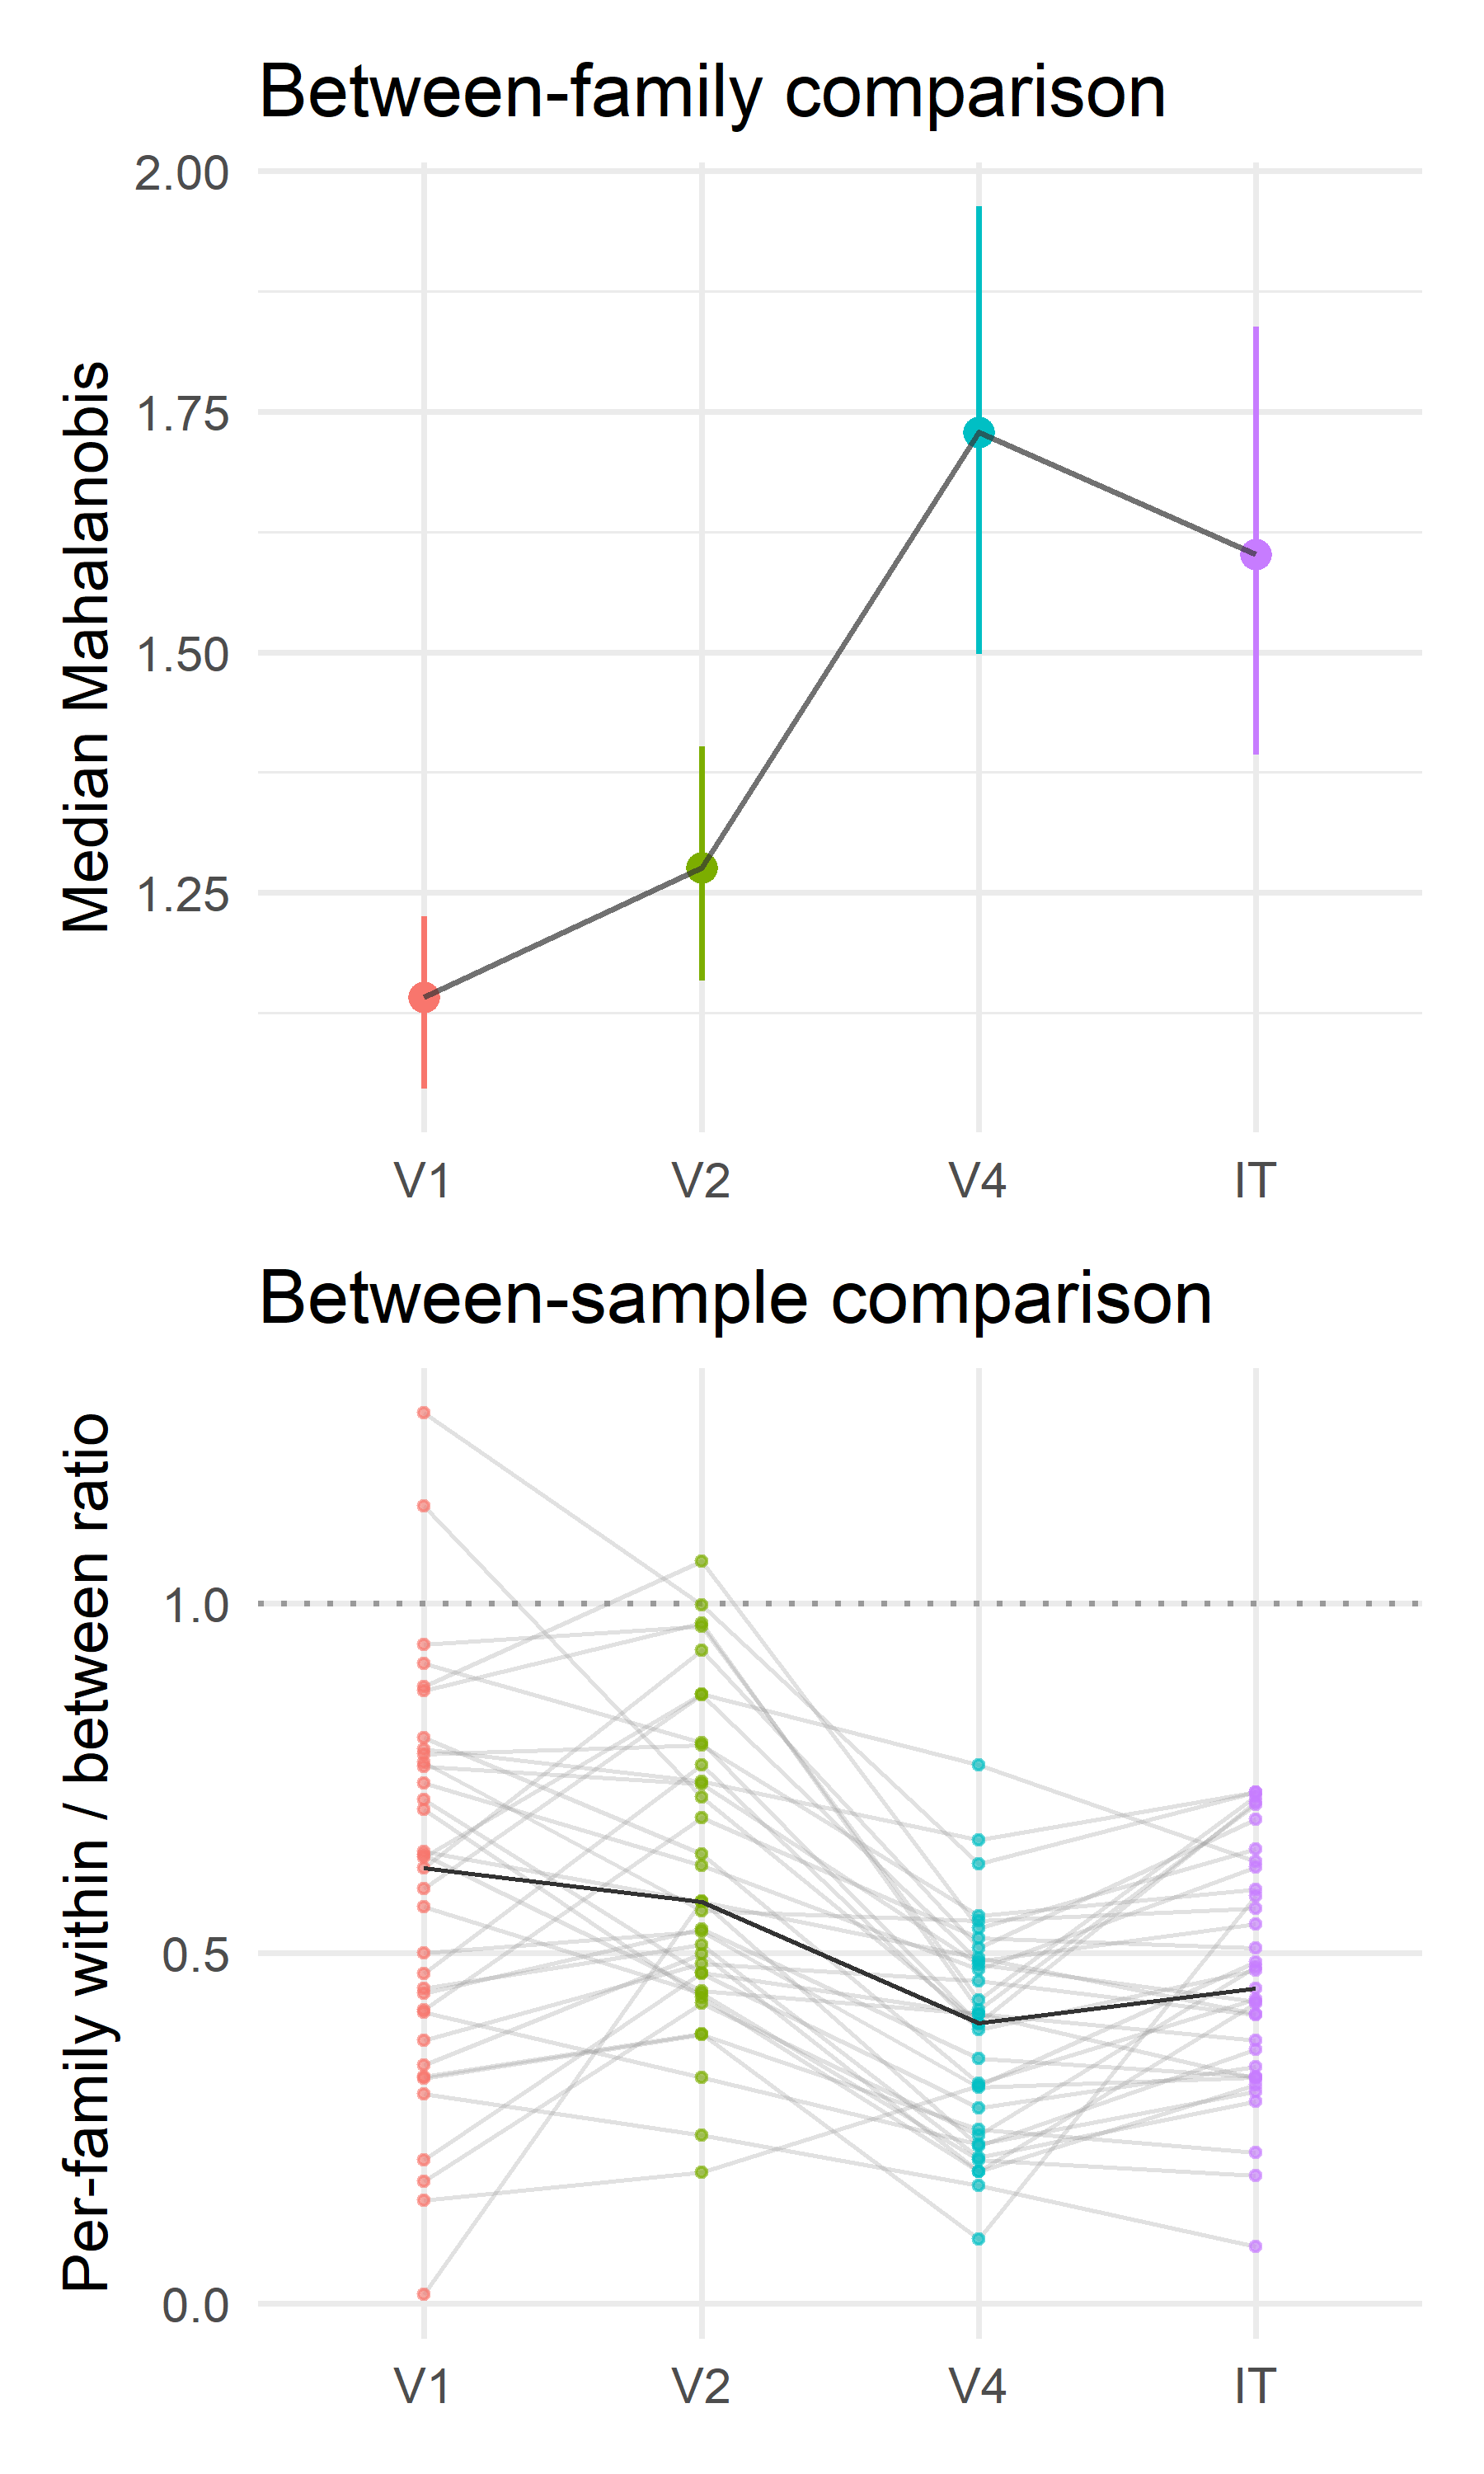
\includegraphics[width=\textwidth]{img/pf_ps_summary.png}
\end{column}
\end{columns}
\end{frame}



\section{Bibliography}
\begin{frame}[allowframebreaks]
\printbibliography
\end{frame}

\section{Additional slides }
\begin{frame}{Available sites for each region}
\centering
\begin{tabular}{crrrr|r}
Region & Array 1 & Array 2 & Array 3 & Array 4 & Total \\
\hline
V1 & 61 (M1) & 96 (M6) &         &         & 157 \\
V2 & 35 (M1) & 96 (M2) &         &         & 131 \\
V4 & 96 (M1) & 96 (M2) & 96 (M8) &         & 288 \\
IT & 96 (M3) & 96 (M6) & 96 (M6) & 96 (M7) & 384 \\
\end{tabular}

\begin{itemize}
    \item Monkey IDs in parentheses (\cite{lee_developmentally_2024})
    \item One array for M1 was implanted on the border of V1/V2, creating the 61/35 split in electrodes.
    \item Extra array in M6 implanted later in life after failure of earlier IT array
    \item ``Missing'' arrays not localized to a specific region; data discarded. 
\end{itemize}
\end{frame}


\begin{frame}{Reliability calculation}
\begin{enumerate}
    \item Split the six repetitions of each stimulus into two groups of three. 
    \item Average over the repetitions, producing two \( 35 \times 15 \)-length vectors. 
    \item Estimate Pearson's \( r \) and apply Fisher's \( z \)-transformation as \( \operatorname{artanh} (r) \) (\cite{kass_linear_2014})
    \item Repeat 1-3 for all \( \binom{6}{3} / 2 = 10 \) possible splits of the data. 
    \item Average the \( z \)-transformed results then invert Fisher's \( z \)-transformation, i.e., \( \hat{r} = \operatorname{tanh} \left( \frac{1}{10} \sum_{i = 1}^{10} \operatorname{artanh} (r_i) \right) \).
    \item To obtain the reliability estimate for six samples, apply the Brown-Spearman correction \( \rho = \frac{2 \hat{r}}{1 + \hat{r}} \).
\end{enumerate}

I examined how reliability shifts with onset times (earlier / median), window length (100 ms / 150 ms), blank image handling (none / aggregated / separated), and stimuli set (non-blank / noise / naturalistic).
\end{frame}

\begin{frame}{Reliability calculations in IT are more affected by onset shifts and window length}
\centering 
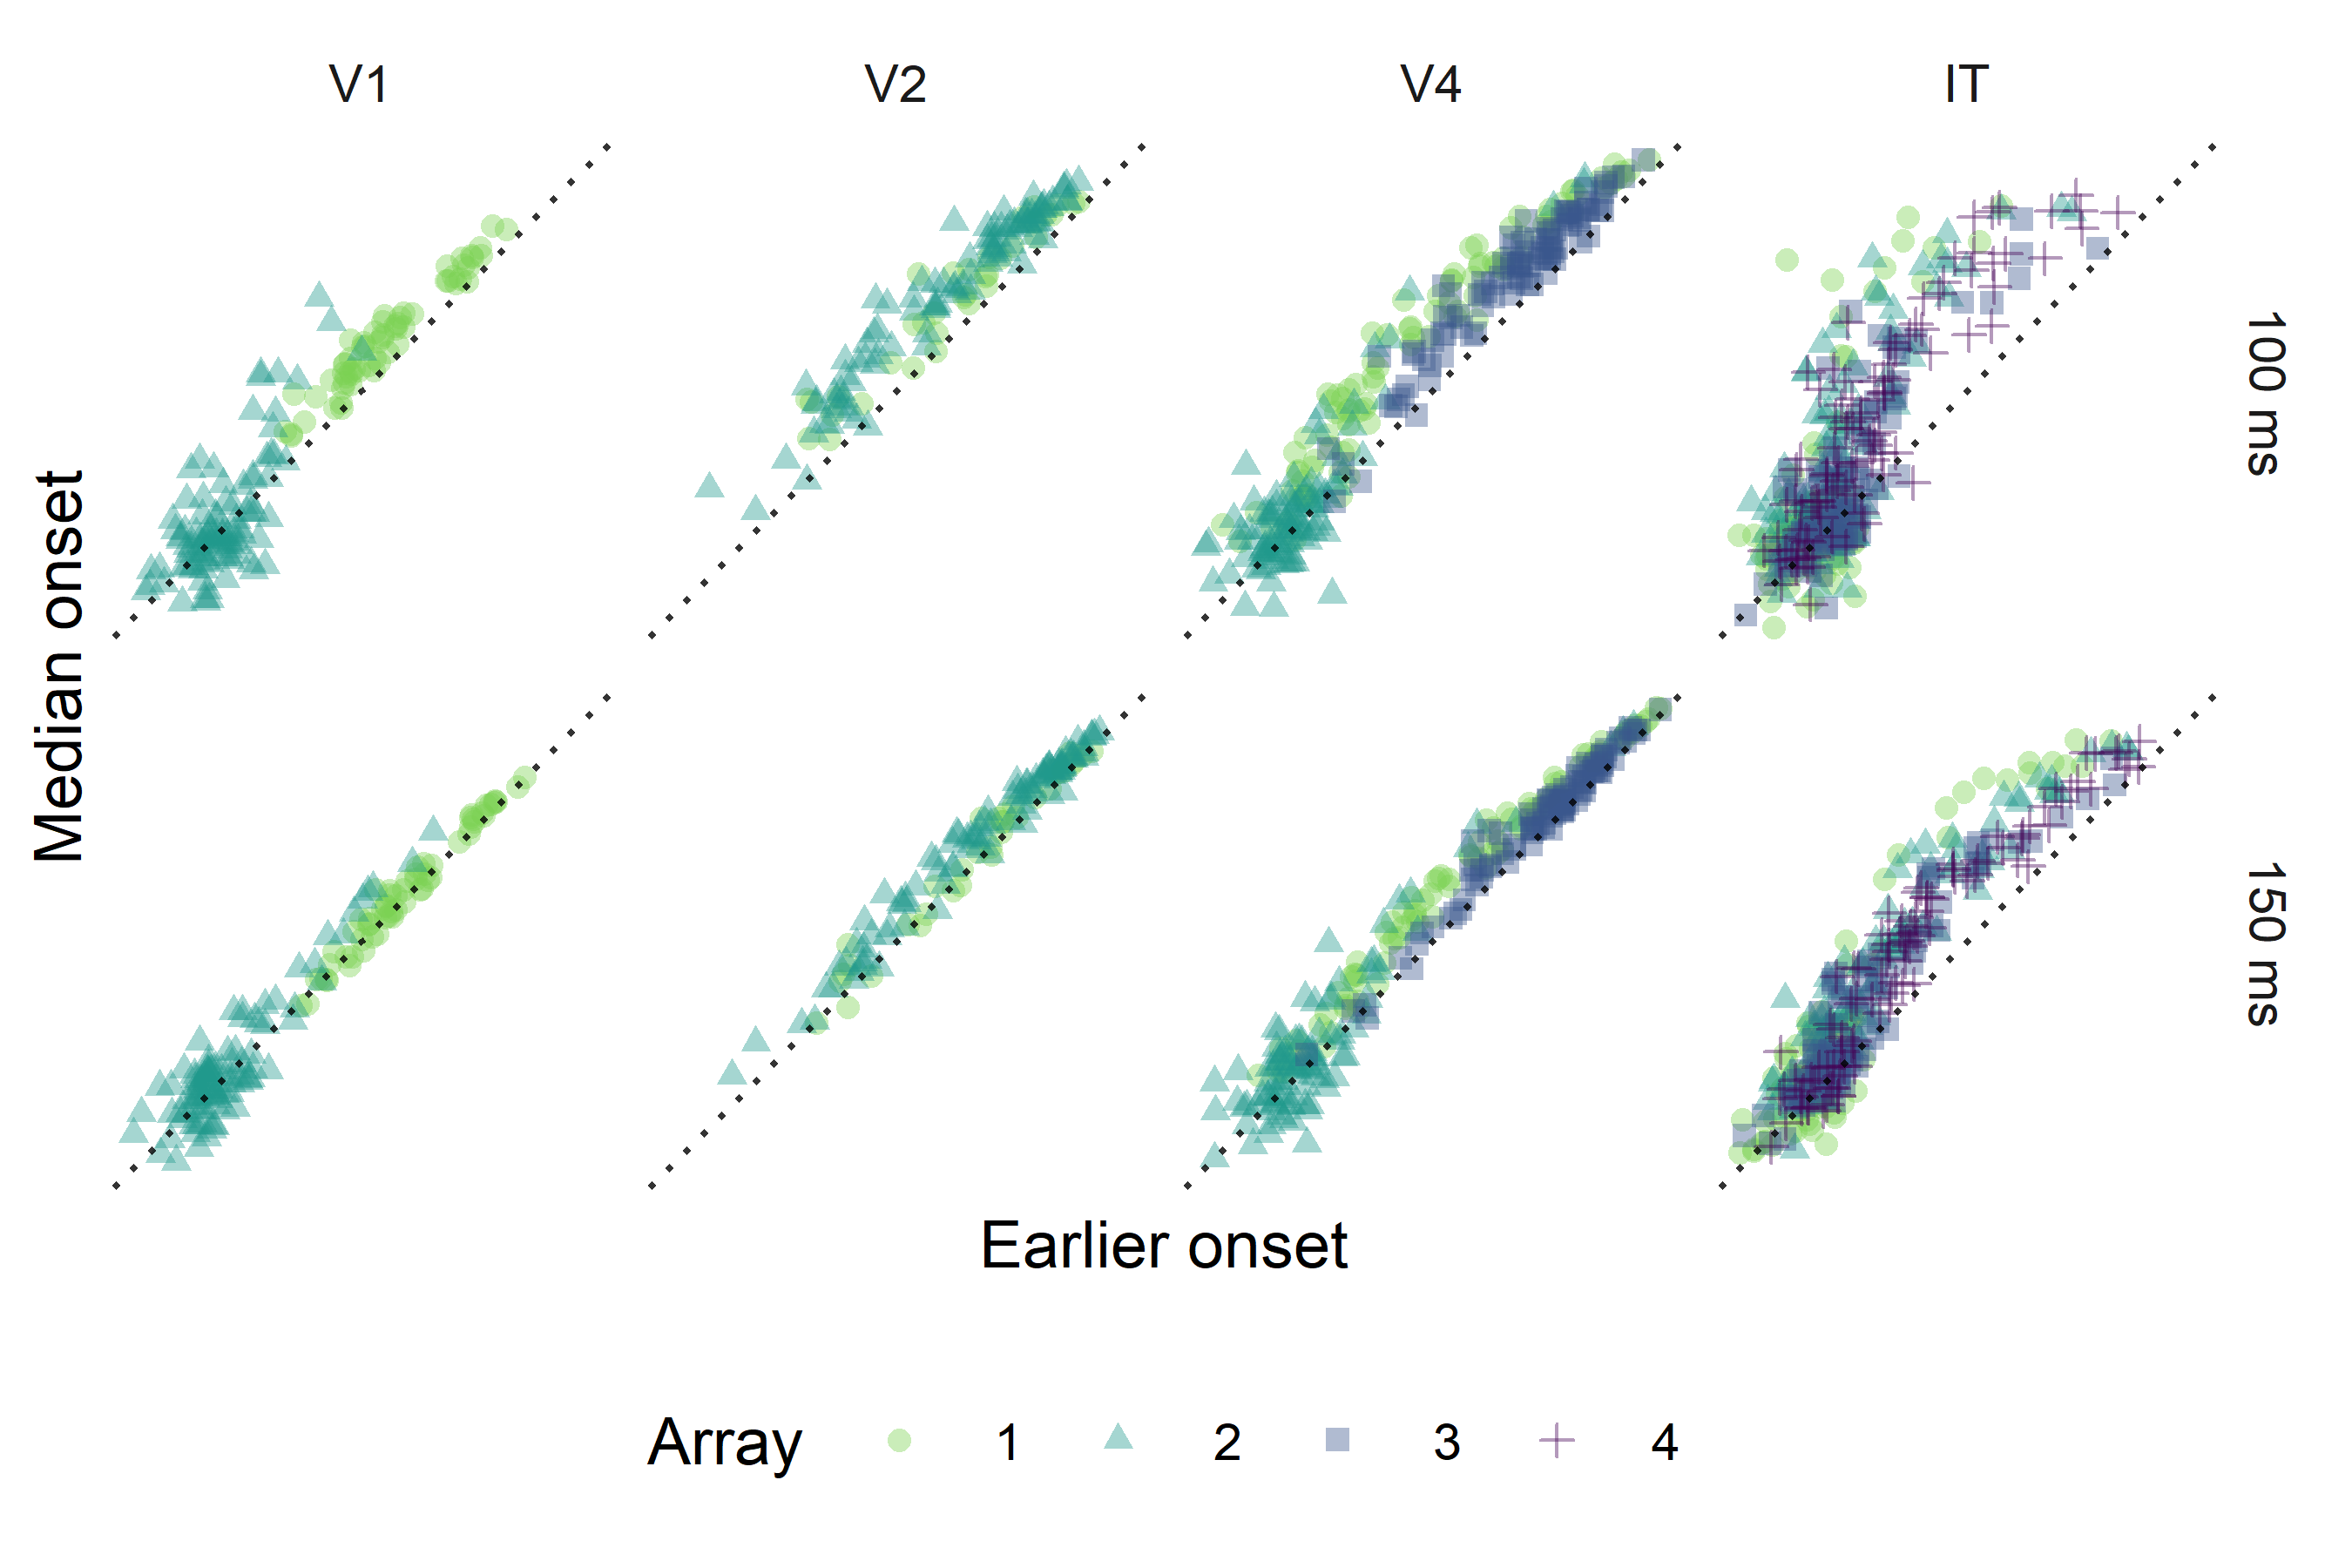
\includegraphics[width=0.7\textwidth]{img/early_median_windows.png}
\end{frame}

\begin{frame}{Proof of Mahalanobis robustness to normalization}
Let \( \mathbf{b} \in \mathbb{R}^k \) be some arbitrary constant vector and \( \mathbf{m} \in \mathbb{R}^k\) be some non-zero constant vector. If we take 
\begin{align*}
\bfx' &= \begin{bmatrix} m_1 x_1 + b_1 & m_2 x_2 + b_2 & \cdots & m_k x_k + b_k  \end{bmatrix}^\intercal, \\
\bfy' &= \begin{bmatrix} m_1 y_1 + b_1 & m_2 y_2 + b_2 & \cdots & m_k y_k + b_k  \end{bmatrix}^\intercal,
\end{align*}
then transform the assumed covariance matrix of the new distribution \( P \) accordingly with \[
\tilde{\boldsymbol{\Sigma}} = \diag (\mathbf{m}) \boldsymbol\Sigma \diag (\mathbf{m}), \] then the term in the Mahalanobis distance simplifies to
\begin{align*}
& (\bfx' - \bfy')^\intercal \tilde{\boldsymbol\Sigma}^{-1} (\bfx' - \bfy') \\
&= 
(\bfx - \bfy)^\intercal \diag (\mathbf{m}) \left(  \diag (\mathbf{m}) \boldsymbol\Sigma \diag (\mathbf{m}) \right)^{-1} \diag (\mathbf{m}) (\bfx - \bfy) \\
&= (\bfx - \bfy)^\intercal \boldsymbol\Sigma^{-1} (\bfx - \bfy).
\end{align*}
\end{frame}

\begin{frame}{(Cont.)}
Though the sample setting estimates the covariance rather than relying on the known \( P \), this invariance to centering and scaling still holds. That is, 
\begin{align*}
\hat{\boldsymbol\Sigma}_{\bfx'} &= \frac{1}{n_x - 1} \sum_{i = 1}^{n_x} (\bfx_i' - \overline{\bfx}') (\bfx_i' - \overline{\bfx}')^\intercal \\
&= \frac{1}{n_x - 1} \sum_{i = 1}^{n_x} \diag(\mathbf{m}) (\bfx_i - \overline{\bfx}) (\bfx_i - \overline{\bfx})^\intercal \diag (\mathbf{m}) \\
\bfx' - \bfy' &= \diag (\mathbf{m}) (\bfx - \bfy)
\end{align*}
and the calculated statistic remains the same. 
\end{frame}

\begin{frame}{Denoised (debiased) Treves-Rolls sparsity estimation}

Let \( m_i \) be the \( i \)th moment. Then, \( S_{\textrm{TR}} = (1 - a) (1 - 1 / N)^{-1}\), where \( a = m_1^2 / m_2 \). 

\textbf{Debiased denominator}: For a given stimulus \( i \), the plug-in estimator has expectation \( \E [ \bar y_i^2 ] = \mu_i^2 + \sigma_i^2 / K \), where \( \mu_i \) is the true mean response, \( \sigma_i \) is the variance in the response to stimulus \( i \), and \( K = 6 \) is the number of repetitions. 

Assuming independence of the repetitions to the same stimulus, the product of two different repetitions is unbiased, i.e., \( \E[y_{i, k} y_{i, l}] = \mu_i^2 \). Define \( \widehat{\mu_i^2} \) as the mean of these products over all \( \binom{6}{2} \) pairs of repetitions. Then, \( \hat m_2 \) is the mean of these \( \widehat{\mu_i^2} \). 

\textbf{Debiased numerator}: Within \( \left( \sum_i \bar y_i \right)^2, \) the same-stimulus terms can be replaced with \( \widehat{\mu_i^2} \). The cross-stimulus products are already unbiased.

\textbf{Limiations}: The debiased estimator may be negative. At very low reliability, the procedure might be unstable (hence the reliability filter in the slide). 
\end{frame}

\end{document}

\begin{frame}{Additional slides}
\end{frame}

\begin{frame}{Pointwise and joint confidence interval construction}

\end{frame}

\begin{frame}{Simulation results}
\end{frame}

\begin{frame}{Extension to generalized linear mixed models}
\begin{itemize}
    \item There is no analytic form for the pointwise and joint CIs. 
\end{itemize}
\end{frame}